\documentclass[a4paper, 12pt]{report}
\usepackage[utf8]{inputenc}
\usepackage[toc,page]{appendix}
\usepackage{graphicx}
\graphicspath{ {images/} }
\usepackage[english]{babel}
\usepackage{listings}
\usepackage{scrextend}
\usepackage{xcolor}
\usepackage{csquotes}
\usepackage{setspace}
\usepackage{stmaryrd}
\usepackage{multirow}
\usepackage{amsthm}
\usepackage{tikz}
\usetikzlibrary{positioning}
\usepackage{amsfonts}
\newtheorem{definition}{Definition}
\usepackage{caption}
\usepackage{amssymb}% http://ctan.org/pkg/amssymb
\usepackage{pifont}% http://ctan.org/pkg/pifont
\newcommand{\cmark}{\ding{51}}%
\newcommand{\omark}{\ding{109}}%
%\DeclareCaptionFormat{myformat}{#1#2#3\hrulefill}
%\captionsetup{format=myformat}
%\captionsetup[lstlisting]{position=bottom,format=myformat}
% LANGUAGE SETUP FOR LISTINGS

\theoremstyle{definition}

\newtheorem{exmp}{Example}


\usepackage{color}
\definecolor{purple}{rgb}{0.65, 0.12, 0.82}
\definecolor{darkgreen}{rgb}{0.13, 0.54, 0.13}

\lstdefinelanguage{JavaScript}{
  keywords={typeof, new, true, false, catch, function, return, null, catch, switch, var, if, in, while, do, else, case, break},
  keywordstyle=\color{blue}\bfseries,
  ndkeywords={class, export, boolean, throw, implements, import, this},
  ndkeywordstyle=\color{blue}\bfseries,
  identifierstyle=\color{black},
  sensitive=false,
  comment=[l]{//},
  morecomment=[s]{/*}{*/},
  commentstyle=\color{darkgreen}\ttfamily,
  stringstyle=\color{red}\ttfamily,
  morestring=[b]',
  morestring=[b]"
}

\lstdefinelanguage{JSON}{
  keywords={test},
  keywordstyle=\color{blue}\bfseries,
  ndkeywords={testo},
  ndkeywordstyle=\color{blue}\bfseries,
  identifierstyle=\color{black},
  sensitive=false,
  comment=[l]{//},
  morecomment=[s]{/*}{*/},
  commentstyle=\color{darkgreen}\ttfamily,
  stringstyle=\color{black}\ttfamily,
  morestring=[b]',
  morestring=[b]"
}

\lstset{
   language=JSON,
   extendedchars=true,
   basicstyle=\footnotesize\ttfamily,
   showstringspaces=false,
   showspaces=false,
   numbers=left,
   numberstyle=\footnotesize,
   numbersep=9pt,
   tabsize=2,
   breaklines=true,
   showtabs=false,
   captionpos=b,
   frame=tb
}

\lstdefinelanguage{JSQL}{
  keywords={G, state, wildcard, skipZeroOrMore, lBrace, rBrace, star, plus, not},
  keywordstyle=\color{blue}\bfseries,
  ndkeywords={this, properties, lookup, value, filters, node, benv, store},
  ndkeywordstyle=\color{purple}\bfseries,
  identifierstyle=\color{black},
  sensitive=false,
  comment=[l]{//},
  morecomment=[s]{/*}{*/},
  commentstyle=\color{darkgreen}\ttfamily,
  stringstyle=\color{red}\ttfamily,
  morestring=[b]',
  morestring=[b]"
}

\lstset{
   language=JSQL,
   extendedchars=true,
   basicstyle=\footnotesize\ttfamily,
   showstringspaces=false,
   showspaces=false,
   numbers=left,
   numberstyle=\footnotesize,
   numbersep=9pt,
   tabsize=2,
   breaklines=true,
   showtabs=false,
   captionpos=b,
   frame=tb
}

\lstset{
   language=JavaScript,
   extendedchars=true,
   basicstyle=\footnotesize\ttfamily,
   showstringspaces=false,
   showspaces=false,
   numbers=left,
   numberstyle=\footnotesize,
   numbersep=9pt,
   tabsize=2,
   breaklines=true,
   showtabs=false,
   captionpos=b,
   frame=tb
}

\usepackage{blindtext}
\usepackage{enumitem}
%\usepackage[style=apa,backend=biber,language=american]{biblatex}
%\DeclareLanguageMapping{american}{american-apa}
\usepackage[backend=biber,style=numeric,citestyle=numeric]{biblatex}
\addbibresource{references.bib}
% The following makes latex use nicer postscript fonts.
\usepackage{times}
 
% get clickable links
% http://stackoverflow.com/questions/3244803/latex-add-clickable-links-to-a-section-subsection-with-a-pdf-document
\usepackage{hyperref}
\hypersetup{
  colorlinks   = true,    % Colours links instead of ugly boxes
  urlcolor     = blue,    % Colour for external hyperlinks
  linkcolor    = black,    % Colour of internal links
  citecolor    = black      % Colour of citations
}
 
 
%\usepackage[backend=biber,style=numeric,citestyle=authoryear]{biblatex}
%\usepackage{biblatex}
\makeatletter
% http://tex.stackexchange.com/questions/61204/autocomplete-in-texniccenter-does-not-work-when-biblatex-is-used
% "Since TeXnicCenter does not check for if clauses, it just assumes \bibliography has been used and binds it into the GUI."
%\@ifpackageloaded{biblatex}{\addbibresource{references.bib}}{\bibliography{references}}
\makeatother
       
\usepackage{vubtitlepage}
 
\usepackage{listings}
\hyphenation{mul-ti-di-rec-tio-na-li-ty}
 
\author{Valentijn Spruyt}
\title{Static detection of user-specified \\ security vulnerabilities in client-side\\ JavaScript}
\promotor{Prof. Dr. Coen De Roover}
\advisors{Jens Nicolay\\
         Quentin Sti\'{e}venart}
\degree{Master of Science in de Ingenieurswetenschappen: Computerwetenschappen}
\faculty{Faculty of Science and Bio-Engineering Sciences}
\advisortitle{Advisors}
\department{Department of Computer Science\\ and Applied Computer Science}
\reason{Graduation thesis submitted in partial fulfillment of the
requirements for the degree of} 

\date{JUNE 2016}
 
\begin{document}

\maketitlepage
 
\advisortitle{Begeleiders}
\faculty{Faculteit Wetenschappen en Bio-\\Ingenieurswetenschappen}
\department{Departement Computerwetenschappen\\en Toegepaste Informatica}
 
\reason{Proefschrift ingediend met het oog op het behalen van de graad
van} %\\
%Master of Science in de Ingenieurswetenschappen: Computerwetenschappen}
\date{JUNI 2016}
 
\maketitlepage


\pagenumbering{roman} % Start roman numbering
\chapter*{Abstract}

%Why
Program defects tend to surface late in the development of programs, and they are hard to detect.
%TODO: security vulnerabilities, such as ..
The same goes for security vulnerabilities. This type of program defects is particularly important to detect as they might leak sensitive information or even compromise the system on which the program is executed.
%TODO: Tools static, + benefit: goed omdat at compile time

A popular approach for analyzing programs is static analysis. Static analysis of a program is performed at compile time, implying that the program can be analyzed without being executed.
 Existing approaches using static analysis to detect security vulnerabilities in source code are often limited to a predetermined set of pre-encoded security vulnerabilities. Although these approaches are able to detect a decent amount of vulnerabilities and support a wide range of programs by default, they lack the means to be configured for vulnerabilities that are specific for the particular application domain of the analyzed program.

%What in thesis onderzocht
In this dissertation, we investigate how static analysis can aid in detecting application-specific security vulnerabilities. As these vulnerabilities are not general enough to be checked by tools that use a database of pre-encoded patterns, developers should be able to write rules that are specifically applicable to their program. 

%Hoe
We present JS-QL, a tool for statically checking user-specified security vulnerabilities in JavaScript applications. The tool makes use of an embedded domain-specific query language built on top of JavaScript. JS-QL queries are based on regular path expressions, enabling users to express queries in an intuitive way. These expressions are a way of declaratively expressing queries on graphs as regular-expression-like patterns. In the context of this dissertation, regular path expressions are used to match user-specified patterns on an abstract state graph, which is generated as the output of performing static analysis. 

%Resultaten
We evaluated our approach by comparing our language with other languages for expressing security vulnerabilities in terms of expressiveness. We conclude that the combination of static analysis and regular path expressions lends itself well to the detection of user-specified security vulnerabilities.

\chapter*{Samenvatting}

Tekortkomingen in programma's zijn moeilijk te detecteren en ze komen vaak pas laat aan de oppervlakte in het ontwikkelingsproces. Hetzelfde geldt voor beveiligingslekken. Dit soort van kwetsbaarheden is uitermate belangrijk om op te sporen, aangezien ze mogelijks geheime informatie lekken of er zelfs voor kunnen zorgen dat het systeem waarop het programma draait gecomprommiteerd wordt.
 
Een populaire aanpak om programma's te analyseren is statische analyse. Statische analyse van een programma wordt uitgevoerd at compile time, wat betekent dat het programma kan geanalyseerd worden zonder het uit te voeren. Bestaande oplossingen die gebruik maken van statische analyse om beveiligingslekken op te sporen in broncode zijn vaak beperkt tot een voorafbepaalde set van voorgeprogrammeerde programmapatronen. Hoewel deze oplossingen een redelijk aantal kwetsbaarheden in programma's vinden, ontbreken ze een manier om geconfigureerd te worden om kwetsbaarheden te vinden binnen het domein van het geanalyseerde programma.

In dit proefschrift onderzoeken we hoe statisch analyse kan helpen om programmaspecifieke beveiligingslekken te detecteren. Aangezien deze beveiligingslekken niet algemeen genoeg zijn om gevonden te worden door tools die een databank van voorgeprogrammeerde patronen gebruiken, zouden ontwikkelaars de mogelijkheid moeten hebben om zelf patronen te schrijven die toepasbaar zijn op hun specifieke programma's.

We stellen JS-QL voor, een tool om op statische manier beveiligingslekken, gespecificeerd door de gebruiker, in JavaScript applicaties te detecteren. De tool gebruikt een embedded domein-specifieke querytaal die gebouwd is bovenop JavaScript. JS-QL queries zijn gebaseerd op regular path expressions die de gebruiker er toe in staat stellen queries uit te drukken op een intuitieve manier. Regular path expressions zijn een manier om declaratief queries op graphs uit te drukken, gelijkaardig aan de notatie van reguliere expressies. Binnen de context van dit proefschrift worden regular path expressions gebruikt om patronen, gespecificeerd door gebruikers, te matchen tegen een abstract state graph die gegenereerd wordt als output van statische analyse.

We hebben onze aanpak geëvalueerd door onze taal op vlak van expressiviteit te vergelijken met andere talen waarin beveiligingslekken uitgedrukt kunnen worden. We besluiten dat de combinatie van statische analyse en regular path expressions zich goed leent tot het opsporen van beveiligingslekken die door de gebruiker gespecificeerd zijn.

\chapter*{Acknowledgements}
 
%ouders for opportunity
I am most thankful towards my promotor Coen De Roover and my supervisors Jens Nicolay and Quentin Sti\'{e}venart for their valuable advice and helpful comments throughout the year. They helped me focus on the important parts of my thesis and kept me motivated. I would also like to thank my friends Jonas and Dylan for their support and encouragement to keep working on this dissertation, even in periods when I lacked motivation. I admire my loving girlfriend for standing by my side through this period and for putting up with my stressful behaviour. I am also grateful for the opportunity my parents gave me to go to university to get my masters degree. Finally, I would also like to thank my friend Ben for reading most parts of this work. I appreciate his comments and insights greatly.

\tableofcontents

\listoffigures
\listoftables


\chapter{Introduction}
\setcounter{page}{1}
\pagenumbering{arabic} % Start roman numbering 


%korte intro waarover thesis gaat
This dissertation investigates how static analysis can help developers to statically verify user-defined and application-specific security policies. Checking a program for security vulnerabilities using static analysis has as a benefit that the program does not have to be executed.
% Static analysis benefits from the fact that a program does not have to be compiled to check for program properties, defects and security vulnerabilities. 
Our thesis is that \textit{a specification language based on regular path expressions can be used to effectively express patterns for detecting security vulnerabilities. These vulnerabilities are then searched for in source code by checking them against the output of the performed static analysis.}

Program defects tend to surface late in the development of programs, and they are hard to detect. The same goes for security vulnerabilities. This type of program defects is particularly important to detect as they might leak sensitive information or even compromise the system on which the program is executed. Existing approaches using static analysis to detect security vulnerabilities in source code are often limited to a predetermined set of pre-encoded security vulnerabilities. Although detecting a decent amount of vulnerabilities and supporting a wide range of programs by default, they lack the means to be configured for vulnerabilities that are specific for the particular application domain of the analyzed program. It therefore is important to be able to write succinct queries to test a program against \textit{application-specific} flaws, as most programs differ in behaviour which makes it difficult to write a simple query or pre-encoded rule for a set of different programs. 

We present JS-QL, an embedded domain-specific specification language based on regular path queries, built on top of JavaScript. This language enables expressing queries in the native JavaScript language in such a way that queries remain readable and that expressiveness is maximized. In our approach to detect security vulnerabilities, JS-QL is used in combination with static analysis to check \textit{user-defined} queries against an abstract state graph, which is a the representation of a program's runtime behaviour resulting from the analysis.


\section{Objectives and contributions}
The use of Javascript for native and web applications is increasing. This has as consequence that malicious users get more creative and passionate about finding security vulnerabilities in these applications and that more of these vulnerabilities are exploited. Developers of applications should be armed with appropriate tools to find these vulnerabilities before their application gets deployed. We present such a tool that can be configured to detect vulnerabilities using a domain-specific specification language. Our contributions are the following:
\begin{enumerate}
\item We investigate which type of specification language is best suited to express security vulnerabilities and program characteristics in general. We believe that regular path expressions are a suitable means as they are expressive and easy to reason about. We evaluate our specification language by expressing multiple security vulnerabilities and comparing the resulting specifications to corresponding ones of existing work.
\item We present the JS-QL \textit{domain-specific language}, a language built to express succinct and highly readable program queries. The application-specific nature of the queries written in the language together with the possibility for users to define these queries by themselves makes it a powerful aid in checking program characteristics and, more precisely, security vulnerabilities. In contrast to general program checkers, a much wider range of program characteristics can be detected.
\item Specifying security vulnerabilities is one thing, checking them against a program is another. To this extent, we have developed a \textit{tool} to match the queries specified in JS-QL against JavaScript programs. The tool supports multiple types of queries, allowing developers to explore their program in several ways. A simple user interface handles all communication with the user, meaning that both input information (the query and the input program) and the output results (all found matches) are displayed in a single window. Although queries are evaluated through the user interface, compound queries can be written and saved in a separate file and are instantly available to the user.
\end{enumerate} 

\section{Overview}

Chapter \ref{ch:Background} discusses the detection of security vulnerabilities. We first give an introduction to static analysis (Section \ref{sec:staticAnalysis}). We discuss the basics of static analysis as well as a static analysis technique called abstract interpretation. Next, we review existing work for detecting generic vulnerabilities in programs (Section \ref{sec:genericVulnerabilities}). As the goal of this dissertation is to explore a way to express application-specific queries for detecting program vulnerabilities, we also describe some application-specific approaches to query for program characteristics and security vulnerabilities (Section \ref{sec:applicationSpecificVulnerabilities}). In this chapter we show that the approach that seems most apt for this thesis is to combine regular path queries with an abstract state graph.

In chapter \ref{ch:Overview} an overview of our approach is given. We sketch the architecture of our tool and briefly discuss what the roles of each component are (Section \ref{sec:Architecture}). As we traverse an abstract state graph to obtain program information, the user has to have knowledge of what information is contained in this graph. We go into greater detail about the information contained in each type of graph node in section \ref{sec:FlowGraphs}. The language developed in this dissertation is a so-called internal domain-specific language (DSL) built on top of JavaScript. Section  \ref{sec:DSLForQueryingGraphs} discusses the benefits of domain-specific languages over general-purpose languages and compares internal domain-specific languages with external ones. Finally, this chapter also explains some of the design constraints for building a domain-specific language as well as design patterns used to implement the JS-QL language (Section \ref{sec:DesignInternalDSL}).

The syntax, semantics and usage of the JS-QL language is explained in chapter \ref{ch:JSQL}. We describe all syntactic aspects of the language in section \ref{sec:Syntax}. Our implementation supports multiple types of queries, such as \textit{existential} and \textit{universal} queries, imposing different rules for a query to produce results. We also explain the difference between \textit{forward} and \textit{backward} queries, in section \ref{sec:TypesOfQueries}. The most important contribution of our approach is its support for user-defined and application-specific queries. In section \ref{sec:DefiningPolicies} we describe how queries in JS-QL should be written by means of examples.

Chapter \ref{ch:Implementation} describes how the tool is implemented and how components work together. We explain how the user interface is implemented and how it sends data to the DSL-layer. We further discuss how this data is processed as well as how the DSL is built. As the matching of the abstract state graph and the query pattern is the core of our tool, we invest in explaining how the matching engine works.

We report on the results of evaluating our approach in chapter \ref{ch:Evaluation} by expressing security vulnerabilities originating in related work. We checked if and how we can express these queries in JS-QL and evaluated the query verboseness, flexibility, expressiveness and readability. In this chapter we show that JS-QL is well-suited to specify different kinds of security vulnerabilities, but some specifications concerning dependencies in a program remain hard to express. 

We conclude in chapter \ref{ch:Conclusion}, and give an overview of the limitations of our approach and provide some topics for future research.


\chapter{Detecting security vulnerabilities}
\label{ch:Background}
\begin{definition}
\textit{A \textbf{security vulnerability} is a weakness in a product that could allow an attacker to compromise the system's integrity, availability and confidentiality.} 
\end{definition}

To check for these vulnerabilities we need a program representation containing specific information about the program to be able to answer questions about security vulnerabilities. The information we need in this dissertation is twofold:

\begin{enumerate}
\item \textit{Control flow}: A program can contain many branches, loops and other control structures. We need to know the exact order of execution along each path in the program before we can make assumptions about security vulnerabilities. Therefore information is needed about which functions can be applied at a call site.
\item \textit{Value flow}: Variables in JavaScript are mutable, so their values can change at any moment in a program. Value flow information tells us exactly what values an expression may evaluate to. This is very important w.r.t. security, as a variable bound to a harmless value may get assigned a harmful value somewhere in the program. From there on, that variable should be marked as a possible threat to the system.
\end{enumerate}

A technique is needed to efficiently express security checks in the form of user-specified, application specific security policies. A naive way to examine programs would be to run them and keep track of any relevant information during execution. Not only would this be tiresome, we can also not guarantee that the program will ever terminate, that it terminates without errors, or that it will have the same outcome for different inputs. A better approach would be to to analyze the program \textit{without} having to run it. A field of research called \textit{static analysis} accommodates for this.

This chapter describes how static analysis can be used to examine programs and how this analysis can be addressed to obtain information about specific parts of a program. First, section \ref{sec:staticAnalysis} describes more precisely what static analysis is and why this technique is interesting in the context of this dissertation. Next, We discuss four approaches using static analysis to find generic vulnerabilities in programs in section \ref{sec:genericVulnerabilities}. Finally, four application-specific approaches for checking security vulnerabilities are discussed. For these approaches we take a deeper look on how they query the information. We end this chapter by giving a brief conclusion.

\section{Introduction to static analysis}
\label{sec:staticAnalysis}

\begin{definition}
\textit{\textbf{Static analysis} is a technique for analyzing computer programs without having to execute them and still obtain useful results.}
\end{definition}

Rice's theorem states that the ability to decide non-trivial program properties is equivalent to the ability to decide whether a program halts (halting problem), which implies that deciding non-trivial program properties is undecidable. As proving non-trivial program properties is undecidable, static analysis focuses on the instances of the problem about which it can tell whether the program satisfies a property or not, and leaves other instances unsolved. In this way we can avoid the possible problems we might encounter using a naive technique (e.g. manually tracking information flow during execution). The results of the analysis may indicate program defects or can be used to prove certain properties of the program.  The results of the static analysis will then be a useful set of approximate solutions. Figure \ref{fig:decider} shows the main difference between a regular decider, which will always provide an exact answser, and a static analyzer.

\begin{figure}[!h]
    \centering
      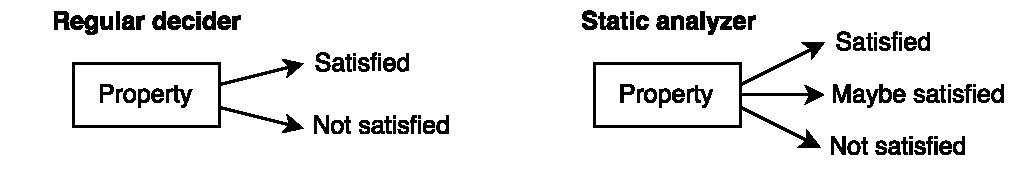
\includegraphics[width=0.9\textwidth]{images/decider} 
      \caption{Proving program properties: Regular decider and static analyzer}
    \label{fig:decider}
\end{figure}

\subsubsection*{Precision}

\textit{Precision} is very important in static analysis. Consider a static analyzer that concludes for each property that it is \textit{maybe} satisfied. It is clear to see that there is no precision in this analysis, rendering it useless. We have to strive to attain enough precision to solve the maximum number of problem instances. For our approach, precision is of great importance as we need to minimize the amount of false positive and true negatives.


\subsubsection*{Speed}

In the context of this dissertation, \textit{speed} is less important for the analysis. As static analysis is decidable, it is guaranteed that the analysis will run in finite time, but gathering precise results is much more meaningful than the performance of the analysis itself.
\\\\
\noindent A technique used for static analysis is \textit{abstract interpretation}. This technique mimics interpretation of a program and allows to stay close to the original language semantics of a program without having to modify or instrument it to perform the analysis (in contrast to other static analysis techniques such as \textit{symbolic execution}). This technique fits well for this dissertation, as we need to check for application-specific security vulnerabilities. It is thus a prerequisite that the semantics of the analyzed program lean as close to the original semantics as possible.
% A feature of abstract interpretation is that it allows to specify the precision needed by parameterizing it with e.g. a \textit{lattice}.

\subsection{Abstract interpretation}
%Quentin thesis
Abstract interpretation is a static analysis technique used to reason about a program. It does this by interpreting an approximation of a program through abstraction of its semantics. A \textit{sound} analysis can be performed and the precision of this analysis can be adjusted to the user's needs through various mechanisms. This increase in precision comes at the cost of a greater analysis running time. 

\subsubsection*{Concrete interpretation}

Abstract interpretation works in a similar way as normal program interpretation (i.e. \textit{concrete interpretation}). The concrete interpretation of a program can be described as follows: A program \textit{e} can be injected into an initial state \textit{$s_0$}, the entry point of the program. From this state other reachable states can be computed using a \textit{transition function}, until after several transitions a final state is reached. If no such state is ever reached, the execution will not terminate and hence will run indefinitely. The output of interpreting a program like this is a possibly infinite trace of execution states. The layout of this execution trace might depend on the input of the program or other changing values, making it unsuitable for static analysis. 

\subsubsection*{Applying abstraction}
Abstract interpretation solves the problem of the uncertainty introduced by concrete interpretation by applying abstraction in order to compute a finite trace. Sets of primitive values and addresses are \textit{abstracted} to be made finite, resulting in something which is computable in finite time but less precise. Abstract interpretation is similar to concrete interpretation: A program is again injected, but this time into an \textit{abstract state} $\hat{s}_0$. A transition from one state to another is done through an \textit{abstract transition function}. The difference between this and a regular transition function is that an abstract state can make multiple transitions to successor states. This is a consequence of the precision loss due to abstraction. Example \ref{ex:concAbstr} illustrates the difference between concrete and abstract interpretation.

\begin{exmp}
\label{ex:concAbstr}
Figure \ref{fig:abstractInterpretation} shows the concrete and abstract interpretation traces for \texttt{while(x < 5)\{ x--;\}}. We assume that for the concrete case \texttt{x} is smaller than 5 when it reaches the code. The program will then never terminate, leading to an infinite execution trace. For the abstract case, we assume that \texttt{x} is abstracted. We see that in abstract state $\hat{s}_3$ the program can go to either $\hat{s}_4$ or $\hat{s}_{4}'$, and that the (possibly infinite) \texttt{while} loop is represented as a loop in the abstract state graph. This finite representation of a program (which is actually an abstract state graph) proves to be useful to provide answers to non-trivial questions about the program.

\begin{figure}[!h]
    \centering
      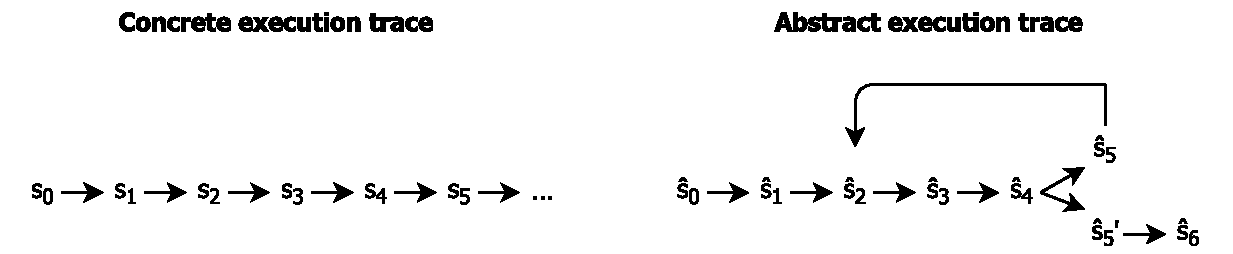
\includegraphics[width=1.0\textwidth]{images/abstractInterpretation} 
      \caption{Concrete and abstract program execution traces}
    \label{fig:abstractInterpretation}
\end{figure}

\end{exmp}

%\subsection{Mathematical background}
%\label{subsec:lattice}

%In this, we look at the mathematical concepts that form the base of abstract interpretation. The concepts defined in this section will aid us in formally defining an \textit{abstraction}. This definition is needed to understand how precision loss is caused by abstracting values.

%\begin{definition}
%\textit{A relation $\sqsubseteq: S \times S$ is a \textbf{partial order} if it has the following characteristics:}
%\begin{enumerate}
%\item Reflexivity: $\forall x \in S : x \sqsubseteq x$
%\item Transitivity:  $\forall x,y,z \in S : x \sqsubseteq y \wedge y \sqsubseteq z \Rightarrow x \sqsubseteq z$
%\item Anti-symmetry: $\forall x,y \in S : x \sqsubseteq y \wedge y \sqsubseteq x \Rightarrow x = y$
%\end{enumerate}
%\end{definition}
%\begin{definition}
%\textit{A \textbf{partially ordered set} ($S$,$\sqsubseteq$) is a set with a partial order}
%\end{definition}
%\begin{definition}
%\textit{For a subset $X \subseteq S$, $u$ is an \textbf{upper bound} of $X$ if $u\in S, \forall x \in X: x \sqsubseteq u$. $u$ is the \textbf{least upper bound} of $X$ ($\bigsqcup X$) if for every upper bound $x$, $u \sqsubseteq x$. Similarly, the \textbf{lower bound} of $X$ can be defined as: $l \in S,\forall x \in X: l \sqsubseteq x$. $l$ is the \textbf{greatest lower bound} of $X$ ($\bigsqcap X$) if for every lower bound $x, x \sqsubseteq l$. Two important operators on partial orders are \textbf{join} ($\sqcup$) and \textbf{meet} ($\sqcap$). $x \sqcup y$ denotes $\bigsqcup\{x,y\}$, the least upper bound of $x$ and $y$, $x \sqcap y$ denotes $\bigsqcap\{x,y\}$, the greatest lower bound of $x$ and $y$.}
%Least upper bound
%\end{definition}

%\begin{definition}\label{def:lattice}
%\textit{A \textbf{lattice} $(L,\sqsubseteq)$ is a partially ordered set in which any two elements have a least upper bound and a greatest lower bound. A \textbf{complete lattice} $(C,\sqsubseteq)$ is a partially ordered set in which all subsets have a least upper bound and a greatest upper bound. A complete lattice includes two special elements: a \textbf{bottom} element $\bot = \bigsqcap C$ and a \textbf{top} element $\top = \bigsqcup C$.}
%\end{definition}

%\begin{definition}
%\textit{A \textbf{Galois connection} is a particular correspondence between two partially ordered sets $(A\sqsubseteq_A)$ and $(B\sqsubseteq_B)$. More precisely this correspondence is a pair of functions: the \textbf{abstraction function} $\alpha : A \rightarrow B$ and the \textbf{concretization function} $\gamma : B \rightarrow A$, such that $\forall a \in A, b \in B: \alpha(a) \sqsubseteq_B b \Leftrightarrow a \sqsubseteq_A \gamma(b)$.}
%\end{definition}

%TODO: lattice voorbeeld
\begin{figure}
% center everything in the figure
\centering
% horizontal node distance
\begin{tikzpicture}[node distance=2cm]

\title{Partially ordered set of signs (complete lattice)}
\node(TOP)                          			 {$\top$};
\node(PLUS)     [below right=.6cm and .6cm of TOP] {$+$};
\node(ZERO)     [below=.6cm of TOP]       		 {$0$};
\node(MINUS)    [left=.6cm of ZERO]       		 {$-$};
\node(BOT)     	[below=1.8cm of TOP] {$\bot$};
\draw(TOP)      -- (PLUS);
\draw(TOP)      -- (ZERO);
\draw(TOP)      -- (MINUS);
\draw(BOT)      -- (PLUS);
\draw(BOT)      -- (ZERO);
\draw(BOT)      -- (MINUS);
\end{tikzpicture}
\caption{Partially ordered set of signs (complete lattice)}
\label{fig:lattice}
\end{figure}

\subsection{Abstraction}
An \textit{abstraction} $\hat{X}$ of a concrete set $X$ in abstract interpretation is a Galois connection between the power set of $X$ $(\mathcal{P}(X),\subseteq)$ and $X$ itself $(X,\sqsubseteq)$. The abstraction function $\alpha$ maps a concrete value to its abstract counterpart, whereas the concretization $\gamma$ function maps an abstract value to its concrete counterpart\textit{s}. Abstract values, sets and operations are generally indicated with a hat. Example \ref{ex:signAbs} illustrates how abstraction works, and how it causes \textit{imprecision} to occur.

\begin{exmp} 
\label{ex:signAbs}
(Sign abstraction). A possible abstraction of integers $\mathbb{Z}$ could be to map them onto the set of signs $\widehat{Sign}$. The set of signs forms a complete lattice with $\sqsubseteq$ ordering, as depicted in figure \ref{fig:lattice}. This abstraction could be used in an analysis to detect divisions by zero, for example. We can define the abstract and concretization functions as follows:\\


\centerline{$\alpha:\mathcal{P}(\mathbb{Z}) \rightarrow \widehat{Sign}$}
\centerline{$\alpha(Z) = \bot$ when $Z = \varnothing$}
\begin{addmargin}[5.84cm]{1em}% 1em left, 2em right
$= 0$ when $Z = \{0\}$\\
$= +$ when $\forall z \in Z, z > 0$\\
$= -$ when $\forall z \in Z, z < 0$\\
$= \top$ otherwise
\end{addmargin}
\leavevmode \\\\
\centerline{$\gamma:\widehat{Sign} \rightarrow \mathcal{P}(\mathbb{Z})$}
\centerline{$\gamma(P) = \varnothing$ when $P = \bot$}
\begin{addmargin}[5.84cm]{1em}% 1em left, 2em right
$= {0}$ when $P = \hat{0}$\\
$= \mathbb{Z}^+$ when $P = +$\\
$= \mathbb{Z}^-$ when $P = -$\\
$= \mathbb{Z}$ otherwise\\
\end{addmargin}
\leavevmode \\
The addition operator $+$: $\mathbb{Z}\times\mathbb{Z}\rightarrow\mathbb{Z}$ can also be abstracted to $\hat{+}$: $\hat{\mathbb{Z}}\times\hat{\mathbb{Z}}\rightarrow\hat{\mathbb{Z}}$ following the rules of sign. Some examples:\\


\centerline{$\{0\}  \hat{+}  \{+\} = \{+\}$}
\centerline{$\{-\}  \hat{+}  \{-\} = \{-\}$}
\leavevmode \\
but for more advanced examples, we can easily see a loss in precision:\\\\
\centerline{$\{+\}  \hat{+}  \{-\} = \{-,0,+\}$}
\centerline{$\{0\}  \hat{+}  \{0,+\} = \{0,+\}$}
\\\\
When applying the concretization function after the abstraction function, we observe that the result is less precise. Consider the negation function $f(N) = \{-n \vert n \in N\}$, which negates an integer. Applying the concretization function to an integer directly results in no loss of precision:\\ 
\centerline{$f(\{1\}) = \{-1\}$,}\\ whereas applying it after the application of the abstraction function overapproximates the concrete value: \\
\centerline{$(\gamma \circ f \circ \alpha)(\{1\}) = \mathbb{Z}^+$}\\
$\mathbb{Z}^+$ is an overapproximation of $\{1\}$, conserving all properties that hold for $\{1\}$. The closer something is abstracted to its concrete value, the higher the precision of the analysis will be.
\end{exmp}

%To conclude this section, we briefly discuss why this loss of precision is important for this dissertation. When calculating value flow by performing static analysis through abstract interpretation, precision is also lost. In most programming languages, variables and objects point to values and addresses respectively. It is obvious to see that simple calculations lose precision as in the example above. As a result of abstract interpretation, multiple addresses may point to the same object. This is exactly the kind of imprecision that is introduced in the analysis that is used in this dissertation. As each of these addresses is as valid of an address as any other, we need to consider all addresses of matched variables/objects on all matched paths in the state graph.

\section{Support for generic vulnerabilities}
\label{sec:genericVulnerabilities}

Static analysis is often used by model checkers to verify if a program satisfies a set of properties (i.e. a specification of a program). These tools usually require additional information to be added to the program before being able to analyze it. The OWASP LAPSE+ plugin for Eclipse~\cite{OWASP:LAPSE} for example requires the user to annotate all possible vulnerability sources and sinks in the source code. It then checks if there is information flow between a source and a sink. 

\subsection{Limitations}
Although applicable to many programs, tools for finding general characteristics of programs is limited in several ways:
\begin{enumerate}
\item The set of problems that these tools can detect is often restricted and a lot of tools support detection for similar problems. Tools detecting bug patterns detect only the patterns that are pre-encoded in the tool. This implies that the tool only supports bug patterns that are pre-encoded and thus will most likely miss any bug pattern that isn't already encoded. 
\item Poorly encoded patterns may miss bugs, making the analysis of the tool unsound. 
\item Adding or extending functionality to existing solutions is often cumbersome and in most cases even impossible to do manually, which makes these solutions less useful for certain domain-specific programs, as these require a flexible tool. 
\end{enumerate}

To remedy these problems, a more practical approach would be to develop a tool which allows users to define by themselves what they wish to detect in a program. This approach would make the analysis \textit{application-specific} and the detection rules would be \textit{user-defined}. More about application-specific approaches can be found in section \ref{sec:applicationSpecificVulnerabilities}. 


\subsection{Existing analysis tools}

The remainder of this section discusses the most popular static analysis approaches for model checking and finding generic code characteristics and vulnerabilities.
\subsubsection*{JOANA}
The Java Object-Sensitive Analysis project (JOANA~\cite{JOANA}) is an Eclipse plugin which checks for security leaks in Java programs. The tool supports all Java language features (except for reflection) and scales well for larger programs. The analysis used is flow-sensitive, context-sensitive, object-sensitive and lock-sensitive, minimizing the amount of false positives drastically. The types of security flaws JOANA is able to detect are:
\begin{enumerate}
\item \textit{Confidentiality}: Information about sensitive values, like passwords or personal data, should in no case be conveyed to public outputs.
\item \textit{Integrity}: The dual of confidentiality: In no way should unsafe program inputs alter secure data or influence sensitive computations of a program.
\end{enumerate}
These flaws are detected by creating a system dependence graph (SDG) of the program on which information flow between sources and sinks is checked through program slicing. The SDG is an overapproximation of the information flow through the program. A benefit of this kind of graph is that it is able to detect direct (data) as well as indirect (control) dependencies. In order for the analysis to run, the user has to specify which parts of a program should act as sources and which should acts as sinks. This is done by adding annotations to the source code. JOANA comes with a machine-checked soundness proof. Although JOANA is capable of finding dependencies between program points, it is limited in the amount of vulnerabilities it detects and there is no way to extend the tool to support more vulnerabilities.

\subsubsection*{Flawfinder}
Flawfinder\footnote{http://www.dwheeler.com/flawfinder} is a tool for examining C/C++ source code and detecting security weaknesses. It comes with a database of well-known problems, such as buffer overflow risks and race conditions. The results of the performed analysis is a report of all found flaws with a corresponding security risk level. Although being useful to quickly check for security vulnerabilities, Flawfinder is not extensible and it is not aware of the semantics of the system under test. Control flow and data flow analysis are not supported by the tool, making it a naive approach.

\subsubsection*{FindBugs}

FindBugs~\cite{Findbugs} is a static analysis tool for detecting bugs in Java programs. It detects many classes of bugs by checking structural bug patterns against a program's source code. These classes of bugs can be subdivided into three main classes: correctness bugs, dodgy confusing code, and bad practices. Recently, the Find Security Bugs plugin\footnote{http://find-sec-bugs.github.io} was developed on top of Findbugs. This plugin can detect 80 different (pre-encoded) vulnerability types, among which are the top 10 OWASP security vulnerabilities. An example security violation detected by the plugin is the parsing of an untrusted XML file. The contents of this file might be malicious and thus may pose as a risk for the application. As the plugin is able to detect a wide range of bugs, the tool is well-suited to check for the most common security vulnerabilities. Nevertheless, only those vulnerabilities can be detected, and when a new class of security violations arises, there is no way to add detection rules for these vulnerabilities as a regular user.

\subsubsection*{CodeSonar}
CodeSonar~\cite{CodeSonar}, developed by GrammaTech, is a proprietary source code analysis tool that performs a unified data flow and symbolic execution analysis for C, C++ and Java programs. GrammaTech claims to detect more code flaws than the average static analysis tool because they do not rely on pattern matching or other similar approximations. The approach CodeSonar uses is to compile source code and generate several intermediate representations, such as control flow graphs, call graphs and AST's. The tool then traverses/queries these models to find particular properties or patterns that indicate defects. Next to performing general checks, CodeSonar provides an C API which gives developers access to its intermediate representations of the compiled program. A user can then define custom checks on these representations. We dit not verify the ease of use of these custom checks as we did not find any examples. The hybrid approach of CodeSonar (general checks \textit{and} application-specified checks) preludes the next section of this chapter, which discusses approaches that support detecting application-specific vulnerabilities through user-defined queries and rules.


\section{Support for application-specific vulnerabilities}
\label{sec:applicationSpecificVulnerabilities}

An often encountered problem with tools supporting detection of generic vunerabilities is that they often do not allow users to write their own rule or queries to find domain- and/or application-specific flaws. Even if some mechanism for specifying user-defined rules is available, as in PMD\footnote{https://pmd.github.io} for example, it often is cumbersome to write them in the tool's input language. These limitations makes that these tools are often not very flexible, and it makes it hard to extend them. 

In this section we discuss how putting the detection of application-specific characteristics and vulnerabilities in the hands of the application developer can facilitate the debugging process, by presenting some approaches which allow users to define their own program queries. Two main considerations for creating such a tool are (i) the way a program is represented and (ii) how the user is given access to this representation. The discussed approaches each have their own techniques to do so, and we elaborate on their advantages and disadvantages.


\subsubsection*{PQL}

The purpose of the PQL language is to check if a program conforms to certain program design rules~\cite{PQL}. More precisely, it can be used to check the presence of sequences of events associated with a set of related objects. The language allows programmers to query for these types of sequences in an application-specific way, rendering it useful to detect design defects on a per application basis.

Either dynamic or static analysis can be used to solve these PQL queries, but only the latter is of interest for this dissertation. The static analyser uses a context-sensitive, flow-insensitive, inclusion-based pointer analysis. As PQL attempts to optimize results of the static analysis to use them in the dynamic analysis, the used analysis must be sound. The points-to information, together with the program representation, is stored as a collection ofdatalog rules in a deductive database called \textit{bddbddb}. This is similar to the approach of GateKeeper~\cite{GateKeeper}.

Two interesting features of the PQL language are the support for subqueries and the ability to react to a match. The latter is only useful in the case we use dynamic analysis. Subqueries however add significant power to a language. In the case of PQL, they allow users to specify recursive event sequences of recursive object relations.

The actual matching of queries to these rules happens by first translating the PQL queries to the corresponding datalog queries. Once translated, the queries get resolved by the \textit{bddbddb} system, after which the results are ready to be interpreted by the user. Since the analysis used is flow-insensitive, sequencing is not supported in such a way that the user can distinguish whether program point \texttt{a} happens before or after program point \texttt{b}. The same holds true for negation: no guarantees about ordering can be made, which means that one can not deduce whether an excluded event (i.e. a negated event) happens between two points in a sequence. Therefore, in order to maintain soundness of the approach, all excluded events are ignored.

A benefit of using Datalog is that it is very efficient and has way less overhead compared to full-fledged declarative programming languages. Storing an analysis/program as datalog rules may be efficient, but it is hard to get a good overview of the program by just looking at these rules. PQL closes the gap between the lack in readability of plain datalog rules and writing clean application-specific queries by introducing its own language. However, this language is verbose and the syntax is something the user has to get used to.

\subsubsection*{Pidgin}

Pidgin~\cite{PidginQL} is a program analysis and understanding tool which allows users to specify and enforce application-specific security guarantees. The approach generates a \textit{Program Dependence Graph} (PDG) of programs by using an interprocedural data flow analysis (object-sensitive pointer analysis). This graph contains all information about how data data flows through a program. More precisely, each pair of connected nodes indicates that the second node of the pair depends in some way on the first node. Figure \ref{fig:PDG} shows a PDG of a guessing game.

\begin{figure}[!ht]
    \centering
      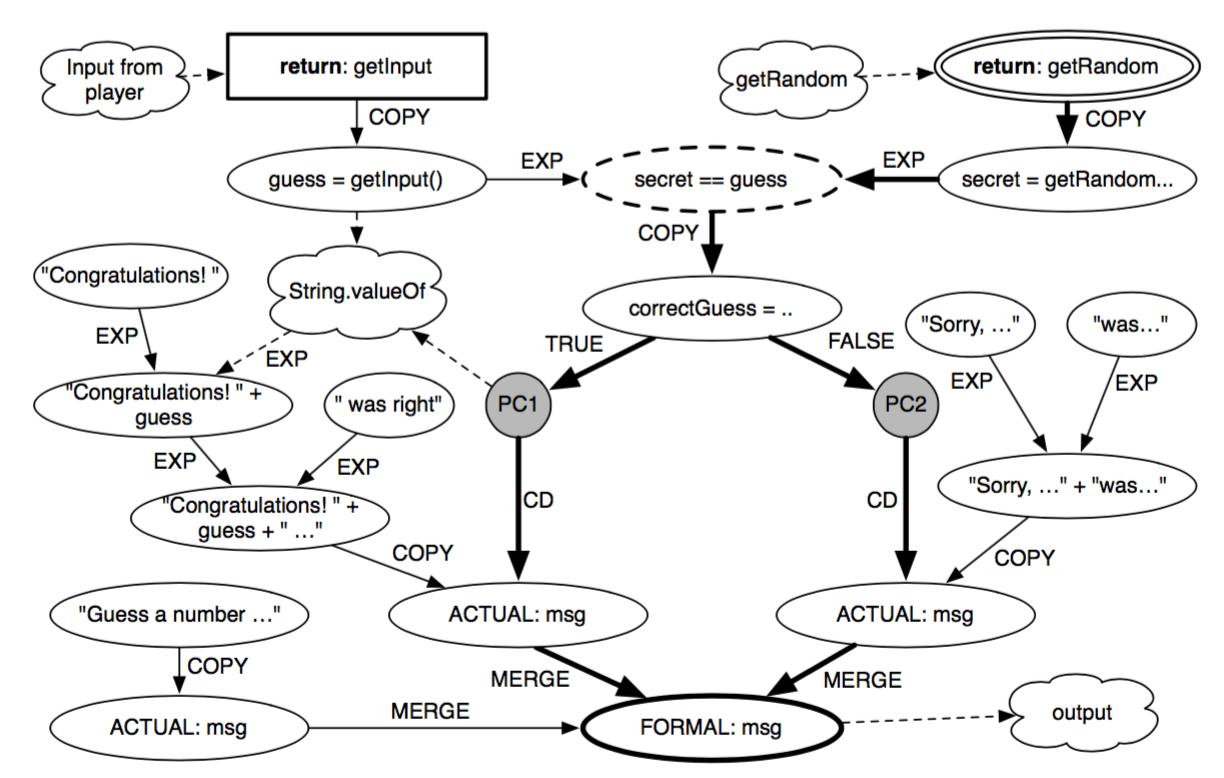
\includegraphics[width=0.7\textwidth]{images/PDG} 
      \caption{Program dependence graph of a guessing game}
    \label{fig:PDG}
\end{figure}

We can see that the value that flows to the output function indirectly depends on the value of the secret. This behaviour is usally undesirable, as information about the secret can be leaked to the output. This can be seen as a security violation and can be queried for in the Pigdin language. To this extent, the Pidgin Query Language (PidginQL) defines specialized constructs that allow the user to retrieve all relevant information from the PDG. As the program is represented as a graph, the approach specializes in detecting if there is information flow from one node to another. An example of a PidginQL query is seen in listing \ref{lst:PidginExample}. The usual approach to writing queries is as follows: 

\begin{enumerate}
\item Specify the nodes between which information flow (from \textit{source} to \textit{sink}) needs to be detected and store them in variables. A \textit{source} is a point in the program where sensitive information is available, whereas a \textit{sink} is a program point where information may exit the program. This is done through the aforementioned constructs.
\item Specify \textit{declassifier nodes}. These nodes act as sanitizers in a way that when information flows between a source and a sink and this information also flows through a sanitizer, then the flow is allowed.
\item Remove all declassifier nodes from the graph to make sure that the query won't detect false positives (i.e. no flows from source to sink through a declassifier node).
\item Check if there is any flow left between the specified sources and sinks.
\end{enumerate}

\begin{lstlisting}[label={lst:PidginExample},language=JavaScript,caption=A typical PidginQL query,mathescape=true]  % float=t?

//source, sink and declassifier
let source = pgm.returnsOf("getRandom") in 			
let sink = pgm.formalsOf("output") in 				
let declassifier = pgm.forExpression("secret == guess") in
//Remove declassifiers and check for flow
pgm.removeNodes(declassifier).between(source, sink)	 		
is empty											
\end{lstlisting}

The PidginQL language is expressive and powerful for detecting information flows. The language however lacks expressiveness when it comes to inspecting nodes. There are no constructs that allow the user to only find nodes with a certain name, for example. A second limitation is the result of queries. Most static analysis tools report all found violations, with more information about the violating code. PidginQL on the other hand just indicates whether there is flow or not (the \texttt{is empty} construct on line 7).

\subsubsection*{Metal}

Metal~\cite{Metal} is a general analysis tool of programs for which a user has to write application-specific extensions called checkers. These extentions are then executed as a traditional dataflow analysis, but can be augmented in ways which are usually not supported by other more traditional approaches. Metal extensions are applied depth-first to the control-flow graph of a function. This flow graph is computed from the AST of the program. By applying an extension depth-first, each program point down a single path in the graph is checked. This process is similar to pattern matching. Checkers in the Metal language consist of two parts: the actual code that describes the checker and a corresponding state machine. Metal distinguish two types of state machines: \textit{Global} state machines and \textit{variable-specific} state machines. The former is used for program-wide properties, whereas the latter detects object-specific properties. 

Checkers are written by defining states between which the state machine can transition. When the current program point matches a pattern described in the current state of the checker, the state machine transitions to the next state and/or performs an action (usually printing a warning). When there is no match for the current program point, the state machine does not transition and the analysis continues with the next program point. Example \ref{ex:Metal} clarifies the approach. 
\begin{exmp}
\label{ex:Metal}
Figure \ref{fig:Metal} shows an global extension which checks for the double enabling of disabling of interrupts (\texttt{sti()} and \texttt{cli()} respectively). When enabling interrupts, the state machine transitions to the 'enabled' state. When enabling interrupts a second time, an error showing ``Double sti'' is printed. The same happens for disabling interrupts: when a user attempts to disable interrupts twice, or when the end of a path is reached when interrupts are still disabled (and thus the state machine is still in the 'disabled' state), an error will be printed.

\begin{figure}[h]
    \centering
      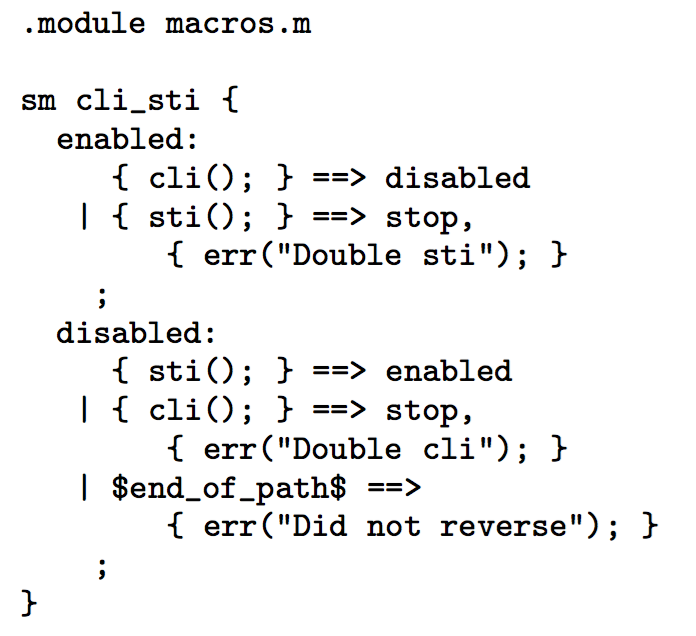
\includegraphics[width=0.4\textwidth]{images/Metal} 
      \caption{A simple double enabling/disabling checker}
    \label{fig:Metal}
\end{figure}

\end{exmp}

The Metal language is an example of a readable query language. Describing the states in the order one wishes to detect them is in our opinion the sweet spot in query languages combining power, expressiveness, flexibility and readability.

\subsubsection*{JunGL}

In contrast with other languages presented in this section, JunGL~\cite{JunGL} is a scripting language to perform \textit{refactorings}, based on pattern matching. Interesting in their approach is the specification of those parts of the code that need refactoring. In order to refactor some source code, the program first has to be represented in some way which is easy to access programmatically. JunGL does this by parsing the code into a uniform graph, initially containing only the information of the parsed AST. Lazy edges containing control flow information can also be added to the graph, but only when the refactoring needs this information. JunGL makes use of \textit{path queries} to express a pattern to be matched. 

For example, figure \ref{fig:JunGL} shows the path query to find the path from a variable occurence \texttt{var} to its declaration as a method parameter. This style of query denotation offers the exact amount of flexibility, readability and expressiveness needed to let developers express user-specified queries over a graph. An additional advantage of this type of queries is that no boilerplate code has to be written, as queries are self-contained.

\begin{figure}[!ht]
    \centering
      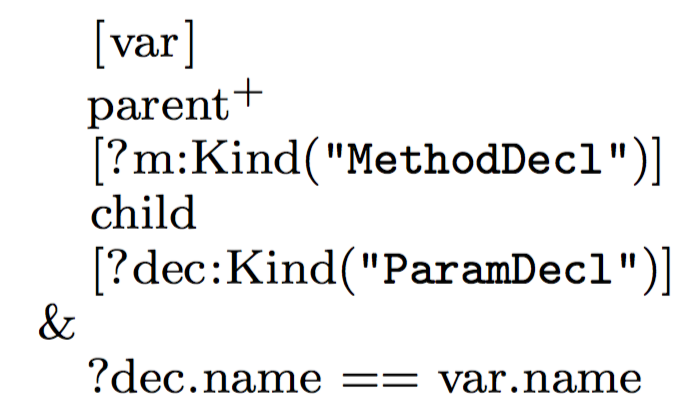
\includegraphics[width=0.4\textwidth]{images/JunGL} 
      \caption{A typical JunGL path query}
    \label{fig:JunGL}
\end{figure}

\section{Conclusion}
In this chapter we discussed what static analysis is and why it is important for detecting characteristics and vulnerabilities in source code. We have also discussed approaches that enable users to write clean and readable queries that define the patterns to be detected. From the discussion we conclude that the state of the art in static analysis has reached a point where tools supporting the detection of generic patterns often are not expressive and flexible enough for application-specific use. A solution to this problem is a tool and a language which allow users to specify their own, custom queries for an application. In this way, a database of pre-encoded vulnerability detection queries is not useful as the queries that are specified will mostly be too application-specific to generalize. We believe that expressing vulnerability queries (in the rest of this dissertation referred to as \textit{security policies}) is most readable and expressive using path expressions, as they they are close in form to a regular sentence consisting of consecutive pieces of code and states to be detected.


 
\chapter{Overview of the approach}
\label{ch:Overview}
\section{Architecture}

A program can be represented in several ways. There is extensive reading material on how logical programming can be used to represent and analyse programs\cite{Reps1995}\cite{DatalogDBQueries}. However, other approaches exist that lean more closely towards the implementation of our system.  As discussed in section \ref{subsec:staticAnalysis}, static analysis can be a means of representing implicit and explicit information about a piece of source code. For our approach, we needed a representation containing enough information to look up non-trivial properties about how information and data flows in the program. Abstract interpretation of a program produces an abstract state graph that meets these requirements. The graph contains information about control- and data flow, providing a rich source of information that can be extracted through some query language and a querying mechanism. 

% Querying mechanisms -> approaches in datalog queries enzo
Querying programs depends greatly on the way a program is represented and how queries are transformed into query-engine-friendly data structures. One way would be to resolve queries using existing techniques such as \cite{bddbddb}. This technique matches queries expressed in Datalog against a database of rules representing the relations of an entire program. Since our approach represents programs as flow graphs, an alternative method to resolve queries needs to be applied. A suitable algorithm to solving queries is presented in \cite{algoEngine}, which enables us to query flow graphs directly. The internals of this algorithm will be discussed in greater detail in section \ref{subsec:matchingEngine}.

% DSL
It is important that exploring and accessing information of a flow graph happens in an easy and user-friendly way. We believe regular path expressions to be the most legible way to write clean and understandable queries. With the JS-QL language, we offer an internal domain-specific language specialized in expressing queries corresponding to sequences of states in the flow graph. 

The actual architecture of the JS-QL framework is depicted in figure \ref{fig:architecture}. The query engine takes as input (i) a flow graph and (ii) a query, written in the JS-QL language. The output will consist of tuples \texttt{<State, Substitutions>} for all paths on which a match for the query was found.

\begin{figure}
    \centering
      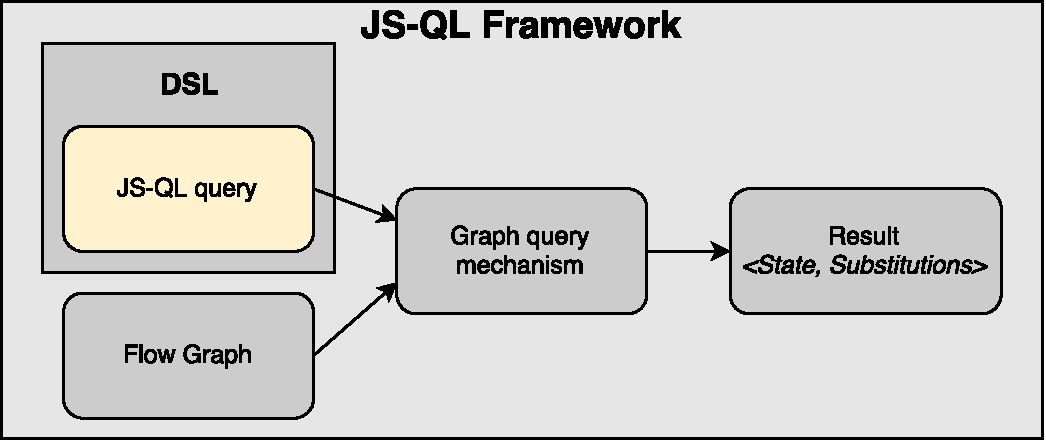
\includegraphics[width=0.9\textwidth]{images/Architecture} 
      \caption{JS-QL framework architecture}
    \label{fig:architecture}
\end{figure}
\section{Flow graphs for JavaScript programs}
\label{subsec:FlowGraphs}
The need for detailed control- and data flow information in our program representation graph limits the types of graphs that can be used for our framework. Program dependence graphs\cite{PDG} for example can be very useful to track the flow of information between certain points in a program but often lack more general information about program states, making them less qualified to use as our main program representation. In contrast, the JIPDA\cite{functionPurity} abstract state graph, generated by statically analyzing source code through \textit{abstract interpretation}, contains all the information needed to precisely express patterns to be detected in a program. This section takes an in-depth look at the JIPDA abstract state graph and the information it holds in its states. Figure \ref{fig:JipdaGraph} shows part of a typical graph produced by JIPDA for a program containing a check for whether a number is equal to zero or not.

As can be observed, the graph depicts all possible paths a program can traverse. Since the analysis in JIPDA is flow-sensitive, it is guaranteed that a state \texttt{a} on some path in the graph occurs before a state \texttt{b} on the same path if state \texttt{a} occurs first before state \texttt{b} on the path. This makes reasoning about patterns in a program much easier, since no false positives will occur with regards to the order of execution of states. The graph produced by the JIPDA analysis is also a flow graph, and more precisely maintains information about two types of flows:

\begin{enumerate}
\item \textit{data flow}: Information about what values an expression may evaluate to.
\item \textit{Control flow}: Information about which functions can be applied at a call site.
\end{enumerate}

We need these kinds of information to be able to make correct assumptions at certain states in a program. Consider the expression \texttt{f(x)} for example. Function \texttt{f} will be the function that is invoked. The value of \texttt{f} however may depend on other operations that occur before this function call, such as another function call. Therefore it is important to know which function(s) \texttt{f} may refer to, illustrating the need of control and data flow.

\subsection*{States of an abstract state graph}

JIPDA internally uses Esprima\cite{Esprima} to parse JavaScript code and set up an abstract syntax tree (AST). This AST is the starting point for the analysis that JIPDA performs, hence information about the nodes from the AST is also contained in certain states in the resulting graph. The small-step semantics of a program are defined by an abstract machine that transitions between different states. The abstract machine is in eval-continuation style, indicating that a state is either an evaluation state or a continuation state. These states correspond to the states that can be seen in the abstract state graph. This graph is an alternation of four different types of states. These states are marked in red and are so-called \textit{evaluation states}. Other states are \textit{continuation states} (green), \textit{return states} (blue) and \textit{result states} (yellow). The states the machine can be in are described below:

\begin{figure}[!ht]
    \centering
      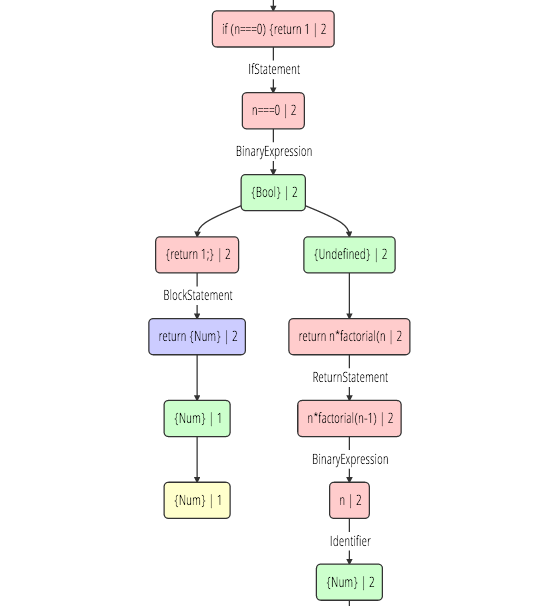
\includegraphics[width=262px, height=606px, keepaspectratio]{images/JipdaGraph} 
      \caption{Example JIPDA abstract state graph}
    \label{fig:JipdaGraph}
\end{figure}

%HELP VRAGEN BIJ JENS
\begin{enumerate}
\item \textit{Evaluation state}: Represents the evaluation of an expression of the program in the binding environment $\beta$.
\item \textit{Continuation state}: A state which indicates that the machine is ready to continue evaluation with the value it just calculated.
\item \textit{Return state}: This is a special kind of continuation state, as it indicates the return of a function application. When the machine is in this state it is ready to continue evaluation with the value calculated for the return of the function application.
\item \textit{Result state}: The final state of the graph, indicating the final computed value(s) of the program. This is also a special kind of continuation state. The machine and graph can have more than one result state, depending on the program's nature. 
\end{enumerate}

These states all contain valuable information about the point in the program they represent. The next part of this section discusses the different attributes that can be found in the states of the abstract state graph. 

%Kont, Lkont, Node, Benv, Store, Value
\subsection*{Node}

As said earlier, evaluation states contain information about the expression or statement they represent in the program. This information is stored in the form of an AST node, as obtained by the Esprima parser. Detailed information about the current expression or statement can be found in the properties of these nodes. Our approach makes extensive use of this information to find a match for a specified pattern along the graph. Note that node information is exclusively available in evaluation states. If we parse the following program \\\\
\texttt{function answerToTheUniverse(arg)\{}\\
\phantom{ }\phantom{ }\phantom{ }\phantom{ }\texttt{return 42;}\\
\texttt{\}}\\
\\
we obtain its corresponding JSON representation, listed in \ref{lst:EsprimaTree}.
\\
\begin{lstlisting}[label={lst:EsprimaTree},language=JSON,caption=Parsed JavaScript program AST, mathescape=true]  % float=t?

{
    "type": "Program",
    "body": [
        {
            "type": "FunctionDeclaration",
            "id": {
                "type": "Identifier",
                "name": "answerToTheUniverse"
            },
            "params": [
                {
                    "type": "Identifier",
                    "name": "arg"
                }
            ],
            "defaults": [],
            "body": {
                "type": "BlockStatement",
                "body": [
                    {
                        "type": "ReturnStatement",
                        "argument": {
                            "type": "Literal",
                            "value": 42,
                            "raw": "42"
                        }
                    }
                ]
            },
            "generator": false,
            "expression": false
        }
    ]
}
\end{lstlisting}

The parsed source code is a list of nodes contained in the body property of the "program" AST node. This is in fact the root node of the AST. Each node has its own \textit{type} that distinguishes different kinds of expressions and statements. The example code in \ref{lst:EsprimaTree} shows that the parsed code is a "FunctionDeclaration" with its own id, parameters, defaults and body attributes. We observe that the attributes in turn can again be (a list of) nodes.

\subsection*{Binding environment and store}

In JIPDA, variables point to addresses. The mapping of a variable to an address is called a \textit{binding}. These bindings reside in a \textit{binding environment} $\beta$. Each binding maps to a value through the \textit{store} $\sigma$. The store acts as a heap where bindings represent addresses on that heap. Being able to capture bindings, addresses and values in metavariables enables us to express and inspect data flow properties of programs. Variables are mapped to values in two stages. The first step for looking up a variable $\nu$ is to locate its binding in $\beta$. Next, the value of the variable can be looked up in the store by composing these two functions. The value of $\nu$ is given by $\sigma(\beta(\nu))$. This way of mapping variables to values allows us to reason about individual bindings, which is necessary because during interpretation multiple bindings to the same variable can exist simultaneously. Listing \ref{lst:benvStoreExample} gives an example of how a variable gets a binding and is later looked up.
\\
\begin{lstlisting}[label={lst:benvStoreExample},language=JavaScript,caption=Example of the binding environment and store workings, mathescape=true]  % float=t?

function f(){
  //$\beta$ contains a binding $x \rightarrow \widehat{Addr}$
  var x = 3; 
  
  //$\sigma$ has an entry $\widehat{Addr} \rightarrow \widehat{Val}$
  //and the (set of) corresponding value(s) for x is returned. 
  return x;
}
var value = f();
\end{lstlisting}


\subsection*{Value}
%Value uit store
The lookup of a variable through a binding in the store results in the (set of) value(s) for that variable. This information is available in all states but evaluation states. Values can either be addresses or undefined. For continuation states, the value will represent the looked up or calculated values of an expression. A return state's value is the set of possible values that will be returned. Result states contain the final values of a program.

\subsection*{Stack}

The stack is a local continuation delimited by a meta-continuation. The \textit{local continuation} is a (possibly empty) list of frames which acts as a stack (of frames), with normal push and pop functionalities. A \textit{meta-continuation} is either empty or a stack address pointing to the underlying stacks in the stack store. These stack addresses are generated at call sites and thus represent the application contexts. Useful information such as the call stack can be obtained by tracing out all reachable stack addresses in the stack store, starting from the context that is directly contained in the current state. The traversal of the stack terminates when we encounter an empty meta-continuation, also called the \textit{root context}. A program starts and terminates evaluation in this root context, provided that evaluation happens without errors. The root context corresponds to the top-level part of a program, the global namespace in JavaScript.

Although our framework doesn't provide stack traversal functionalities, basic properties of the stack (local continuation and meta-continuation) can be used and inspected to detect different kinds of states. For a function application, states corresponding with the start and end of the application will have the same local and meta-continuation. With this information, we can for example check for each path if there is a function application followed by a specific state \textit{before} the end of that function application. A concrete example of such a state is a recursive function call.

\section{External DSLs for querying graphs}

For almost any branch of science and engineering we can distinguish between two types of approaches. One type of approach is the \textit{generic} approach, which offers solutions to a wide range of problems within a certain domain. However, these solutions are often suboptimal. When we reduce the set of problems we want to solve, an often better approach to solving these problems would be the \textit{specific} approach.
In software engineering terms these two approaches translate to two types of languages: General purpose languages (GPLs) and domain-specific languages (DSLs) respectively. 
\textit{Domain-specific language} is no new concept. Many programming languages that are now considered general purpose language started out as domain-specific languages. Cobol, Fortran and Lisp for example all came into existence as dedicated languages for solving problems in a certain area\cite{vanDeursen:2000}, but gradually evolved into the full fledged languages they are today. The rest of this section is devoted to the comparison of GPLs and DSLs, in which we advocate that DSLs are the best approach for the instantiation of the JS-QL framework. We further give an overview of related work about DSLs for querying graphs.


\subsection{Domain-specific language vs. general purpose language}
\label{subsec:DSLvsGPL}

Before we start this comparison, we give a formal definition of domain-specific languages and general purpose languages:
\begin{definition}
    A \textit{domain-specific language} (DSL) is a programming language of executable specification language that offers, through approproate notations and abstractions, expressive power focused on, and usually restricted to, a particular problem domain.
\end{definition}

\begin{definition}
    A \textit{general purpose language} (GPL) is a programming language that is broadly applicable across application domains, and lacks specialized features for a particular domain.
\end{definition}

The key focus for DSLs are its focussed expressive power. The expressiveness of DSLs comes from the fact that they were created to solve a small set of problems. They offer a high-level set of mechanisms for the programmer to express his ideas for a particular application domain. A DSLs aim is to have the language focus specifically on those aspects and concepts that are relevant to a particular problem domain, hiding all boilerplate code that comes along with GPLs. Designers of general purpose programming languages also try to help the programmers express their ideas concisely and clear, but even with the most elegant programming language difficulties arise when programs get bigger and more complex. To this extent, extra features were developed for GPLs to further abstract code and reduce complexity. Amongst these features are functions, subroutines, packages, objects \dots  Even though these features are useful for general applications, the languages that implement them often have a set of operational baggage associated with them which makes a program unneccesarily complex to develop\cite{FluentInterfacesJava}. 

In contrast to the generic approach, the domain-specific approach to language design makes it possible to allow low-level system requirements to guide the design of the required high-level language features one wishes to incorporate into his language, instead of being required to use existing general-purpose designs.
We therefore believe that a domain-specific language is the best pick for our query language.
Benefits of domain-specific languages include:

\begin{itemize}
\item DSLs are application-specific. This allows users to express their ideas at the level of abstraction of the problem domain.
\item DSL programs are concise, self-documenting and highly reusable\cite{Bentley:1986}
\item Increased productivity: Once the language design and implementation have finished, work becomes much more efficient as you don't have to write the boilerplate code of the GPL manually. In this way you can replace a lot of GPL code with a few lines of DSL code.
\item Domain expert involvement: DSLs whose domain, abstractions and notations are closely aligned with how domain experts reason and express themselves, allow for a fluent integration between developers and domain experts. Domain experts can read, and possibly even write code in the language as they are not directly confronted with any implementation details.
\item Programs are often expressed at a level of abstraction that is meaningful for the domain. This brings along that these programs contain domain knowledge and that they can be reused with few to no modifications.
\item Improved code quality: Fewer bugs, better architectural conformance, increased maintainability. This is the result of the partially removing the programmers freedom and the avoidance of code duplication by providing DSL constructs.
\end{itemize}

\noindent Some counterarguments for using a DSL are:
\begin{itemize}
\item The cost of designing, implementing and maintaining a DSL
\item The cost of educating DSL users
\item A DSL has limited applicability
\item The difficulty of finding the correct scope for a DSL
\end{itemize}

We argue that the costs for setting up a DSL do not weigh up against the benefits of a DSL. The high reusability alone makes up for the one-time investment of designing and implementing the language. When developing a language for a certain domain, naturally its applicability will be limited to that domain only, as this is the purpose of a domain-specific language. Finding the correct scope for a DSL might be cumbersome, but there is a great amount of literature about specifying the domain of a problem\cite{Simos:1995} and the domain for DSLs\cite{karsai2014design}\cite{gunther2010agile}. 

\subsection{External DSLs}

Many DSLs come along with a compiler which translates DSL programs into applications. These kinds of DSLs are called \textit{external} DSLs. the compiler is also called an application generator\cite{Cleaveland:1988}, whereas the DSL is the application-specific language. The main advantage of external DSLs is that the implementation of the compiler can completely be tailored to the DSL. The DSL in turn is restricted in no way with regards to notation, primitives and the like because its syntax is independent of the underlying host language (since there is none). The remainder of this section discusses existing work about external DSLs used for graph traversal and graph querying.

\subsubsection*{StruQL}

StruQL is the query language behind the Strudel system\cite{Fernandez97aquery}. The language is built to support the retrieval and construction of data for web sites. This data is represented as \textit{data graphs} and originates from external sources, the integrated view and the web site itself. These data graphs depict web sites as nodes, representing web pages or atomic values, interconnected with directed, labelled edges. These edges then represent the links or attribute values that connect two nodes. The language enables users to create and query data graphs, but the real power of StruQL lies in their ability to express regular path expressions. This allows for very flexible queries describing the paths about which information needs to be accessed in great detail.
It also allows to compute the transitive closure of an \textit{arbitrary 2n-ary} relation, meaning that it can compute all reachable nodes from a certain node for any input graph. Buneman et al\cite{Buneman:1996} have formally proven that this is not a trivial computation.

\subsubsection*{GraphQL}
%http://sites.fas.harvard.edu/~cs265/papers/he-2008.pdf -> GraphQL

GraphQL\cite{He:2008} is a query language which allows to query graph databases. The language uses a graph pattern as a basic operational unit. These graph patterns consist of a graph structure and a predicate on attributes of the graph. They introduced the notion of formal languages for graphs. This is useful for composing and manipulating graph structures and is used as a basis of the graph query language.
The core of the language is a graph algebra in which the selection operator is generalized to graph pattern matching and a composition operator is introduced for rewriting matched graphs. In terms of expressive power, the language is contained in Datalog. This means that every query in GraphQL can be converted to a Datalog query. The language allows users to express concatenation, disjunction and recursion, allowing users to write dynamic queries. They address the NP-completeness of subgraph isomorphism by using neighborhood subgraphs and profiles, joint reduction of the search space, and optimization of the search order.

\subsubsection*{ASTLOG}
%http://www.cs.nyu.edu/~lharris/papers/crew.pdf
ASTLOG\cite{Crew:1997} is a query language for syntax-level C/C++ program analysis and is well suited to construct anchored patterns to match tree-like structures. The language is built as a Prolog variant syntax-wise, but instead of transforming an entire program into a database of Prolog rules, it is able to match \textit{objects} to queries directly. These objects are being made available through a C/C++ compiler frontend which provides an interface to the syntactic/semantic data structures build during the parse of a program. Among the available objects are the AST nodes of a program. These nodes can then be examined and queried by user-defined predicates in a similar fashion as one would do in Prolog. This allows for application-specific composable predicates. 

\subsubsection*{Lorel}
The Lorel language\cite{abiteboul1997lorel} was designed to query semistructured data. This kind of data can be seen as a graph with complex values at internal nodes, labeled edges and atomic leaves. The language's syntax resembles that of OQL (\textit{Object Query Language}), but has two two additional features: (i) A coercion mechanism for value/object comparisons and (ii) powerful path expressions. Coercion is needed for semistructured data, as two objects may represent the same data in different ways. Lorel introduces \textit{general path expressions}, a way to define label completion and regular expressions in paths. Regular expressions are supported through \texttt{.},\texttt{+},\texttt{?},\texttt{*},\texttt{()} and \texttt{|}, label completion is done as in SQL, namely with the \texttt{\%} symbol.
%http://infolab.stanford.edu/lore/pubs/lorel96.pdf -> Semistructured data

%-----------------------------
%RW over EDSL los van graphs:
%http://graphics.stanford.edu/hackliszt/liszt_sc2011.pdf
%http://homepages.cwi.nl/~jurgenv/papers/SCAM-2009.pdf
%https://www.researchgate.net/publication/220071161_BDL_A_Specialized_Language_for_Per-Object_Reactive_Control
%Chandra1999
%-----------------------------


\subsection{Internal DSLs}

In contrast to external DSLs, \textit{internal} (or \textit{embedded}\cite{Hudak:1996}) DSLs don't require a custom compiler. These languages inherit the infrastructure of some other (general purpose) language, and tailor it towards the domain of interest. In this way the language can be interpreted by its host language, saving the developer a lot of work. Although internal DSLs are restricted by the syntax of their host language, they can make full use of the host language as a sublanguage, thus offering the expressive power of the host language in addition to domain-specific expressive power of the DSL. This expressive power along with not having to build a fully fledged compiler for our DSL are the main reasons we prefer the internal DSL approach above the external DSL one. The rest of this section describes three internal DSLs, two for graph traversal and one that illustrates the flexibility and expressiveness of embedded DSLs. The terms internal DSL and embedded DSL both have the same meaning in the rest of this dissertation and both refer to the type of DSL that is embedded in a host language.

%Waarom internal
%----------------
%RW over DSEL graph traversal:
\subsubsection*{Gremlin}
%http://arxiv.org/pdf/1508.03843.pdf -> Graph traversal
\cite{Gremlin} presents the Gremlin graph traversal machine. The machine traverses graphs according to a user-specified traversal, making use of so-called traversers. These traversers can be seen as 'workers' who walk through the graph, keeping a bag of information on their back about the path they have already taken and the current graph node they are in. The machine is developed in such a way that it can be implemented as an embedded DSL in any host language, provided that the host language supports \textit{function composition} and \textit{functions functions as first-class entities}. The Gremlin language has an \textit{instruction set} of about 30 steps and each query is a sequence of these steps (i.e. a path). Querying graphs through paths is a well-known approach, but the Gremlin machine also supports nested paths for which each nested path is a graph traversal on it's own. Queries are transformed into traversals, so each traversal can be made application-specific. They present 9 different traversals, including a recursive and a domain-specific one. 

\subsubsection*{Dagoba}

Dagoba is an in-memory graph database system written in JavaScript. The chapter about Dagoba in the \textit{500 Lines or Less}\footnote{http://aosabook.org/en/500L} book provides an elaborate explanation on how to create a flexible, easily extensible internal DSL. The language is built as a fluent API, and explains which mechanics (such as lazy evaluation) go hand in hand with this kind of language representation. They also describe how they interpret the language and define some optimizations of the system, mainly through query transformators.

\subsubsection*{A little language for surveys}

A Little Language for Surveys \cite{RubyDSL} explores the use of the Ruby programming language to implement an internal domain-specific language. It checks how well the flexible and dynamic nature of the language accomodates for the implementation of a DSL for specifying and executing surveys. Two key features of the Ruby programming languages are exploited because they especially support defining internal DSLs: The flexibility of the syntax and the support for blocks. Function calls for example are easily readable, since the braces surrounding the arguments can be omitted and the arguments list can consist of a variable number of arguments (The latter is also supported in JavaScript\cite{Ecma6}). They make extensive use of the fact that entire blocks can be attached to method calls. These blocks are passed unevaluated to the called method, enabling \textit{deferred evaluation}. Next to these features, the meta-programming facilities of the Ruby makes it possible for them to read a DSL program and execute it in the contexts specified by that program. A two-pass architecture is used, splitting up the parsing and interpretation of the program. This is common practice for internal DSLs.

%Survey language -> illustrates flexibility of embedded dsl + design patterns
%
%-----------------------------
%RW over DSEL los van graphs:
%https://www.usenix.org/events/dsl99/full_papers/jennings/jennings.ps
%https://www.usenix.org/legacy/publications/library/proceedings/dsl97/full_papers/stevenson/stevenson.pdf
%http://haskell.cs.yale.edu/wp-content/uploads/2011/02/padl99.pdf
%Eliott1999
%https://www.usenix.org/legacy/publications/library/proceedings/dsl97/full_papers/kamin/kamin.pdf
%-----------------------------


\section{Design of an internal DSL for querying flow graphs}

%zie Domain-specific languages: An annotated Bibliography
Crafting a compiler for our languages falls outside the scope of this dissertation and we believe that the overhead for building an external DSL does not weigh up against the benefits of an internal DSL (as discussed in \ref{subsec:DSLvsGPL}).
In this section we discuss the design process of our internal domain-specific language named JS-QL.

\subsection{Internal DSL design constraints}

This section describe some factors that influenced the design of our query language. A first constraint for the language is that it was designed as an embedded DSL. This has as a consequence that we have to use the constructs and syntax the host language offers, JavaScript in our case. The JS-QL languages makes extensive use of JavaScript \texttt{Object}s that function as dictionaries. A limitation for us was that these dictionaries only accept strings as keys. Function calls for example can't serve as keys in JavaScript objects as their value can't always be calculated at compile time. This was a serious drawback for us and it even lead to an inconsistency in our language, as will be discussed in chapter \ref{ch:JSQL}. 
Our language has to be easily extensible as users need to be able to specify their own predicates and policies. To this extent, JavaScript surfaced as an ideal language. The dynamic typing and optional function arguments made creating flexible predicates and policies a lot easier.

Flow graphs need to be queried, so the language has to fit these needs in the form of appropriate predicates. The design of our language depended on the information that is contained in each state of the graph. The JIPDA graph states contain several fields that in turn can recursively contain other fields. The nature of the algorithm we use together with the structure of these states asked for a close mapping of states to query predicates. As JavaScript objects are great for storing nested information, we chose to use them as a mapping for states. From now on these objects will be referred to as \textit{dictionaries}. Fields in a dictionary now have a one-to-one relationship with fields in a state, making the matching process for the algorithm less of a burden. Another constraint imposed by the flow graph was that sequences of states had to be expressed in a precise yet legible fashion. This had as a result that the language was set up as a fluent interface, enabling the user to specify a number of states separated with a simple dot. We can thus say that the type of graph helped shape the JS-QL language.

%GEEN REPL
A final constraint was the need of an environment where queries can be expressed and evaluated against the flow graph. It would be tiresome to specify queries in one place and the input program elsewhere. This would also imply that every time a change to the program or the query has to be made, at least one separate file has to be modified. This is clearly not an optimal solution. As there is no \textbf{r}ead \textbf{e}val \textbf{p}rint \textbf{l}oop (REPL) available for JavaScript in the browser, we opted to extend the existing environment of the JIPDA analysis with support for (i) writing queries and (ii) checking these queries against the flow graph.


\subsection{DSL implementation techniques and patterns}

\begin{figure}[!h]
    \centering
      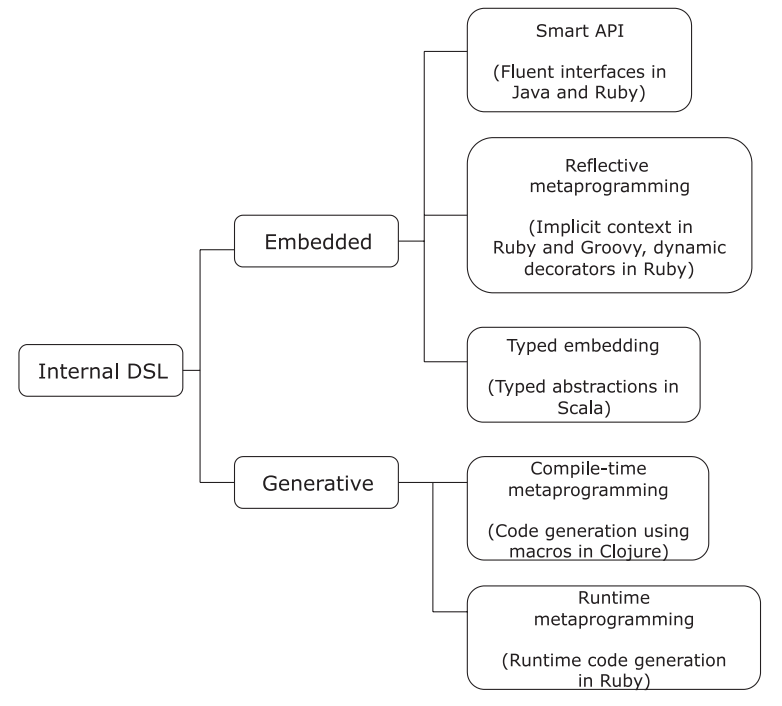
\includegraphics[width=0.8\textwidth]{images/DSLTechniques} 
      \caption{Internal DSL implementation techniques}
    \label{fig:DSLTechniques}
\end{figure}

Figure \ref{fig:DSLTechniques} shows the different kinds of implementation techniques for internal DSLs, as specified by \cite{Ghosh:2010}. Our DSL doesn't generate any code, so we won't discuss generative internal DSLs. Embedded internal DSLs on the other hand can be implemented in three ways: 

\begin{enumerate}
\item \textit{Smart API}: Readability is key for DSLs. Implementing a fluent interface is a way to improve readability and make Smart APIs. To this extend method chaining is a popular technique: It can be implemented by making the output of one method flow naturally as the input of another. Benefits are that a series of invocations in the DSL feel more natural and that it expresses the series of actions you want to perform or detect in the problem domain. Boilerplate code is not needed for this type of internal DSL, hence the name \textit{Smart} API.
\item \textit{Reflective metaprogramming}: The decorator pattern\footnote{https://en.wikipedia.org/wiki/Decorator\_pattern} is a well known pattern for extending individual objects. The ability to extend individual objects in a DSL greatly adds flexibility to the language. For some dynamically typed programming languages it is possible to define dynamic builders. These builders have a similar objective as the decorator pattern: construct an object incrementally within a DSL. This technique allows the language designer to smooth out the implementation aspect of the DSL by letting the user construct methods dynamically through the meta-object protocom of the language runtime.
\item \textit{Type embedding}: Types make for more concise and robust code. This is the philosophy that is behind the type embedding technique. Internal DSLs with a statically typed host language often use this pattern to make the language more expressive using the power of a type system. Each abstraction in the domain model should be made typed (and generic). This allows for fewer code duplication and a large part of the work will be done by the compiler of the host language. By making abstractions typed, correctness of programs written in the DSL is guaranteed: If the code compiles, it will most likely be correct.
\end{enumerate}

For our internal language we can already rule out the type embedding technique as JavaScript is a dynamically typed language. The problem domain of our approach doesn't need extra functionality to be added to individual objects in our language. These individual objects in our case are the states of the flow graph. States already are self-contained (they contain all necessary information) and don't require additional individual functionality. 

This leaves us with the smart API approach, which is ideal for our domain. By chaining methods in our DSL we can specify which states we want to encounter along the graph in a clearly specified order. Combining a smart API with several carefully chosen DSL design patterns\cite{DSLFowler} result in the concise and easily readable language that JS-QL is today. The remainder of this section elaborates on the chosen design patterns.

\subsubsection*{Method chaining}

Method chaining is the bread and butter of our DSL and at the same time also the \textit{only} way of expressing queries. This approach offers a fluent interface to the user in which it is hard to make any coding mistakes. The ability to express a state one wishes to encounter as a chained method to states he discovered earlier in the graph allows to build very readable queries. We illustrate this with an example: \texttt{G.skipZeroOrMore().functionCall()}. It is immediately obvious that this code is very intuitive: \texttt{G} is the entry point of our language, which indicates the start of a query. We then search for a path in the graph that contains a function call somewhere down that path. This is expressed by \texttt{skip}ping some, possibly none, states until a function call state is encountered.

\subsubsection*{Literal map}
%literal map
%-> Argument is a map similar to literal map
Specifying that one wishes to find states is often quite general. To this extent we need some sort of mechanism to express which types of states we want to match and what information we want to capture in (meta)variables. A literal map provides just this functionality by letting the user specify detailed key-value pairs. An example for could be: \texttt{.functionCall({name: 'f', arguments: '?args'})}. The literal map, enclosed in curly braces, indicates that only fuction calls with name \texttt{f} need to be matched and that the arguments of the matched state need to be captured in metavariable \texttt{?args}.

\subsubsection*{Object scoping}

The example for the method chaining design pattern is also applicable for the object scoping pattern. A single entry point \texttt{G} is created for queries, limiting the impact of the query that object. This pattern remedies two JavaScript flaws: Global namespace pollution and malicious code injection. This malicious code will only harm the \texttt{G} object, which is contained in some sort of sandbox.
%object scoping
%-> Alles wordt geevalueerd tegen 1 object om global namespace pollution tegen te gaan (alsook security issues)

\subsubsection*{Deferred evaluation}
%deferred evaluation
%-> Used to specify extra properties (not available at compile-time) + filters on values that aren't available
Some queries contain definitions for extra properties and filters. The information for these filters and properties is often not available at compile-time of our language. A mechanism is needed to delay the evaluation of those filters and properties until the matching process in the backend has collected enough information. Our framework handles this by creating thunks for filters and properties and unwrapping these thunks when the matching engine needs to evaluate them. By the time the evaluation happens, all variables should be bound in these thunks in previous matching steps. Consider a metavariable \texttt{?val} which captures the value of an assignment. If we only want to match assignment states with a value greater than 2, we have to create a thunk for the filter function \texttt{>} with arguments \texttt{?val} and \texttt{2}. We can't disregard states with \texttt{?val} greater than 2 immediately, as we don't know which value will be bound to \texttt{?val} at compile time.

\subsubsection*{Delimiter directed translation}
%delimiter directed translation
%-> Every method call is evaluated/parsed separately
Inherent to our DSL is delimiter directed translation. As method chaining is used as a means to set up our fluent interface, all methods are separated by a dot (the delimiter). Each method separated by this dot gets separately translated internally into a representation that is easier for our backend to process.

\subsubsection*{Newline separators}

Finally, the newline separators design pattern is incorporated in our DSL. This design pattern allows users to enter newlines between parts of their code. This greatly improves the readability and can split a program up in logical parts. Our DSL supports newlines in queries. This can be very useful to separate different states or sequences of states. Consider an example in which we only want to find assignments to variables \texttt{a} and \texttt{b}. Code can then be divided in two distinct parts, as in example \ref{lst:newlineSeparators}.

\begin{lstlisting}[label={lst:newlineSeparators},language=JavaScript,caption=Newline separators,mathescape=true]  % float=t?

.assign({leftName: 'a'}) //first logical part
.or()
.assign({leftName: 'b'}) //second logical part
\end{lstlisting}
%newline separators
%-> Language supports newlines between every state

%TODO conclusion?


\chapter{JS-QL: An internal DSL approach for querying flow graphs}
\label{ch:JSQL}
In this chapter we present the JS-QL framework. The framework offers the possibility for developers to write application-specific queries to check for certain program properties. More specific, it tries to offer a solution to developers who want to test their applications for vulnerabilities by writing and enforcing security policies for them. The framework consists of three main parts: 
\begin{enumerate}
\item \textit{The JS-QL query language}: Short for \textbf{J}ava\textbf{S}cript \textbf{Q}uery \textbf{L}anguage. This is the domain-specific language in which users can express all kinds of security policies. An overview of the language is given in section \ref{sec:JSQLlanguage}.
\item \textit{The matching engine}: This is the core of the framework. It matches the user-defined query against states of the JIPDA abstract state graph, capturing and unifying all the relevant information. This engine can be configured to behave differently for certain queries, as will be discussed in section \ref{subsec:TypesOfQueries}.
\item \textit{The graphical user interface}: The user interface provides the infrastructure for the developer to interact with the framework. It contains a section where users can specify the input program and security policy, a graphical component representing the abstract state graph corresponding to the input program and a visual and textual representation of the query results. The textual representation allows developers to inspect the captured variables, a handy feature when these variables are compound data structures. A brief overview of the user interface will be given in section \ref{sec:GUI}.
\end{enumerate}

\section{The JS-QL query language}
\label{sec:JSQLlanguage}

The abstract state graph obtained from the JIPDA analysis is a perfect starting point to inspect a program for certain characteristics and security vulnerabilities. In chapter \ref{ch:Overview} we motivated our choise to design an internal DSL to query for specific (sequences of) states in this graph, with the aim to discover program patterns that might lead to violations of user-defined security policies. The language constructs are built to make it easy for the user to specify which kind of pattern he wishes to detect. The rest of this section presents all facets of the JS-QL language: Section \ref{subsec:Syntax} discusses all constructs of the language and gives an in-depth explanation on how to use them in a correct way. As different security policies require different traversals of the state graph, more than one type of query is needed. We discuss the difference between several query types in section \ref{subsec:TypesOfQueries}. In order to have an effective query language, we must allow the user to create compound queries out of the available language constructs. Section \ref{subsec:DefiningPolicies} shows how this can be done within the framework.

\subsection{JS-QL syntax}
\label{subsec:Syntax}
 In this section we will discuss the available constructs and syntax of the JS-QL language. The examples in this section will be simplistic and will demonstrate how each construct works. They will therefore not always represent an actual security policy, but will rather serve as a guideline for using these constructs. We chose to use \textit{path expressions} to express queries in JS-QL, and more precisely \textit{regular path expressions}. This adds the flexibility of regular expressions to the language, as the most relevant features of regular expressions are incorporated in JS-QL.

%Entry point
\subsubsection{The entry point}
As our language is an internal DSL, meaning that it is embedded in a host language, the host language has to provide an entry point from where we can start using the JS-QL language. We chose to map this point to the \texttt{G} object, which is short for \textbf{G}raph. This implies that all query patterns in JS-QL will start from this object. A simple example is seen in \ref{lst:entryPoint}, where the first state of the graph is matched.

\begin{lstlisting}[label={lst:entryPoint},language=JSQL,caption=Matching the first state starting from entry point \texttt{G},mathescape=true]  % float=t?

//Match the first state of the graph
G.state()
\end{lstlisting}

\subsubsection{State}
the \texttt{state} construct is the single most basic element of the language. It matches any state in the graph, but doesn't provide much information on its own. Nevertheless is it the most important building block of the language, as it can be used to construct higher-level queries and predicates. States can be made more precise and expressive by parametrizing them with \textit{state constraints}, but in order to know what we can query for, we will first give a short overview of what information is available in which states. To get a more detailed explanation on what each piece of information represents, we refer to the section about flow graphs (\ref{subsec:FlowGraphs}). Table \ref{tab:InfoPerState} indicates what information is available in which type of state. The table also shows which keyword is used to represent the information is that is in embodied in the states.

\begin{table}[!h]
\centering
\caption*{
  \centering
  	\begin{tabular}{| l | c |}
  	\hline
  	\multicolumn{2}{ |c| }{Legend} \\
  	\hline
  	Evaluation state & $E$  \\
  	Continuation state & $K$  \\
  	Return state & $R_t$  \\
  	Result state & $R_s$  \\
  	All states & $A$  \\
  	\hline
  	\end{tabular}
  	%$E$ = EvalState, $K$ = KontState, $R_t$ = ReturnState, $R_s$ = ResultState, $A$ = All states
  }
  \begin{tabular}{| l | l | c |}
  \hline
  State property & Available in states & Keyword\\
  \hline
  Node & $E$ & node\\
  Meta continuation & $A$ & kont\\
  Local continuation & $A$ & lkont\\
  Binding environment & $E$ & benv\\
  Store & $A$ & store\\
  Value & $K$ $R_t$ $R_s$ & value\\ \hline \hline
  Identifier & $A$ & \_id\\
  Successors & $A$ & \_successors \\
  \hline

  \end{tabular}
  
  \caption{Information in the states of the abstract state graph}
  \label{tab:InfoPerState}
\end{table}

As readability is key in a query language, JS-QL provides four extra constructs that are semantically almost equivalent to the regular \texttt{state} construct. \texttt{evalState}, \texttt{kontState}, \texttt{returnState} and \texttt{resultState} are included in the language, with the purpose of enhancing readability, but also to match only those specific kinds of states.
Note that the framework also supports the usage of the identifier and successors of a state, but it is very uncommon to use them, as they are semantically irrelevant to queries. The identifier of a state would only be relevant when a query is matched in that exact state. When this is the case, the state gets marked in the visual graph representation and all query information is then contained in that state. To retrieve the information, one simply has to click the state to inspect all variable values. Successors also contain few additional information, as all direct successors of a state are already made explicit in the state graph. A use case for the use of the successors keyword could be to find all states after which some branching occurs. This could then be specified as a JS-QL query which captures the successors array in a variable \texttt{?succArr}, and then filters the results to only contain the states with the length of \texttt{?succArr} strictly greater than 1.


To understand how we can parametrize states, we first have to know how to define variables in JS-QL. Variables in JS-QL are strings, starting with a \texttt{?}. The fact that we use strings comes from the embedded nature of our language: If we were to specify variables as literals, the host language would complaint that it doesn't recognize the literal. Listing \ref{lst:stringVariables} illustrates this.

\begin{lstlisting}[label={lst:stringVariables},language=JSQL,caption=Defining variables in JS-QL,mathescape=true]  % float=t?

//Capture the 'type' property of the node in variable '?nType'
G.state({ node : { type: '?nType' }})
//Exception: ?nType is not recognized by the host language
G.state({ node : { type: ?nType }}) 
\end{lstlisting}

As the example might already indicate, JS-QL deconstructs state properties as nested key-value pairs. In this way, each part of information can be captured in a variable. The key indicates the property the user wishes to match whereas the value can be one of three things:
\begin{enumerate}
\item A \textit{variable}. When placing a variable as the value in a key-value pair in JS-QL, that variable gets bound to the key's corresponding value in the JIPDA state. The '?nType' variable in the example above gets bound to the value of \texttt{type}, which in this case corresponds with the type of the AST \texttt{node} for the currently matched state.
\item A \textit{nested map} which further deconstructs the current property. The example above does this by further deconstructing the \texttt{node} property of a state (which represents the corresponding AST node) in order to reach the \texttt{type} of that node and store it in a variable. It is obvious that this is most used to match specific AST nodes.
\item A \textit{literal}. Literals are mostly used to filter the states to be matched. When applying this to the example above, the '?nType' variable could be replaced by the literal 'ExpressionStatement' for example. Note that the question mark (\texttt{?}) is omitted. The resulting query would then only match a state having the \texttt{type} of its corresponding AST \texttt{node} equal to 'ExpressionStatement'.
\end{enumerate}

%Kort door de bocht?
\noindent States can thus be parametrized by matching the keywords displayed in table \ref{tab:InfoPerState} as keys with values that can be variables, literals or nested maps. It is obvious that queries matching single-state patterns aren't quite qualified as being security policies. JS-QL therefore allows users to specify sequences of states as a query. When checking the state graph against this query, all states in the query pattern need to be matched one after another. When a state in the query pattern is encountered that doesn't match the current state in the state graph, the matching process is aborted for the current path that is investigated in the state graph. Consider the following query:

\begin{lstlisting}[label={lst:Unification},language=JSQL,caption=Unification in JS-QL,mathescape=true]  % float=t?

G.state({ node : { type: '?tpe' }})
 .state({ node : { type: '?tpe' }})
\end{lstlisting}

\noindent We immediately see that the variable \texttt{?tpe} occurs twice in the query. This can be done on purpose to achieve \textit{unification}. Unification simply means that two variables with the same name have to contain the same value. After executiong the first line, the first state in the graph is matched (if it has the \texttt{node} property) and the variable \texttt{?tpe} is bound to the type of the node. The matching engine then proceeds to the next state in both the query and the state graph. If the next state again has the \texttt{node} property with the same type as already bound to \texttt{tpe}, the unification process has succeeded and the whole query will match. If the node type of the next state isn't equal to the value already bound to \texttt{?tpe}, or if that state doesn't have a \texttt{node} property, there is no match. The results of a successfully matched query will be the set of all possible \textit{substitutions}, together with the identifier of the state where the last element of the query matched. Figure \ref{fig:Unification} gives a simplistic visual representation of this process for the query listed in listing \ref{lst:Unification}. For the graph on the left-hand side, the query is fully matched by successfully unifying the the type of the first and second state. In contrast, the graph on the right-hand side will not produce a match as $\{$\texttt{?tpe} $:$ 'ExpressionStatement'$\}$ can't'be unified with $\{$\texttt{?tpe} $:$ 'AssignExpression'$\}$. More complex examples of unification can be found later in this chapter.

\begin{figure}[!h]
    \centering
      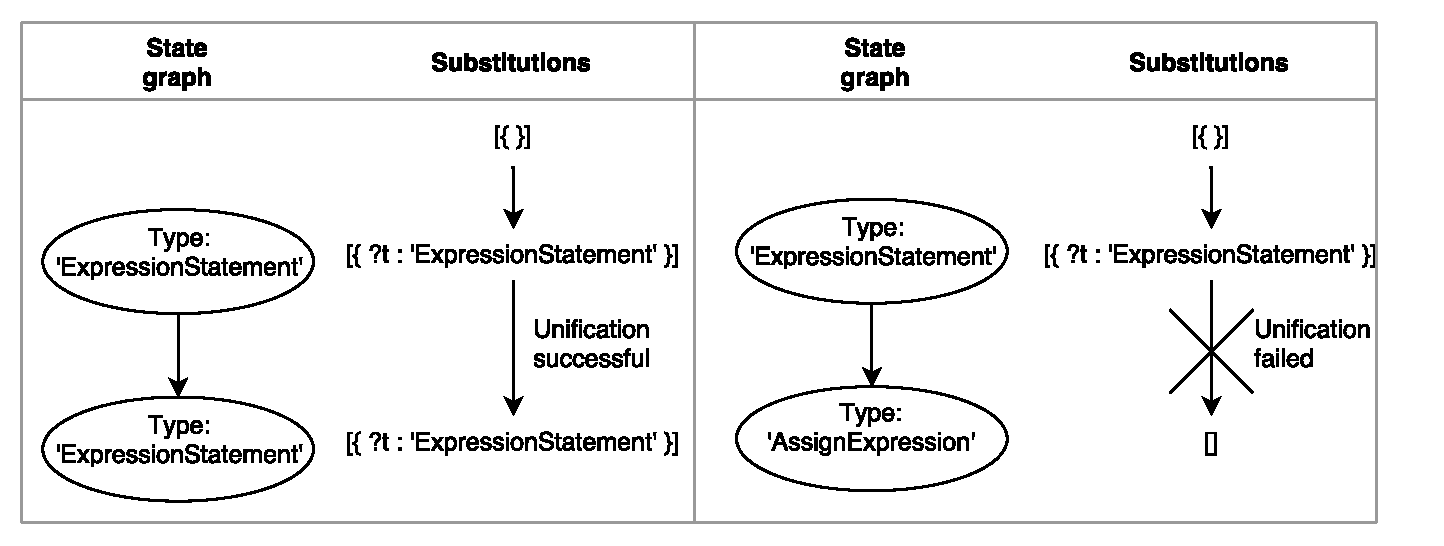
\includegraphics[width=1\textwidth]{images/Unification} 
      \caption{Visual representation of the unification process}
    \label{fig:Unification}
\end{figure}

All queries presented until now match the state graph from the beginning of the graph only. This behaviour is often undesirable as a developer usually wants to detect a pattern \textit{somewhere} in his code, not necessarily at the beginning. To resolve this, JS-QL combines techniques from regular expressions with a special built-in construct, the \textit{wildcard}.

%TODO: translate variables starting with ! to ?__TMP__

\subsubsection{Wildcard}

Wildcards are usually known as 'things of which the value can be anything', and this is no exception in JS-QL. A \texttt{wildcard} serves the sole purpose of matching any state it gets compared with. In other words, an equally correct name for this construct could have been \texttt{skip}, as it skips a state in both the query (the \texttt{wildcard} state itself) and the abstract state graph (the state the wildcard gets matched with). When talking about states in a query pattern, both \texttt{state} as \texttt{wildcard} match this definition. \texttt{wildcard}s act just like regular \texttt{state}s in a query, meaning that they only match \textit{1} state in the state graph. It is very unlikely that a developer knows exactly after how many states a violation would occur, so simply enumerating wildcards followed by the state to be matched would typically be a very tiresome effort. We therefore need to be able to specify that we wish to skip \textit{zero or more} states before matching the following state in the query pattern. This is where the power of regular expressions comes in handy. Just like regular expressions, JS-QL supports the use of both the Kleene star (\texttt{star}) and the Kleene plus (\texttt{plus}) operators. In our language, the \texttt{star} and \texttt{plus} constructs are both placed \textit{after} the state(s) they are applied to. Placing \texttt{star} behind a sequence of states indicates that those states can occur \textit{zero or more} times at the current position in the state graph. The semantics of \texttt{plus} are very similar, except for the fact that the states have to occur at least once in the order they are specified. Just like with regular expressions, pieces of a pattern can be surrounded by braces. Left and right braces in JS-QL are denoted by \texttt{lBrace} and \texttt{rBrace} respectively. The default behavior of both the kleene star and kleene plus operators is to apply them to the state that occurs right before it. If any kleene operator has to be applied to multiple states, these states have to be wrapped in braces in JS-QL. Listing \ref{lst:KleeneOperations} shows the differences. Lines 1 and 2 are semantically equivalent, as the braces on line 2 only contain 1 state, a \texttt{wildcard} in this case. Lines 3 and 4 on the other hand are semantically very different. The query on line 3 matches all but the first states in the state graph, whereas the query on line 4 matches every other state in the graph, starting from the second state. The combinations of \texttt{wildcard().star()} and \texttt{wildcard().plus()} are so commonly used in JS-QL, that a special construct is created for each of them: \texttt{skipZeroOrMore()} and \texttt{skipOneOrMore()} respectively.

\begin{lstlisting}[label={lst:KleeneOperations},language=JSQL,caption=Kleene operations differences,mathescape=true]  % float=t?

G.wildcard().star() // Equal to G.skipZeroOrMore()
G.lBrace().wildcard().rBrace().star()
G.wildcard().state().plus()
G.lBrace().wildcard().state().rBrace().plus()
\end{lstlisting}

\subsubsection{Disjunction}

Sometimes when writing a query, more than one state on the path is allowed for the query to match. Consider a simple language in which we want to detect all uses of a variable \texttt{v}. Using a variable in this language can only be done by using it in an binary arithmetic expression. To keep the example simple, we disregard all other possible uses of a variable. We also assume in this example that no other variable was assigned the value of \texttt{v}, so that no aliases of \texttt{v} exist in the code. When using a variable in a binary arithmetic expression, the variable can be on either side of the operator. A naive solution to query for all uses of \texttt{v} would be to first launch a query that finds all occurences of \texttt{v} on the left-hand side, followed by a query that detects all occurences on the right-hand side. To alleviate the work of the user, JS-QL offers the disjunction construct \texttt{or}, which allows to specify that 1 state in the state graph can be matched by multiple states in the query pattern. If we then were to match all occurrences of \texttt{v} on the left- and right-hand side of arithmetic expressions, we could write a query as in listing \ref{lst:disjunction}.

\begin{lstlisting}[label={lst:disjunction},language=JSQL,caption=The JS-QL disjunction operator,mathescape=true]  % float=t?

G.skipZeroOrMore()
.lBrace()
  //Left-hand side with name 'v'
  .state({node: { type: 'BinaryExpression',
                  left: {name:'v'}}})      
  .or()
  //Right-hand side with name 'v'
  .state({node: { type:  'BinaryExpression',
                  right: {name:'v'}}})
.rBrace()
\end{lstlisting}

This query first skips zero or more states, starting from the beginning of the graph. It then matches a \texttt{state} (\texttt{evalState} would be equally correct) with a \texttt{node} property of type 'BinaryExpression'. Remember that the node property of evaluation states contains the AST information for the current expression. Because of this, the \texttt{left} and \texttt{right} properties of the BinaryExpression are again nodes that can be further deconstructed. The \texttt{or} construct splits the query in two different query paths. One path will try to match the pattern specified before the construct, whereas the other path searches for matches for the pattern specified after the \texttt{or}. The same rules apply w.r.t. braces as for the \texttt{star} and \texttt{plus} operators. For the first path, we deconstruct the left property of the node and match its name with the literal \texttt{v}. This automatically filters out all states for which this condition doesn't hold. What remains is a match for each state for which the condition holds. The same is done for the second path, with the only difference that the name of the right node now has to be equal to \texttt{v}. As the query doesn't store any variables along the path, the result of the query can only be observed in the visual representation of the abstract state graph. In this graph, all matching nodes will be marked with color, indicating a match.

When examining the example above, we notice that very few relevant information is available as a result of the query. A more detailed result should contain the actual node or even the entire state that was matched, so we could inspect it further. To this extent, an additional implicit property was made available for each deconstructable map in the language. This property represents the entire object by which it is encapsulated. We chose to give this property an appropriate name, indicating that it points to the object currently being inspected, namely \texttt{this}. Listing \texttt{lst:updatedDisjunction} gives an updated version of the relevant code from the previous example. In this version, the \texttt{thisNode} variable will be bound to the node of the matched state.

\begin{lstlisting}[label={lst:updatedDisjunction},language=JSQL,caption=Using the \texttt{this} keyword,mathescape=true]  % float=t?

//...
.state({node: { this: '?thisNode',
                type: 'BinaryExpression',
                left: {name:'v'}}})     
//... 
\end{lstlisting}

\subsubsection{Specifying additional properties}

Sometimes it can be useful to capture extra information about already matched variables. Doing so in a separate section, exclusively designed for this purpose, has two advantages. First of all, it enhances the readability of queries. Queries with deeply nested maps can quickly become confusing to read and bothersome to modify. Secondly, it opens up for opportunities to make the language even more expressive. JS-QL has a built-in keyword \texttt{properties}, which can be used to obtain more information from already bound variables. 

Expressing properties can be done in two ways, as indicated in listing \ref{lst:propertiesExample}. As the language we are using is an embedded language, we can take advantage of the host language. JavaScript allows the value of key-value pairs to be a function call with arguments. We can we can benefit from this by defining a JavaScript function \texttt{prop}, to which we can pass which kind of information we wish to obtain and from which variable we want to obtain these properties. The first argument of \texttt{prop} is the function that needs to be applied when the matching engine processes the query. The arguments of this function are all other arguments that were passed to \texttt{prop}. Line 5 of the example below shows how to properly use the \texttt{prop} function. We have to defer the evaluation of the function passed as a first argument to \texttt{prop} because at compile-time the values of the variables aren't calculated yet (as no matching has happened). This function, in the example below 'memberOf', can be a user-specified function or a built-in function. More details on how users can specify their own functions is duscussed in section \ref{subsec:DefiningPolicies}. As for now, JS-QL only has three build-in functions that work on variables, and all three require that variable to be of type \textit{Array}:

\begin{enumerate}
\item \textit{length}: A query could contain \texttt{prop('length', '?arr')}, where \texttt{?arr} is a variable with a value of type \texttt{Array}. The function then returns the length of the array bound to the variable.
\item \textit{at}: This function takes 2 additional arguments: A variable containing an array, and an index \texttt{i}. The resulting value is the \texttt{i}th element of the array.
\item \textit{memberOf}: This function is the most important and also most used one. It takes a variable containing an array \texttt{arr} as an argument and expands the current substitution set, so that for each element in \texttt{arr} a new substitution set is created with that element appended to it. In the example below, the substitution set before the execution of line 5 would look like \\\texttt{[\{?decls : [dec1, dec2]\}]}, \\and would afterwards look like: \\\texttt{[\{?decls : [dec1, dec2], ?dec : dec1 \},\\\phantom{ }\{?decls : [dec1, dec2], ?dec : dec2 \}]}
\end{enumerate}

\noindent Another way to define properties is by simply specifying which attribute of a variable one wishes to capture. Line 6 of the example below shows how the 'name' of the 'left' attribute of \texttt{?dec} is bound to \texttt{?decName}. Declaring a new property variable is done similarly for both ways of defining properties: The key of the map should contain the variable name to be declared, whereas the value should be the property specification. One might notice that this order of key-value pairs is different from all other notations in JS-QL. This is because the host language doesn't allow function calls to be keys in maps, and thus restricts the syntax of our language in that way.

The example below matches all states of the state graph that declare variables. These declarations are captured in \texttt{?decls}. Next, for each declaration, a new substitution set is generated by the 'memberOf' function. Each substitution set now contains a variable \texttt{?dec} bound to an element of the \texttt{?decls} array. Finally, the name of the declaration in each substitution set is captured in \texttt{?decName}.

\begin{lstlisting}[label={lst:propertiesExample},language=JSQL,caption=Specifying additional properties in JS-QL,mathescape=true]  % float=t?

G.skipZeroOrMore()
.state({
      node:{ declarations: '?decls' },
      properties:{
        '?dec'     : prop('memberOf', '?decls'),  // \texttt{prop} notation
        '?decName' : '?dec.left.name'             // attributes notation
      }})
\end{lstlisting}

It is very important to keep in mind that only the variables that are already bound can be used in properties. This implies that the order of the keywords in a query is important for the semantics of the query. If we were to switch the \texttt{node} and \texttt{properties} keywords of the above query, an error would occur because the \texttt{?decls} variable wouldn't be available to use in the properties section.

\subsubsection{Filtering states}

Filters in JS-QL work very similar to properties, except that they act as guards who filter out states that don't satisfy certain conditions. A filter can be any function, predefined or specified by the user, that returns a boolean value. When returning true the pattern can be matched further, otherwise the matching process aborts and no match for the current path in the state graph is found. A filter is declared through the \texttt{cond} JavaScript function (similar to \texttt{prop} for filters), and takes a filter function as a first argument. All other arguments are passed as the arguments to the filter function. As no variables have to be stored for filters, the notation is not traditional in such a way that it doesn't use map. Instead, a JavaScript array lists all filters to be satisfied. Consider the following example: JavaScript allows the declaration of multiple variables in one declaration statement, e.g.:\\\texttt{var a = 1, b = 2;} \\Some companies see this as a bad practice, as it is harder to maintain and less error-prone. A query can be written to to detect all violations of this company policy, by storing the length of the declarations in a variable and checking if the length of the variable is larger than 1. Only the states for which this filter is satisfied will be contained in the results of the query. Listing \ref{lst:multipleDeclarations} illustrates this example.

\begin{lstlisting}[label={lst:multipleDeclarations},language=JSQL, caption=Filtering for multiple declarations,mathescape=true]
G.skipZeroOrMore()
.state({
      node:{declarations: '?decls'},
      properties:{
        '?length' : prop('length', '?decls')
      },
      filters:[
          cond('>', '?length', 1)
      ]
    }) 
\end{lstlisting}

\subsubsection{Data flow in JS-QL}

Support for data flow opens up to write a whole new class of queries. As JavaScript is a dynamic language, any variable can be assigned to any other variable. This phenomenon is known as \textit{aliasing}, and is very common in the language. As already discussed in chapter \ref{ch:Overview}, JIPDA stores the addresses and values of variables in the \texttt{store}. Values stored for primitive types are indistinguishable in the store, because of abstract interpretation:\\
\texttt{var x = 4; var y = 9999;}\\
Both x and y are integers and will point in the store to a value of \texttt{\{Num\}}. We thus can't track aliasing for primitives. Reference types in JavaScript however are distinguishable in the store as they each point to a set of unique addresses for that reference. Remember that reference types can point to multiple addresses as a consequence of precision loss of abstract interpretation. A feature of the abstract state graph that affects the expressiveness of our language is that it displays states as they are evaluated. This means that for assignments for example, the address of the left-hand side of the assignment often isn't available in the assignment state, as the value (and address) of the right-hand side needs to be evaluated first. This happens \textit{after} the assignment state in the state graph. An example is the simple program: 
\texttt{var x,y; x = \{\}; y = x;}
In this program, \texttt{x} gets assigned a fresh object, after which it gets aliased to \texttt{y}. \texttt{x} and \texttt{y} point to the same set of addresses after execution of this part of the program.
The relevant graph part is depicted in figure \ref{fig:AssignmentLookup}

\begin{figure}[!h]
    \centering
      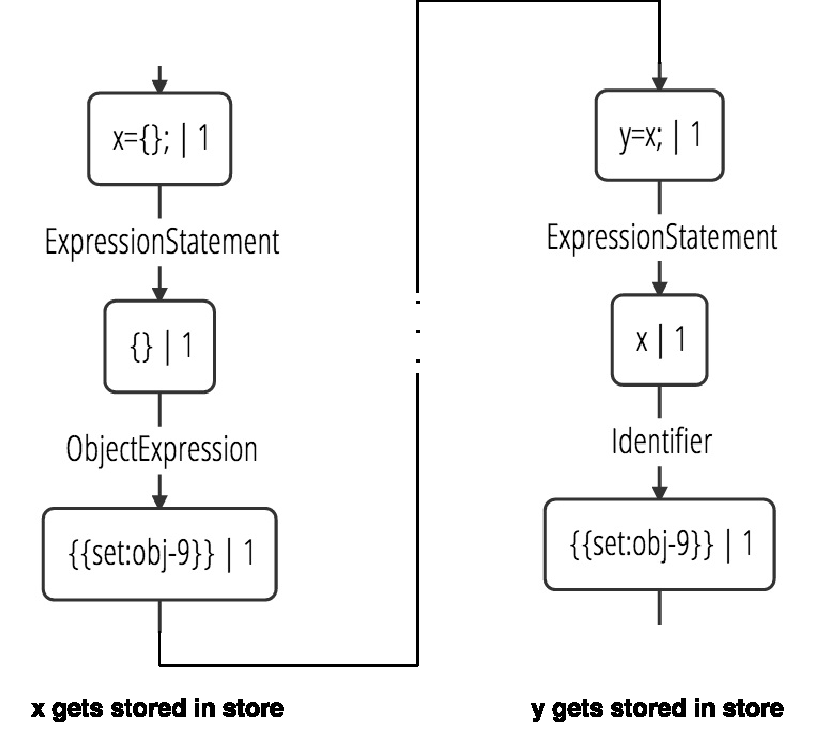
\includegraphics[width=.5\textwidth]{images/assignmentLookup} 
      \caption{Assignment representation in the state graph}
    \label{fig:AssignmentLookup}
\end{figure}

The problem with this kind of representation in the graph is that when we try to match the assignment in a query, no address information for \texttt{x} is available. After evaluating the fresh object, \texttt{x} gets stored in the store. Later on in the program, \texttt{y} gets assigned the value of \texttt{x}. Now, there is no problem because the address of \texttt{x} is already available in the store, so it can be looked up in the query. Note that the data flow detection in JS-QL isn't nearly as powerful as for example a taint analysis. Queryies and policies can be written to mimic a taint-analysis, but this requires some work. Later in this chapter we will discuss how custom queries and policies can be defined.

Variables can be looked up in JS-QL using the \texttt{lookup} keyword. The value-part of this keyword is again a map with the names of the variables to lookup as keys, and the variable names that need to be bound to the addresses as values. Performing a lookup in JS-QL happens by first looking into the lexical scope. When variables with the same name are defined in both a function and the global scope, the lookup value of that variable will depend on the state that is currently matched. Therefore, we need to provide some sort of mechanism to 'overwrite' this default behavior, in case the address of the global variable is needed when the currently matched state is inside a function application. To this extent, JS-QL recognizes the \texttt{\_global} string as an indicator to perform a lookup in the global scope. Listing \ref{lst:lookup} shows how variables can be looked up. First, the name of the right-hand side node of the assignment expression gets bound to \texttt{?rn}. When the assigment expression gets matched with a state in the global scope, all three address variables \texttt{?rnAddr}, \texttt{?globrnAddr} and \texttt{?xAddr} will have the same value. However, when the assignment on line 7 gets matched, \texttt{?globrnAddr} will point to the globally defined \texttt{x}, whereas the other two lookups contain the address of the locally defined \texttt{x}.

\begin{lstlisting}[label={lst:lookup},language=JSQL, caption=Looking up addresses in JS-QL,mathescape=true]
//Javascript program
var x, y;
x = {};
y = x;
var f = function(){
  var x = 4; //local x gets declared
  y = x;
}
f();
//JS-QL query
G.skipZeroOrMore()
.state({node:{
          expression:{
            type:'AssignmentExpression', right: {name:'?rn'}
        }},
        lookup:{
          '?rn'        : '?rnAddr',     //lookup by variablename
          '_global.?rn': '?globrnAddr', //lookup in global scope
          'x'          : '?xAddr'       //lookup based on name
        }})
\end{lstlisting}



\subsubsection{Negation}

Expressing which statements and expressions we want to detect on a path in the graph is made easy by JS-QL. Sometimes however, this doesn't suffice for some queries. In some languages, accessing a file after it was closed results in an error in the application. This might compromise the integrity of the system. A naive approach to writing a policy for this would be to detect all calls to the \texttt{access} method that follow, after some wildcard states, the call of a \texttt{close} method for a file \texttt{f}. While this query would match and return all violations against the policy, false positives would occur. This is because of the wildcard states between the two function calls. One of these calls could be a call to the \texttt{open} method, meaning that accessing the file afterwards is permitted.  A better approach would be to specify that we \textit{don't} want to encounter a call to \texttt{open} for \texttt{f} between closing and accessing it. This is exactly what the \texttt{not} construct does. When placing this construct right before a state, the query will only be matched if the negated state can't be matched with the current state in the state graph. When placing \texttt{not} before a state, and \texttt{star} or \texttt{plus} right after that state, it can be read as: "Match zero/one or more states that are \textit{not} the negated state". A better query for the example above would then be written as in listing \ref{lst:OpenClosedFile}, which can be found in the appendix for brevity reasons. The query first skips several states until it reaches a call to \texttt{close} on file \texttt{f}. The address of the file to be closed is also stored in a variable to correctly detect only the accessing and opening of that specific file. Next, all states are matched that are not opening \texttt{f}. Finally, the actual violation is detected, namely accessing the file after it has been closed and not re-opened. Negation is in the current version of JS-QL subject to some limitations: 
\begin{enumerate}
\item Variables that are bound in a negated state, are only visible to that state. They will thus not be included in the resulting substitutions.
\item Currently, only one state can be negated. Negating sequences of states wrapped in braces is not yet supported.
\end{enumerate}

%\subsubsection{Summary of constructs}

%SUMMARY OF BUILT-IN CONSTRUCTS

\subsection{Types of queries}
\label{subsec:TypesOfQueries}

The most straightforward way to query for properties is by just specifying a pattern and an input program. The pattern is then checked and each violating path is reported in the results. Sometimes however other types of queries are needed for the detection of specific policy violations. In this section we discuss the different types of queries and how they can be used.

\subsubsection{Existential queries}
All queries already presented in this chapter are existential queries. They report a violation of a policy for each path on which they encounter the violation. Existential queries can be defined as follows:
\begin{definition}
\textbf{Existential queries}: Given an edge-labeled directed graph $G$ where labels may have parameters, a vertex $v0$ in $G$, and a parametric regular-expression pattern $P$, compute all pairs of vertex $v$ in $G$ and a substitution $\theta$ for parameters in $P$ such that there exists a path from $v0$ to $v$ in $G$ that matches some sentence accepted by $P$ under $\theta$.
\end{definition}

\noindent What this means is that \textit{any} path in the state graph matching user-defined query will produce a resulting substitution. For that path, the policy has been violated, but chances are that that path never gets executed when actually running the program, as a consequence of the overapproximations of the static analysis in JIPDA. A branch of a conditional might never be executed in a program for example. If the value of the test in the conditional gets overapproximated (i.e. with an abstract value of \textit{\{Bool\}}), the state graph will depict both branches, as it can't decide which branch will be taken. Existential queries thus match a pattern \textit{if there exists a path} in the state graph matching the query.

\subsubsection{Universal queries}

Sometimes detecting if a pattern occurs along a path in the state graph doesn't suffice. Universal queries provide stronger guarantees for queries, as they require that the query matches for the same substitutions along all possible paths in the state graph between two states. We define universal queries as follows:
\begin{definition}
\textbf{Universal queries}: Given an edge-labeled directed graph $G$ where labels may have parameters, a vertex $v0$ in $G$, and a parametric regular-expression pattern $P$, compute all pairs of vertex $v$ in $G$ and substitution $\theta$ for parameters in $P$ such that every path from $v0$ to $v$ in $G$ matches some sentence accepted by $P$ under $\theta$.
\end{definition}

The intrinsic difference between universal and existential queries is how they match a pattern. Where it suffices for existential queries that just one path exists in the state graph, universal queries make sure that \textit{all} paths between two points in the graph match the specified query. For the sake of a representative example, imagine a JS-QL predicate \texttt{def(\{name:'?x'\})}, which checks all definitions and redefinitions of a variable bound to \texttt{?x}. This variable has a constant value in the state graph as long as no redefinitions of \texttt{?x} happens along any path between two states in the graph. We can then query for each state in the graph where \texttt{?x} has a constant value. The query in listing \ref{lst:UniversalQuery} shows how this can be expressed in JS-QL. Creating such predicates will be discussed in the next section. The definition of a variable \texttt{v} is matched, and any state following that matched state that isn't a redefinition of \texttt{v} will be contained in the result. All states in the state graph up until a redefinition of \texttt{v} (or the end of the graph) will then be marked in color in the user interface.

\begin{lstlisting}[label={lst:UniversalQuery},language=JSQL, caption=Checking for constant folding using a universal query,mathescape=true]
G.skipZeroOrMore()
.def({name: '?x'})            // Define the variable
.not().def({name: '?x'}).star // As long as it isn't redefined
\end{lstlisting}

\subsubsection{Query direction}

Queries in most traditional systems are viewed as straightforward, in the sense that they match a part of a graph or other program representation from point $a$ to $b$. This way of reasoning implies that queries are always matched from the beginning to the end of a program (if control-flow information is available, that is). Our framework supports this manner of querying in the traditional way, but also allows to explore the state graph bottom-up. This can be meaningful to search for certain program properties. \textit{Forward} queries are queries as we've defined them until now. They match the state graph from the beginning state to the resultstates and are pretty easy to understand and read. \textit{Backward} queries on the other hand traverse the graph in a bottom-up manner, meaning that the query starts at the end of the state graph and matches states until the starting state of the graph is reached. Although backward queries are less common they can be useful to perform some program analysis, such as live variables analysis. This analysis calculates for each program point the variables that may be potentially read before their next write. A variable is thus live if it holds a value that may be needed in the future. The backward query for this analysis goes as follows:

\begin{lstlisting}[label={lst:Liveness},language=JSQL, caption=Live variables anlysis in JS-QL,mathescape=true]
G.skipZeroOrMore()
.use({name: '?x'})            // Read the variable 
.not().def({name: '?x'}).star // As long as it isn't written
\end{lstlisting}

The \texttt{use} and \texttt{def} predicates are again user-defined predicates. Starting from the resultstate of the program, some states are skipped until the first use of variable \texttt{?x} is found. Note that this is in fact the \textit{last} use of that variable in the state graph for that liveness set. The query then marks all states that aren't a write to \texttt{?x}. In this way, one or more states will be marked, representing the path on which variable \texttt{?x} was live.

\subsection{Defining predicates and policies}
\label{subsec:DefiningPolicies}

Expressing queries and policies with only the \texttt{state} and \texttt{wildcard} constructs quickly becomes tiresome as every attribute of the state has to be explicitly specified. The JS-QL framework remedies this by letting users specify their own predicates and policies as well as by providing some basic customizable predicates for single expressions and statements.
We can distinguish predicates and policies by what they match. Predicates are like the \texttt{state} construct, in the sense that they match only one specific state. For example, JS-QL has a built-in predicate \texttt{functionCall} which matches function calls. The nice thing about these predicates is that a user can specify what he wants to match in a state. Policies on the other hand are sequences of predicates and/or \texttt{state}s, forming a pattern. We will demonstrate how to write predicates by dissecting a relatively simple built-in predicate called \texttt{assign}. All predicates and policies can be written in a separate file, as long as they are extend in the \textit{JSQL prototype}:\\
\texttt{JSQL.prototype.assign = function(obj)\{\ldots \}}\\
This is the basic notation for named predicates, in this case the \texttt{assign} predicate. The dots in the code above will be filled in by the actual predicate code. We immidiately notice the \texttt{obj} argument. This argument represents the map of all properties of the state that need to be matched. By abstracting the map to a single \texttt{obj} variable, the user is free in which properties and attributes he wishes to match or omit for a specific query. The usefulness of predicates would drastically be reduced if the user has to again pass a nested map of properties to the predicate. We therefore let the developer of the predicate decide which properties he wishes to match, and how he names these properties in the predicate. For the example of the \texttt{assign} predicate, we chose to provide 3 basic attributes to the user: \texttt{this}, \texttt{left} and \texttt{right}, representing the whole assignment node, its left- and right-hand side resp.
\begin{lstlisting}[label={lst:predicateArguments},language=JavaScript, caption=State properties of the \texttt{assign} predicate,mathescape=true]
var s = {}; // variable representing the state
var objThis  = this.getTmpIfUndefined(obj.this); 
var objLeft  = this.getTmpIfUndefined(obj.left); 
var objRight = this.getTmpIfUndefined(obj.right); 
\end{lstlisting}
\noindent A particularly handy feature of JavaScript is the named keys of a map. When accessing such a key in the map (like \texttt{obj.left} for example), the corresponding value is returned when found. When no such key exists, JavaScript returns \texttt{undefined}. To ease the use of predicates, some attributes in the \texttt{obj} map can be made optional. We do this by using the \texttt{getTmpIfUndefined} method, which returns a \textit{temporary variable} when the value for its argument is \texttt{undefined}, and the regular value (a literal or a variable) when it is contained in the map. Temporary variables are variables that won't be contained in the resulting substitutions. By introducing these variables in the code, no conditionals have to be written that check whether an attribute has been specified in the map of a predicate, as we can then just use the temporary variable as a replacement. We instantiate a variable for each attribute as seen in the example. Remember that the attributes can have any name as long as it is clear to the user what the attribute stands for: \texttt{obj.right} could have also been \texttt{obj.abc}, but that would harm the readability of the predicate and confuse the user.

Mapping the attributes of the \texttt{obj} map to a state happens by setting up the state chain. To make things not too complicated for query and predicate developers, we provide a \texttt{setupStateChain} method which does just that. As can be seen in the example above, a map that mimics a state of the state graph is defined though variable \texttt{s}. This variable will be used to build the mimicked state. For each attribute that we provide through the predicate, an entry has to be made in the state map \texttt{s}. We indicate which piece of information we want to match by passing an array of keys we want to traverse in a state as a second argument to \texttt{setupStateChain}. The last key of this array will have the third argument as its value. The first argument is the map in which we want to store this information. When executing line 1 and 2 of listing \ref{lst:predicateState}, \texttt{s} will now contain 1 direct attribute \texttt{node}, which will in turn have 1 attribute \texttt{expression}, which will finally have 2 attributes, \texttt{left} and \texttt{right}. As we only match assignments, we filter the operator of the expression to be '=' on line 4. Note that this is not limited to querying the \texttt{node} property of a state. All information in the state graph can be queried through a predicate.
\begin{lstlisting}[label={lst:predicateState},language=JavaScript, caption=State chain setup of the \texttt{assign} predicate,mathescape=true]
this.setupStateChain(s,['node','this'], objThis);
this.setupStateChain(s,['node','expression','left'], objLeft);
this.setupStateChain(s,['node','expression','right'], objRight); 
this.setupStateChain(s,['node','expression','operator'], '='');
\end{lstlisting}

We want to be able to specify properties, filters and lookups as in regular states. JS-QL allows this in the same way as in states. Putting everything together happens by finalizing each state map (only \texttt{s} in this case) and specifying the state(s) that match the predicate/policy. Listing \ref{lst:predicateFinalize} shows how finalization is done and how the pattern is specified. Finalizing handles things like lookups, filters and properties through the \texttt{finalize} method. This method extracts all relevant information from the \texttt{obj} map and adds it to the state map it gets as a first argument. Finally, the pattern is specified and each state in the pattern gets initialized its own designated state map. For predicates, there will always be at most one state map. Policies however can have multiple state maps, as they represent a sequence of states, each with their own map. This is the only characteristic in which predicates and policies differ. An example of a policy can be seen in listing \ref{lst:WriteToBuiltinObjectPrototype} in the appendix.

\begin{lstlisting}[label={lst:predicateFinalize},language=JavaScript, caption=Finalizing the \texttt{assign} predicate,mathescape=true]
this.finalize(s, obj); //Finalize a specific state
return this.state(s);  //Fill in the state map
\end{lstlisting}

The full code for the predicate is listed in \ref{lst:assignPredicate} in the appendix. We can now use this predicate in any query, with the arguments that we wish to match in a state, as seen below:

\begin{lstlisting}[label={lst:assignCall},language=JSQL, caption=Using the \texttt{assign} predicate,mathescape=true]
G.skipZeroOrMore().assign({left: '?l'})
G.skipZeroOrMore().assign({right: '?r'})
G.skipZeroOrMore().assign({left: '?l', right:'?r',
                           properties:{
                              '?rName' : '?r.name'
                           },
                           lookup:{
                              '?rName' : '?rAddr'
                           }}) 
//And so on ...
\end{lstlisting}

\subsubsection{recursion}
%moet dit naar types of queries?
Some types of queries or analyses require that a variable is reintroduced in several consecutive states, or that a trace of information is kept along each state. This behavior can be achieved by defining \textit{recursive queries}. Recursive queries are queries that can invoke themselves again, until a base case is matched. This type of query can for example be used to detect by which variables a variable is tainted (i.e. influenced/marked). JS-QL supports recursive queries by providing the \texttt{rec} function. This function takes two arguments: (i) The mapping for the next recursive step and (ii) the predicate/policy that needs to be called recursively. The \texttt{taintedBy} policy is included in the appendix as listing \ref{lst:taintedBy}. It describes a naive taint analysis which only considers simple assignments. It takes three arguments, which can all be omitted: \texttt{orig} denotes the original value which will be aliased, \texttt{alias} represents the alias of the original value and \texttt{rec} keeps track of all variables that have been used as aliases inbetween \texttt{orig} and \texttt{alias}. The relevant code of the policy is found below:

\begin{lstlisting}[label={lst:recursivePolicy},language=JSQL, caption=Recursive call of the \texttt{taintedBy} policy,mathescape=true]
this.setupStateChain(s1, //State map s1
                    ['node','expression','right','name'], orig); 
this.setupStateChain(s1, //State map s1
                    ['node','expression','left','name'], alias); 
this.setupStateChain(s2, //State map s2
                    ['node','expression','right','name'], orig);
this.setupStateChain(s2, //State map s2
                    ['node','expression','left','name'], flow);

return this .lBrace()
            .state(s1)                  //1. From orig to alias
            .or()
            .state(s2)                  //2. From orig to flow
            .skipZeroOrMore()           //   Skip some states
            .rec(newObj,this.taintedBy) //   From flow to alias
            .rBrace();

//JS-QL query:
G.skipZeroOrMore({orig: '?o', alias:'?alias', rec:'?r'})
\end{lstlisting}

The policy matches all simple assignments by name. Lines 1-8 set up the state maps of 2 separate states. The first state matches a direct assignment from \texttt{orig} to \texttt{alias}. The second state does the same, but the alias in this case is an intermediate assigned variable \texttt{flow}. So when we assign $a$ to $b$ and $b$ to $c$, the resulting state can look like: \{orig: a, flow: b, alias: c\}, indicating that $c$ is an alias of $a$, and that it obtained the value of $a$ through $b$. Lines 10-16 show the pattern that needs to be matched. Or we match an assignment directly (the base case), or we match a state from \texttt{orig} to \texttt{flow}, and later in the graph from \texttt{flow} to \texttt{alias}. The recursive call will keep occuring until no more match is found in the state graph, or when the base case is matched. This policy clearly shows that recursive queries can also be used to discover data flow properties of a program. When writing a policy similar to \texttt{taintedBy} which also keeps track of the address of the values, even more accurate data flow properties can be detected.

\subsection{conclusion}
In this chapter we described the syntax and usage of the JS-QL language. We discussed the basic constructs used to build queries in section \ref{subsec:Syntax}, as well as more advanced predicates that are either built-in or that can be user-specified. JS-QL supports several types of policies, and each of them is described in section \ref{subsec:TypesOfQueries}.
Writing predicates and policies might seem tiresome at first glance, but actually is quite repetitive and easy to do. The benefit of predicates and policies is that they are 'write once, use often'. A method for defining custom predicates and policies is described in section \ref{subsec:DefiningPolicies}. We can conclude that the JS-QL can be learned with little effort, after which expressive queries can be written to check all kinds of code characteristics. 
 
\chapter{Implementation}
\label{ch:Implementation}
This chapter describes the implementation of the JS-QL tool and language, presented in chapter \ref{ch:JSQL}. The implementation of JS-QL is publicly available\footnote{https://github.com/voluminat0/Jipda-Security} and can be used freely to test source code for general characteristics and security vulnerabilities.


\section{Architecture}
The architecture of the implementation  separates each component in a different module, providing the possibility to replace these modules by alternative implementations. In this section we discuss what each component represents.

\subsection*{Datastructures}
The \texttt{DataStructures} module defines all datastructures used in JS-QL. These include all kinds of tuples used for the matching algorithm of our tool, but also the alternative representations of edges and nodes to transform the abstract state graph into a compatible graph for the matching engine.

\subsection*{AbstractQuery}
The \texttt{AbstractQuery} module defines the core of the matching engine. It contains all operations on substitution sets: matching, merging, defining extra properties, filters and lookups. The module provides an interface to the query algorithms \texttt{ExistentialQuery} and \texttt{UniversalQuery} (see section \ref{sec:TypesOfQueries}), which perform the actual query matching processes.

\subsection*{Automaton}
The \texttt{Automaton} module defines the uniform representation of finite state machines (also known as finite automatons). It abstracts away whether the automaton is deterministic or non-deterministic, and provides information about the accepting, starting and intermediary states of these automatons.

\subsubsection*{ThompsonConstruction}
The \texttt{ThompsonConstruction} module defines an algorithm to convert a regular expression to a NFA (non-deterministic finite automaton). It parses the regular path expression and adds required states to the newly created automaton for each step in the parsing process.

\subsubsection*{SubsetConstruction}
The \texttt{SubsetConstruction} module defines an algorithm to convert a NFA to a DFA (deterministic finite automaton). It eliminates all $\epsilon$-transitions, which are transitions that can occur without reading an input symbol. The resulting automaton is used by both query algorithms.

\subsection*{JipdaInfo}
The \texttt{JipdaInfo} module transforms state information to a more readable format for users. This transformation is necessary to enforce consistent datastructures for states containing information about an AST node. The transformed states are the actual states that are queried instead of the original JIPDA states.

\subsection*{JSQL}
The \texttt{JSQL} module defines the internals of the JS-QL query language. It is implemented as an embedded DSL in JavaScript and allows users to define application-specific predicates and policies. The module is made available for the user through a fluent interface, increasing the readability of the language.

\subsection*{SecurityAnalysis}
The \texttt{SecurityAnalysis} module glues together every component in the tool. This module invokest he initialization and transformation of the abstract state graph, as well as the execution of queries and the processing of query results.

\section{User interface}
The JIPDA analysis comes with an interface which enables the user to inspect the abstract state graph. This state graph is generated by performing abstract interpretation, provided that the user provides an input program and a lattice. For our tool we augmented this user interface in several ways described in this section. Figure \ref{fig:UI} shows the user interface. A user can specify a JavaScript program and JS-QL query in the left column of the user interface. The middle column of the interface shows the actual state graph, together with a textual representation of the results. Finally, the right column gives a more detailed report of the query results. These results can be inspected by the user, as they are represented as JavaScript objects.

\begin{figure}[h]
    \centering
      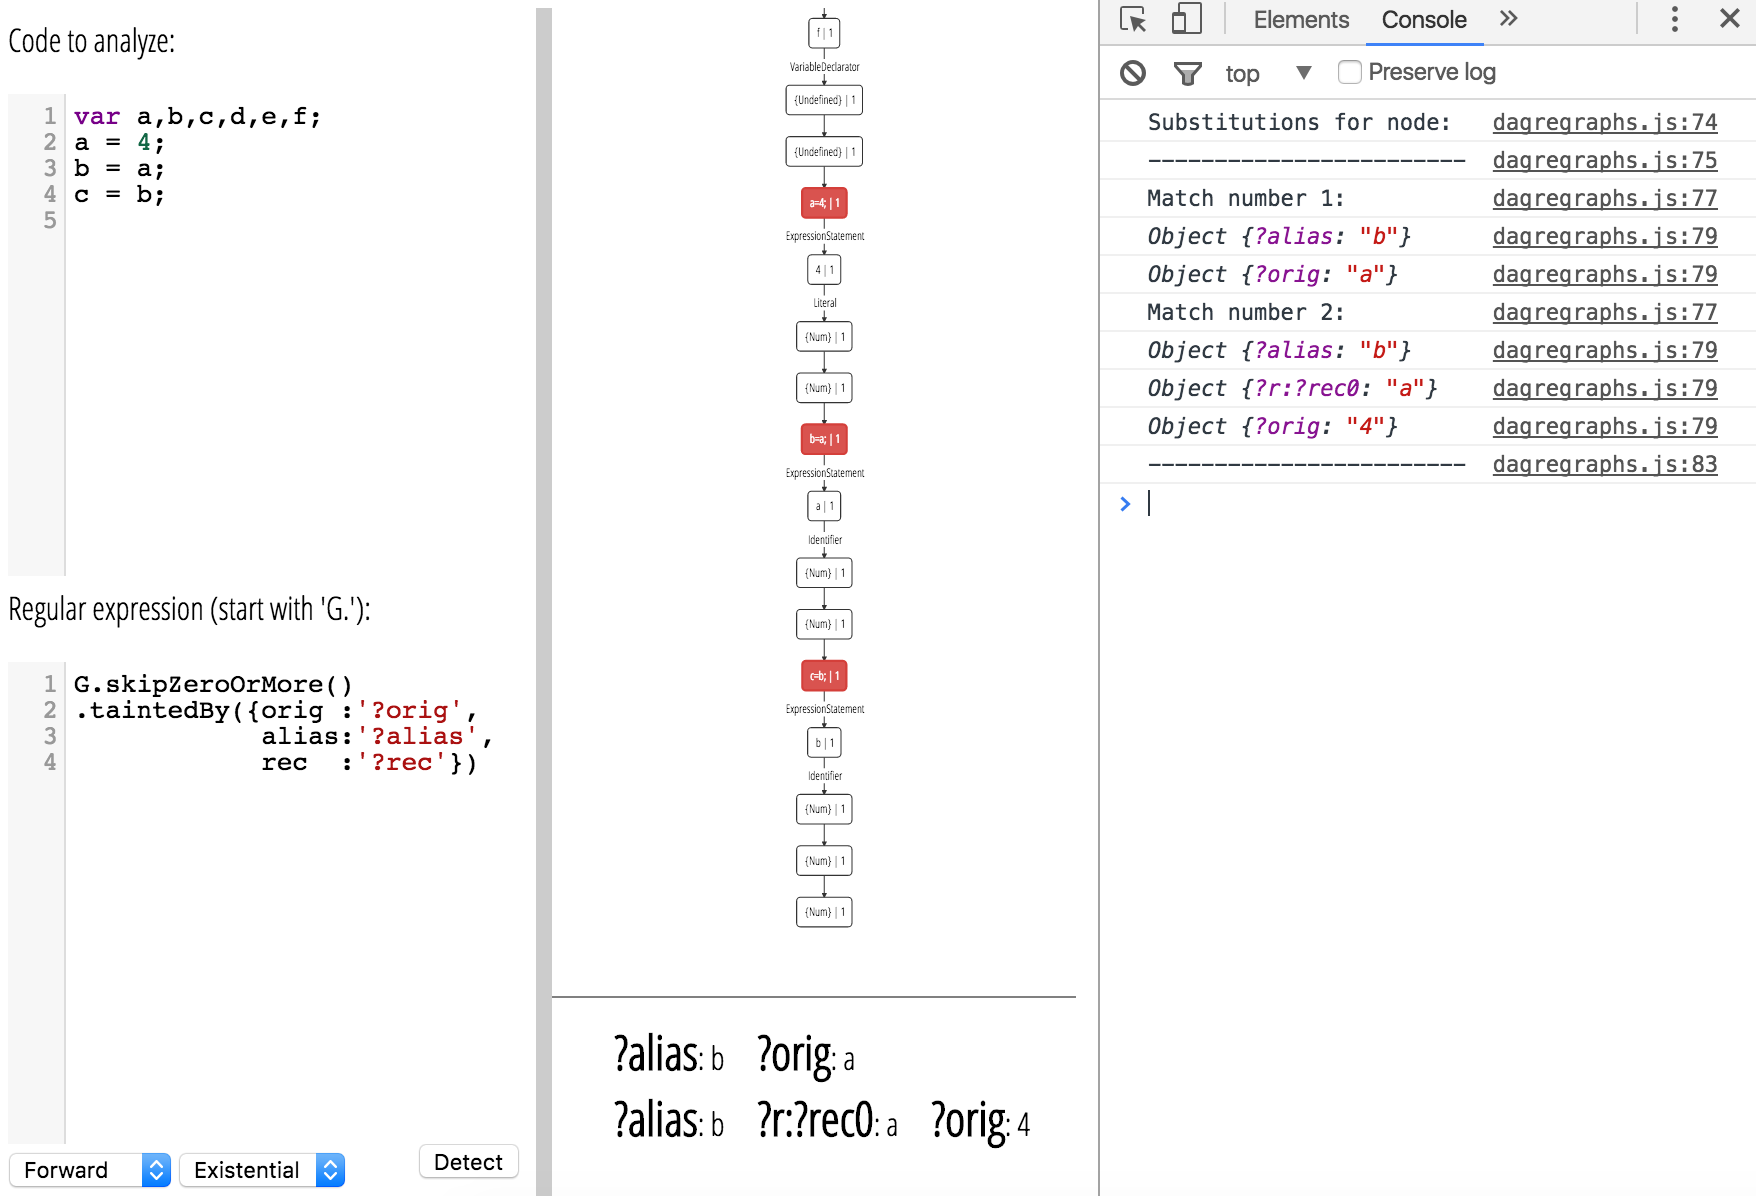
\includegraphics[width=1\textwidth]{images/UI} 
      \caption{The JS-QL tool user interface}
    \label{fig:UI}
\end{figure}

\subsection*{Query interpretation}

Our tool enables the user to specify queries in the user interface itself. This way we avoid to switch between different screens and/or files to run just one query. The user interface contains a third-party JavaScript plugin which enables syntax highlighting. The plugin is used for the input textboxes for a query and the input program. Along with entering the needed information, a user can decide the kind of query that needs to be executed. This can be done by selecting the direction (forward or backward) together with type of query (existential or universal). When pressing the 'detect' button, internally a new \texttt{Query} object is made with the provided query string. Query objects contain three fields: The query direction, its type and a \texttt{JSQL} object, representing the instantiated query. The query string is then converted to a JSQL object by \texttt{eval}uating it.

\subsection*{Abstract state graph}

JIPDA already provides the functionality to display the abstract state graph in the user interface. We modified the representation of the graph so that it became optimal for the user to reason about query results:
\begin{enumerate}
\item \textit{Edge labels}: As our approach uses edge labels to match states, we shifted information from nodes to edges. The JIPDA state graph already contains edge labels, but the information they contain is irrelevant for our approach. All evaluation states' outgoing edges are also augmented with a visible edge label representing the type of AST node it contains, to make it easier for the user to determine what to specify in his queries.
\item \textit{State colours}: The default colours of all JIPDA states have been stripped from the graph. This was done to increase the contrast with marked states (i.e. states indicating a match of the query). When the matching engine produces all results, these results are transferred to the corresponding states of the state graph. A 'marker' property was added to each matched state, containing the match information as well as a CSS class to highlight them in the otherwise colourless graph. This CSS class can be customised by the user.
\end{enumerate}

\subsection*{Results inspection}

A query result is a set of substitutions, mapping variables (denoted by a starting \texttt{?}) to their corresponding values in the state graph. Every matching state is marked with its substitution set(s). These results can then be further explored in the results section under the state graph or in the browser's built-in console, which allows inspection of results in even greater detail.


\section{The query language}
\label{sec:queryLanguageImpl}
The JS-QL query language is implemented as an embedded DSL with JavaScript as its host language. We motivated the use of a DSL in chapter \ref{ch:Overview} and explored the JS-QL syntax and semantics in chapter \ref{ch:JSQL}. This section describes how the DSL is implemented and how we incorporate several DSL implementation techniques. An overview of how queries are processed is depicted in figure \ref{fig:QueryProcessing}.

\begin{figure}[!h]
    \centering
      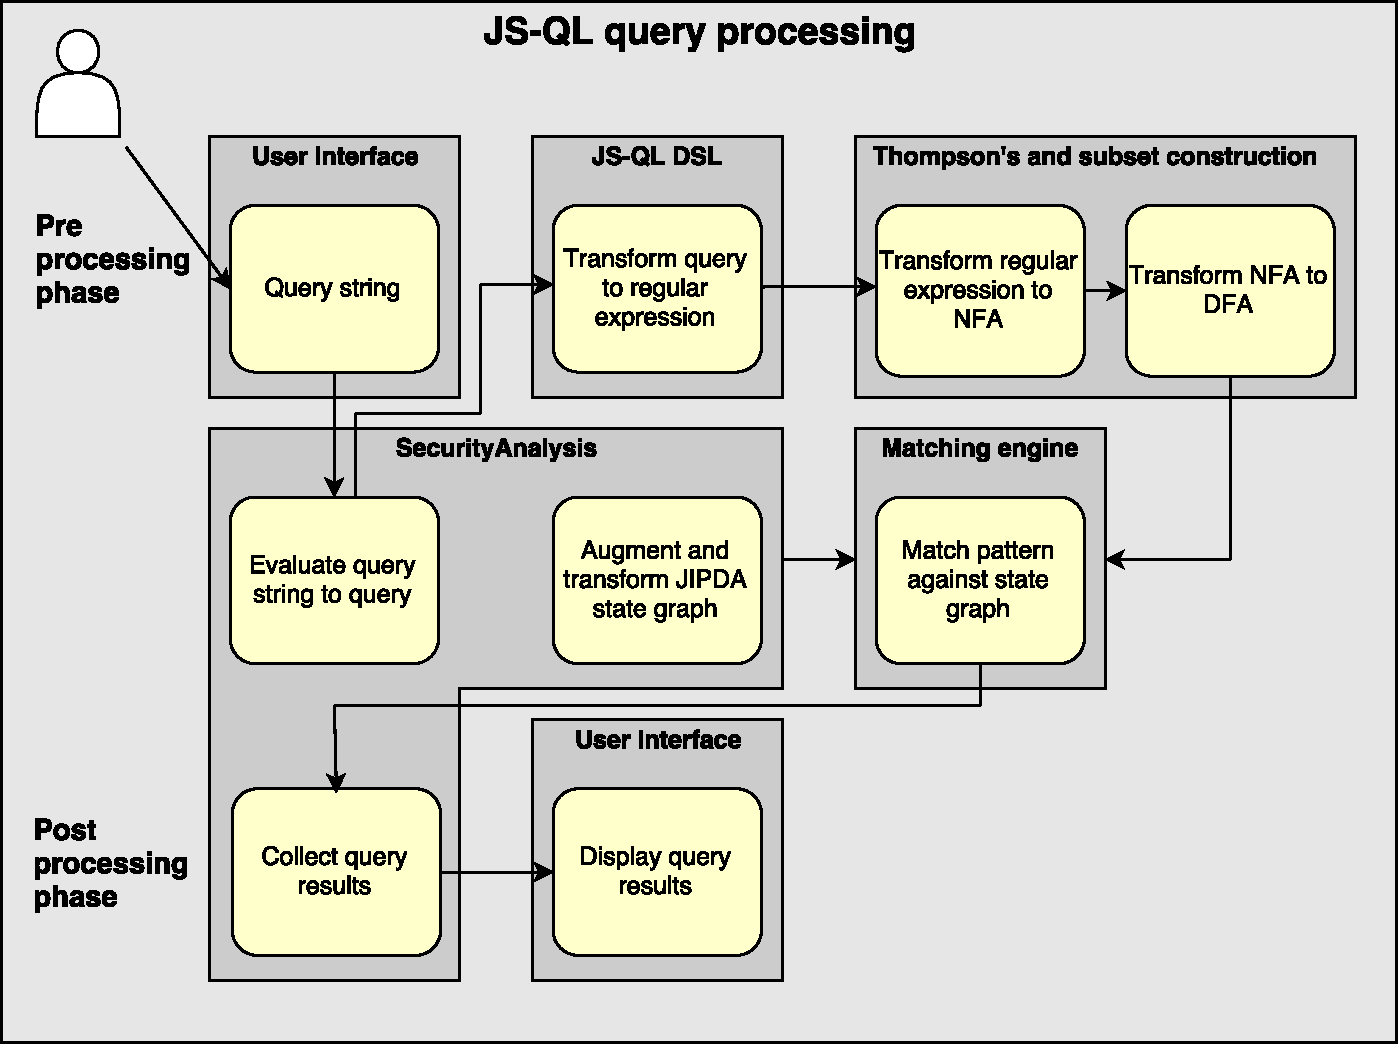
\includegraphics[width=1\textwidth]{images/QueryProcessing} 
      \caption{Stages of processing a query}
    \label{fig:QueryProcessing}
\end{figure}

\subsection*{Internal representation of pattern states}

A JS-QL query is parsed like a regular expression. Each state in the pattern represents one character in the regular expression, defined by objects of type \texttt{RegexPart}. These parts of the pattern have 5 fields to ease the translation from regular expression to automaton:
\begin{enumerate}
\item \textit{Name}: The name of a regular expression part. In the current implementation, the name denotes the type of the state/predicate that the \texttt{RegexPart} represents (e.g. \texttt{state, wildcard, not, lbrace, \ldots})
\item \textit{Symbol}: The actual symbol that will be parsed by the parser to set up the automaton corresponding to the query.
\item \textit{Object}: The argument of the state/predicate in which all variables are bound and properties, filters and lookups are specified.
\item \textit{ExpandFunction}: A higher-order function representing a recursive predicate or policy that is called for recursive queries. This argument does not need to be specified when a query is not recursive.
\item \textit{ExpandContext}: A unique identifier to avoid overlapping recursive variable names. Only used for recursive queries.
\end{enumerate}

States and predicates are function calls returning \texttt{this} to enable method chaining (which is a commonly used technique to implement a fluent interface). Each function call represents one state in the pattern, and thus for each of these calls the corresponding \texttt{RegexPart} gets pushed into a map containing the pattern information. 

\subsection*{Handling recusion}

 Recursive query patterns can contain an arbitrary number of states, so they cannot be modelled directly as a sequence of \texttt{RegexPart}s as the length of the actually matched pattern is not known. We therefore store a whole recursive query in just one \texttt{RegexPart} object, and mark it with 'subgraph' as its name. Additionally, we specify the \texttt{ExpandFunction} and \texttt{-Context} to be able to process the subgraph in the matching algorithm. The idea to treat recursive queries like this was adopted from the PQL language~\cite{PQL}. 

\subsection*{Transforming a query to an automaton}

The entire query pattern (i.e. the map) is processed by applying \textit{Thompson's Construction Algorithm} and the \textit{Subset Construction Algorithm} consecutively to obtain a NFA and DFA respectively~\cite{Thompson}. These algorithms won't be discussed in too much detail, as they are well described in many online resources and in the literature. 

\subsection*{Regular, temporary and recursive variables}

JS-QL supports three types of variables: Regular, temporary and recursive variables. Each of these types of variables play a particular role in the tool:
\begin{enumerate}
\item \textit{Regular variables} contain the information that the user wants to match in a query. When a match succeeds, they are contained in the resulting substitutions.
\item \textit{Recursive variables} are used as intermediary variables. They function as a variable that was bound in the previous step of a recursive query, enabling a recursive step to work with the value of one or more variables of the previous step. The \texttt{taintedBy} example from chapter \ref{ch:JSQL} uses a recursive variable to store all intermediary assignments.
\item \textit{Temporary variables} are state-local variables used when a user does not specify a certain argument for a predicate or policy. When only specifying the \texttt{left} argument for the \texttt{assign} predicate (See the example in chapter \ref{ch:JSQL}), the \texttt{right} and \texttt{this} attributes will be bound to temporary variables. These variables are dropped from the resulting substitutions.
\end{enumerate}

\noindent By allowing the user to choose from three types of variables, writing queries becomes flexible because the bindings in a substitution set can be limited to only the information needed by the user. When imagining JS-QL without the support of temporary variables for example, the size of the substitution set for more complex queries would quickly grow large. This decreases the readability of the results and makes interpretation of these results much harder.

\subsection*{Deferring evaluation of properties and filters}

One way to define properties is to use the \texttt{prop} function, and filters can be expressed through the \texttt{cond} function. Both of these functions have in common that thee value they return depends on the value of the variables specified by the user. The problem now is that the value of these variables is not yet calculated at compile-time, and that the \texttt{prop} and \texttt{cond} functions thus can not use these values.
Consider example \ref{ex:Defer}:
\begin{exmp}
\label{ex:Defer}
Imagine the following filter in a JS-QL query: \\\texttt{cond('===', '?var', 3)} \\Here, the state declaring \texttt{?var} is not yet matched in the state graph, meaning that \texttt{?var} is not yet bound and that we can not check if it is equal to 3. We remedy this by deferring the evaluation of the specified function. Instead of passing the result of evaluating the function directly with its arguments, we wrap them into a \textit{thunk} and pass that thunk to the matching engine. When the matching engine finally needs the value of the thunk, it unwraps it and resolves all variables to the values to which they are bound. If not all variables are bound, the query fails.
\end{exmp}

\section{Matching engine}
\label{sec:matchingEngine}

The algorithms for existential and universal queries that are used as the base of the tool were first presented by Liu et al~\cite{algoEngine}. They discuss algorithms for matching regular path expressions with graphs containing simple information. These algorithms match the edge labels of the graph with the edge labels of the regular path expression (in the remainder of this dissertation, we will call these expressions \textit{pattern}s). For our implementation, this presents 3 obstacles:
\begin{enumerate}
\item \textit{Subgraphs}: Recursion can be a useful tool for certain analyses based on queries. The algorithms presented by Liu et al. do not support recursion, and thus do not provide constructs for recursive queries. We augmented these algorithms to consider subgraphs as a regular data structure and implemented a way to process them.
\item \textit{Information in edge labels}: The JIPDA state graph can be considered as a sort of linked list of states. Each state contains information about itself but also has references to its successor states. Although this being only a minor obstacle, we had to find a way to transform the JIPDA state graph in such a way that all state information was available in the edges, instead of in the states. As no explicit edge information was available in the JIPDA state graph, we introduced a new type of graph representation containing tuples with a source state, an edge label (containing the source state information) and a target state. This graph representation is better suited to be processed by the aforementioned algorithms.
\item \textit{Edge label information}: The information on the edge labels in the approach described by Liu et al. consists of simple information. The arguments of a pattern can only be symbols, like a string or a literal, limiting the type of graphs that can be analysed. We remedy this by extending the algorithms to support nested maps as arguments, as these are the main datastructure in JS-QL for representing a state.
\end{enumerate}


In the remainder of this section we discuss the core functionality of the matching engine. In section \ref{subsec:inputOutput} we briefly discuss the inputs and outputs of the matching engine. We then elaborate on the algorithms for solving existential and universal queries in section \ref{subsec:algorithms}. All functionality used by these algorithms is discussed in sections \ref{subsec:matching}, \ref{subsec:merging} and \ref{subsec:subgraphs}. The flow of both algorithms is quite similar, and is depicted in figure \ref{fig:matchingEngine}.

\begin{figure}[!h]
    \centering
      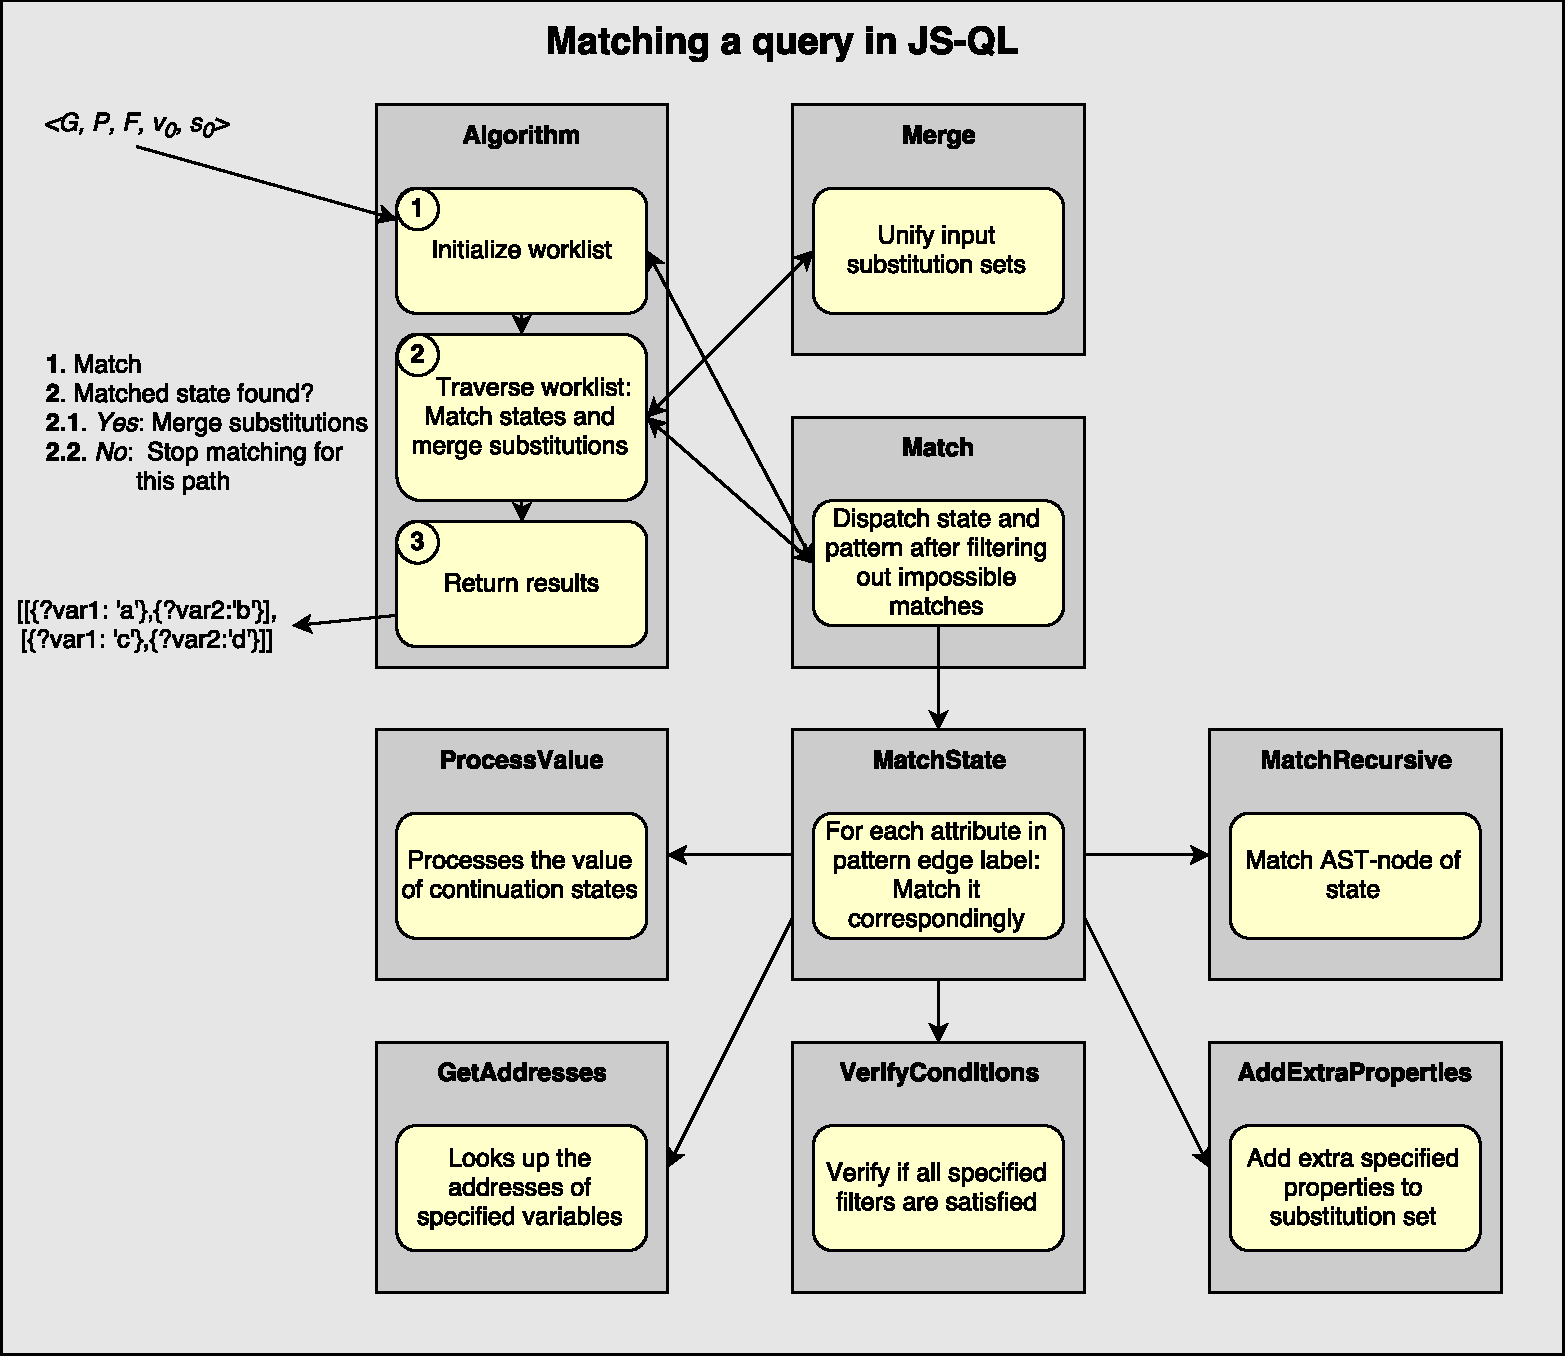
\includegraphics[width=1\textwidth]{images/matchingEngine} 
      \caption{Stages of matching a query}
    \label{fig:matchingEngine}
\end{figure}

\subsection{Inputs and output}
\label{subsec:inputOutput}
The inputs for both the existential query algorithm as the universal query algorithm are identical. In order to to match the state graph with a pattern, we have to provide both the graph and the pattern to the algorithm. The generated automaton for the pattern $P$ as well as the state graph $G$ are transformed to a uniform format, called \texttt{triples}. A triple in a pattern consists of two automaton states as source and target state and the edge between them, representing the part of state that needs to be matched (i.e. the nested map of state information). For the JIPDA state graph we transformed the original graph to a similar representation, as already described above. The final states $F$ of $P$ also need to be specified, so that the algorithm can determine when a match is completed and its substitutions can be added to the resultset. Finally the initial states of both the automaton ($s_0$) and the state graph ($v_0$) are also required, giving the algorithm an indication on where it should start matching. Together, this information forms the 5-tuple $<G, P, F, v_0, s_0>$.

The results of the algorithm consists vertex-theta pairs, where a vertex is a state in the abstract state graph and theta is the set of all possible substitutions for the query ending in that state. In our implementation, we call these pairs \texttt{VertexThetaPair}s, and they form the tuple $<v, \theta>$.

\subsection{Query algorithms}
\label{subsec:algorithms}

The semantics of both algorithms can be divided into two main phases. The first phase creates and initializes the worklist, while the second phase processes each element in the worklist and adds new elements to it as long as a pattern is matched. We describe both phases in this section for existential queries, and explain the differences with the algorithm for solving universal queries.


\subsubsection*{The worklist initialization phase}
 The first part consists of initializing the worklist. This worklist $W$ contains triples of the form $<v, s, \theta>$, where $v$ is a state of the state graph, $s$ a state of the automaton and $\theta_s$ the set of substitutions that have been matched up until $s$ in the pattern. The algorithm loops over each state in the state graph to locate a triple $t_G$ in $G$ having the starting state $v_0$ as its source. Next, all triples in $P$ are traversed until initial state $s_0$ is found as the source state of a triple $t_P$. When both triples are found their edge labels are \textit{matched}. If the matching succeeds, a list of all possible substitutions $\theta$ is returned and the worklist gets updated to contain the destination states of $t_G$ and $t_P$ together with a substitution from $\theta$. Producing a match from two edge labels is discussed in section \ref{subsec:matching}. If no match between $v_0$ and $s_0$ is found, the query fails and no results are returned, as a match for the initial states can not be found anywhere in the state graph.

\subsubsection*{The worklist processing phase}
In the second phase of the algorithm, worklist $W$ gets traversed. $W$ contains a state $v$ of the state graph, a state $s$ of the automaton and the partial match and substitution set $\theta$ between these two states. Each successor ($v_{succ}$ and $s_{succ}$) of both $v$ and $s$ are tried as the next match in a pattern, unless $s_{succ}$ is a state in the automaton representing a subgraph. If this is the case the pattern gets expanded, as isexplained in section \ref{subsec:subgraphs}. When a match is found, each found substitution $\theta_{succ_i}$between $v_{succ}$ and $s_{succ}$ is merged with $\theta$. If this merge succeeds, the triple $<v_{succ}, s_{succ}, \theta_{succ_i}>$ is added to $W$, only if it hasn't already been processed in an earlier matching step. This is called \textit{fixpointing}, and is applied by keeping track of the already reached triples in the reach list $R$ in order to prevent the algorithm from looping forever. The merging process is described in more detail in section \ref{subsec:merging}. 

After acquiring the next triple(s) for the worklist for a certain $v$ and $s$, the algorithm checks whether $s$ is contained in the list of final states $F$. If it does, a \texttt{vertexThetaPair} is added to the resultlist containing $v$ (the state of the graph matching the final state of the pattern) and $\theta$ (the set of all substitutions between $v_0$ and $v$). When the worklist is depleted, no more paths need to be matched, indicating that all possible results have been collected. All \texttt{VertexThetaPair}s are returned so that they can be processed in the user interface layer.

\subsubsection*{Differences with the algorithm for universal queries}
 The algorithm described in the previous section is used to solve existential queries. Universal queries use an algorithm which is very similar, except that it performs an extra check for the \textit{determinism condition} in the second phase of the algorithm. 
\begin{definition}
\textit{The \textbf{determinism condition} imposes that for each path from $v_0$ to $v$ in $G$, all paths in $P$ that match it (under any substitutions) pass through the same set of states.}
\end{definition}
 We implement this condition by setting a flag when a match is found for one path in $P$. If a match is found for another path in $P$, the determinism condition is violated and the matching engine halts execution. In this case, no results will be produced. Another condition for universal queries to produce results is that for each matching state in $G$, the corresponding state in $P$ should be a final state. This last condition is rather trivial, as queries only produce a result if they are matched up until a final state.

\subsection{Matching states with a pattern}
\label{subsec:matching}

Matching in the strict sense of the word means checking if two things are equal. In our implementation, a match occurs when a state in $P$ is \textit{subsumed} by a state of $G$. What this means is that all the information that is contained in a state in the pattern has to occur in the state of the state graph that is currently being matched, allowing the latter to contain more information than only what is specified by the pattern state. Figure \ref{fig:matchingPredicates} illustrates how a state is matched. The JS-QL predicate on the right produces a match, as it is subsumed by the JIPDA state. In contrast, the left JS-QL predicate specifies a \texttt{callee} attribute, which is not contained in the JIPDA state. This suffices to produce a mismatch, leading to a failed match for the currently matched path in the state graph.
\begin{figure}[!h]
    \centering
      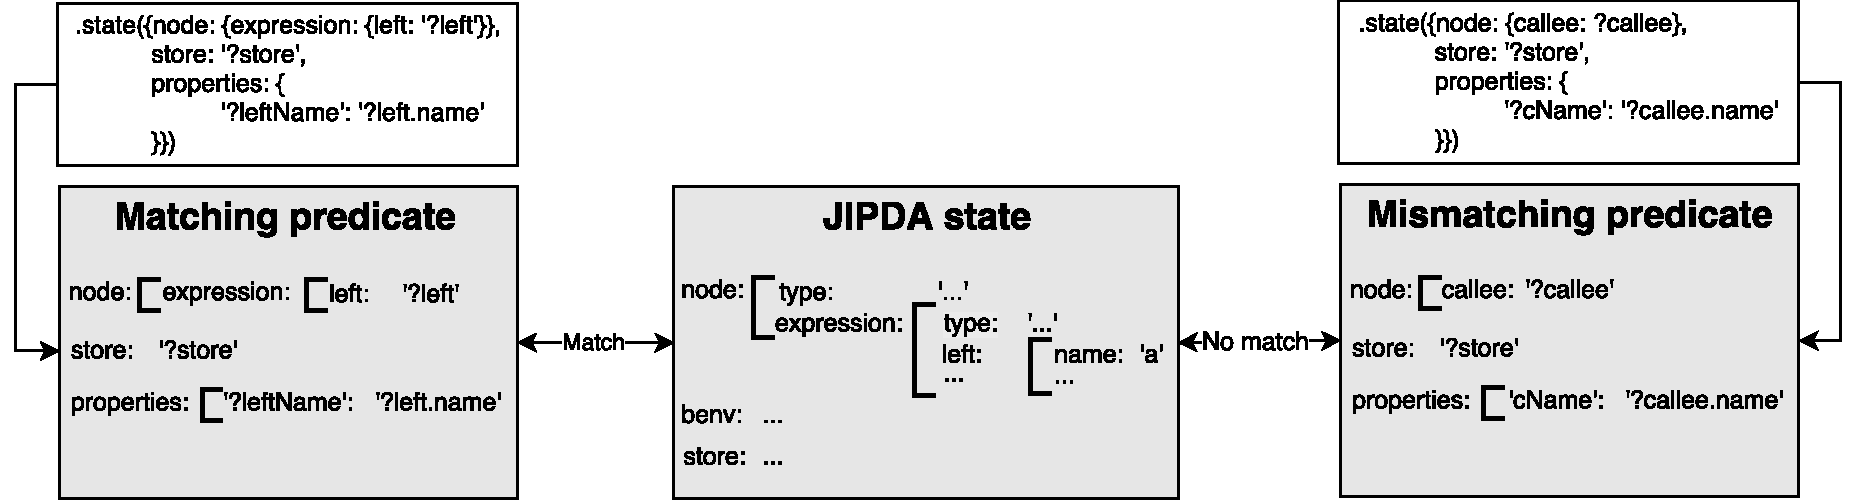
\includegraphics[width=1\textwidth]{images/matchingPredicates} 
      \caption{A matching and mismatching predicate for a JIPDA state}
    \label{fig:matchingPredicates}
\end{figure}

The JS-QL tool matches states using the \texttt{match} function. This function is an entry point to the matching process, as it only passes all matching work to the \texttt{matchState} function and waits for its results. \texttt{match} however does perform an initial check to make sure no excessive work is done: when encountering a wildcard in the pattern, no matching needs to be done as a wildcard matches any state. Negation is also handled by this function: matching a negated pattern state consists of matching the regular state (i.e. the state without negation) and returning false when a match is found and the empty substitution list otherwise. 

The remainder of this section discusses the different phases of the matching processas depicted in figure \ref{fig:matchingEngine}.



\subsubsection{matchState}
The \texttt{matchState} function is responsible for delegating the matching of keywords and combining the results of those matches. The initial substitution set $\theta$ is empty and grows larger for each keyword that is matched. Internally, the function works as follows: for each keyword specified in the JS-QL query, \texttt{matchState} matches its value (i.e. a nested map, a literal or a variable) with the corresponding attribute of the state to be matched and collect the results of this partial matching. If the partial match failed, \texttt{false} is returned, elsewise the partial match is merged with $\theta$. Each possible keyword has a different processing method (see figure \ref{fig:matchingEngine}), and we briefly discuss each of them next.

\subsubsection{matchRecursive}
The \texttt{node} attribute of a state represents its corresponding AST node. This node is matched recursively until a variable or a literal is encountered. In the case of a variable, the corresponding AST node value is bound to it. If each node-attribute of the predicate is matched, the substitution set containing all matched variables is returned. There are several cases in which the \texttt{matchRecursive} function does not produce a match:
\begin{enumerate}
\item The AST node gets matched recursively until a variable or literal is encountered. In the case of a literal being matched, a mismatch occurs when the value of the literal does not agree with the value in the AST node.
\item In the other case, matching a variable which was already bound in a previous state results in a mismatch if the value of the variable can not be unified with the newly matched value.
\item The most common reason for a mismatch is when a node-attribute specified in a JS-QL query is not present in the AST node of a JIPDA state. This 'mismatching-technique' is often used instead of explicitly specifying the \textit{type} of the node in the predicate. Figure \ref{fig:matchingPredicates} illustrates this: The predicate on the right-hand side does not match as no 'callee' attribute is present in the current JIPDA state.
\end{enumerate}

\subsubsection{addExtraProperties}

This function matches the properties attribute of a predicate. The matching process is split in two, using one function for each way in which properties can be defined: One function handles properties that access attributes of already bound variables. The other function handles properties specified by \texttt{prop}. Both functions first resolve all needed variables, and fail to match if one or more variables cannot be resolved (i.e. are not contained in the current substitution set). After resolving all used variables, the new variables defined by the properties are evaluated and added to the substitution set to be returned. \texttt{addExtraProperties} may produce no results if any of the same reasons discussed for \texttt{matchRecursive} occur.

\subsubsection{verifyConditions}

JS-QL allows to express filters, and \texttt{verifyConditions} is the function that evaluates these filters. Its internal working is similar to the matching of properties. After resolving the needed variables, the specified filter function is applied to its arguments. When the condition for a filter holds, the next filter is checked. In the case that a condition for a filter does not hold, the matching process is aborted. If all filters return \texttt{true}, the matching process can continue as the matched state meets all requirements that the filter imposes.

\subsubsection{getAddresses}
%Zoekt alle addressen op van een bepaalde naam. gebruikt hiervoor benv en store.
The \texttt{getAddresses} function looks up the addresses for the variable specified in the lookup map. Because of the precision loss due to abstract interpretation, variables can have multiple addresses. For each name in the map, a literal or a variable to be resolved, the addresses are looked up using the binding environment and the store. When no address is found for the specified name (meaning that the variable does not exist at that point in the program), the matching process fails.

\subsubsection{processValue}
Continuation states have a 'value' attribute. This attribute contains the addresses or values for an expression or statement that has been evaluated. The \texttt{processValue} function duplicates the existing substitution set and adds one address/value to each of the duplicated substitution set. The resulting substitution sets each contain one possible value or address.



\subsection{Merging substitution results}
\label{subsec:merging}

Merging happens when the substitution set of previously matched state in the pattern has to be combined with the newly acquired substitution set for the currently matched state. When these substitution sets can be combined, a valid next step in the state graph is found with the newly created substitution set $\theta_{res}$. Else, the algorithm halts for the current path in the state graph, as the substitution sets can not be merged. Merging in our tool is fairly straightforward. 

A merge between two substitution sets $\theta_i$ and $\theta_j$ only succeeds if no substitution of $\theta_i$ is contradicted by a substitution in $\theta_j$, and vice versa. When one substitution set contains a substitution that is not contained in the other, the resulting substitution set will also contain that substitution. Two contradicting substitutions result in a mismatch, making the algorithm halt for the currently matched path. The merging process is illustrated in example \ref{ex:Merging}.
\begin{exmp}
\label{ex:Merging}
Table \ref{tab:merging} shows the possible outcome $\theta_{res}$ of merging two substitution sets $\theta_{i}$ and $\theta_{j}$.

\begin{table}[!h]
\centering
  \begin{tabular}{| c | c | c | c |}
  \hline
   & $\theta_i$ & $\theta_j$ & $\theta_{res}$\\
  \hline \hline
  %\{?var1: 'a'\}, \{?var2: 'b'\} & \{?var3: 'a'\} & \{?var1: 'a'\}, \{?var2: 'b'\}, \{?var3: 'a'\} \\
  \multirow{3}{*}{1} & ?var1: x & ?var3: x & ?var1: x\\
    & ?var2: y &  & ?var2: y\\
    & & & ?var3: x\\
  \hline
  2 & ?var1: x & ?var1: y & false\\
  \hline
   \multirow{2}{*}{3} & ?var1: x & ?var1: x & ?var1: x\\
  & & ?var2: y & ?var2: y \\
  \hline

  \end{tabular}
  
  \caption{Examples of merging two substitution sets}
  \label{tab:merging}
\end{table}

 The first entry in the table succesfully merges the two sets because they are contain disjunct information. No overlaps in variables occur, so the resulting set is the union of both sets. A mismatch is encountered in the second entry. The substitution value for \texttt{?var1} in $\theta_i$ differs from that in $\theta_j$, resulting in a failed merge. The last entry again poses no problem to merge as \texttt{?var1} contains the same value in both sets and \texttt{?var2} is only contained in the second set.

\end{exmp}
\subsection{Processing subgraphs}
\label{subsec:subgraphs}

Recursive query calls in pattern $P$ are represented by a single state of type 'subgraph'. When encountered in a query solver algorithm, this state has to be expanded in such a way that the pattern gets modified to contain \textit{one} additional recursive step. The query solver algorithms used by JS-QL match a state of graph $G$ with a state of $P$, and halts the matching process for that path when no match is found. This has as a side effect that we indeed do not have to try and exhaustively expand each subgraph state, because the algorithm might never reach the expanded states. Another consideration is that if we were to expand the subgraph state multiple times, the algorithm might get trapped in an infinite loop as it does not know when to stop exploring recursive steps. 

Figure \ref{fig:subgraphExpansion} shows what happens when a recursive state of the \texttt{taintedBy} policy is encountered by a solver algorithm. We see that the subgraph in the original policy gets replaced by the entire pattern of that policy in the first recursive step.

\begin{figure}[!h]
    \centering
      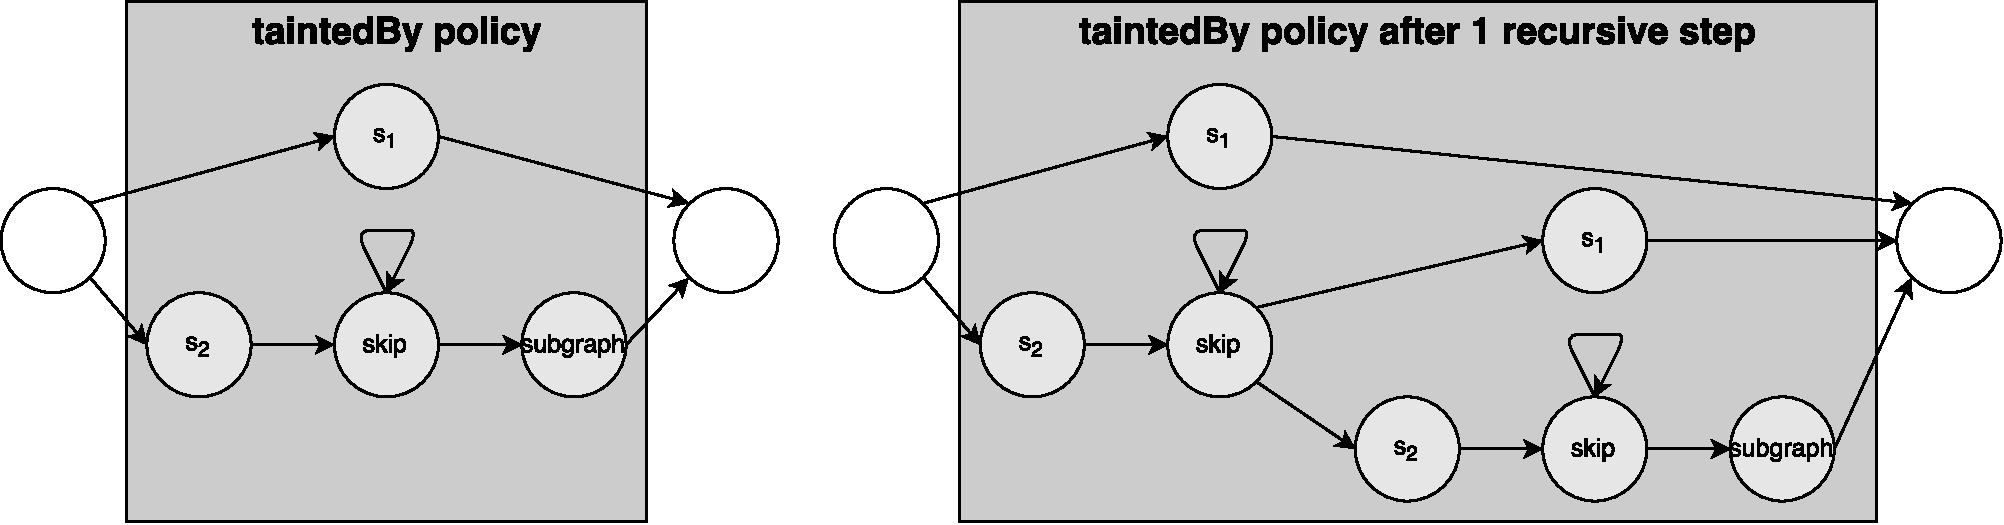
\includegraphics[width=1\textwidth]{images/subgraphExpansion} 
      \caption{Before and after expanding a subgraph for one recursive step}
    \label{fig:subgraphExpansion}
\end{figure}

Expansion of a subgraph state happens by applying the \texttt{expandFunction} (section \ref{sec:queryLanguageImpl}), which is a predicate or policy returning a piece of a pattern $P_{subgraph}$, and replacing the subgraph state in $P$ by the obtained pattern $P_{subgraph}$. The same subgraph may be expanded for different paths in the state graph, resulting in costly computations for each of those paths. We remedy this by caching each expanded subgraph. Each subgraph state (with its unique identifier) is mapped to its expanded subgraph pattern. When in the next iteration of the algorithm a subgraph state is encountered, its corresponding subgraph pattern is first looked up in the cache. Only when there is no corresponding subgraph available, the subgraph is calculated and added to the cache.


\section{Conclusion}

In this chapter we discussed the implementation of the JS-QL tool. As the code of our tool is logically subdivided in several functionality layers, we describe the architecture of the tool and discuss each component in it. We provide an overview of the user interface, and explain how it can be used and interpreted. Our tool uses the JS-QL query language to express queries, and we describe several implementation techniques used to build JS-QL. Finally, we also discuss the workings of the matching engine, which is the core of the tool. We explain how queries are matched and results are merged, and describe how results are accumulated.



 
\chapter{Evaluation}
\label{ch:Evaluation}
In this chapter we validate and evaluate the expressiveness of the JS-QL query language by expressing some existing security policies, described in other related work, in our own query language. We will then compare these policies in terms of expressiveness and flexibility. %TODO: Vergelijken op welke manier
The concept and approach for creating a new, domain-specific language for security policies is explained in chapter \ref{ch:QueryLanguage}. Chapter \ref{ch:QueryEngine} discusses the underlying query engine and how it works together with the query language to process the application-specific policies. In chapter \ref{ch:Implementation} we explain how our approach was instantiated.

We start this chapter by expressing 9 security policies distilled from 3 papers in sections \ref{sec:ValidationPidginQL}, \ref{sec:ValidationGK} and \ref{sec:ValidationConscript} respectively. Every JS-QL policy will be evaluated by comparing how well it matches the policy expressed in the original paper. Finally, in section \ref{sec:ValidationEvaluation}, we evaluate the query framework by specifying its advantages, disadvantages and limitations. We will also briefly compare the query languages presented in this chapter in terms of expressiveness, verbosity and conciseness (\textit{LOC}).
%TODO: wat gaan we nog comparen?
%TODO: JAVASCRIPT SOURCE CODE ADDEN
\section{the GateKeeper language}
\label{sec:ValidationGK}

In this chapter we attempt to express 3 policies originally presented in \cite{GateKeeper}.

\subsection{Writes to prototype objects}

Many websites use bookmarklets to store user information to automate the login process, for example \cite{PrototypePoisoning}. This is a common strategy used to reduce the amount of information the user has enter every time he visits the website. An attacker website however, can alter the JavaScript environment in such a way that he can steal all of this information from the user. Imagine a simple login function, which checks the current location of the webpage to verify that it is on the correct webpage. The current location can be compromised by overwriting the \texttt{toString} function of the \texttt{String} object, as depicted in \ref{lst:PrototypePoisoning}. This function can be configured to always return a "good" location. In this way, the login function will be called in the environment of a malicious website, possibly leaking sensitive information.

\begin{lstlisting}[label={lst:PrototypePoisoning},language=JavaScript,caption=Prototype poisoning example,mathescape=true]  % float=t?

String.prototype.toString = function(){
    //Always return "spoofed" url
    return "www.goodwebsite.com";
}

var login = function(){
  if(document.location.toString() === "www.goodwebsite.com"){
    //leak information on untrusted website
  }
}
\end{lstlisting}

%gatekeeper doet het zo
Gatekeeper expresses policies by defining a set of rules in datalog. In order to detect writes to prototypes of frozen objects, they define the \texttt{FrozenViolation(v)} predicade, as shown in listing \ref{lst:Policy1GK}. This predicate first looks for all stores of field \texttt{v}. This field points to location \texttt{h2}, which represents the points-to address for variables. Only writes to builtin objects are infringements of the policy, which implies that \texttt{h2} has to point to a field of of one of these objects. This is expressed as follows: In \texttt{BuiltInObjects(h)}, \texttt{h} points to the heap location of a builtin object. The \texttt{Reaches(h1,h2)} predicate makes sure that the field that was stored reaches the builtin object directly or indirectly, by recursively checking if one of the properties of the builtin object has a field pointing to the stored field.

\begin{lstlisting}[label={lst:Policy1GK},language=Prolog,caption=Policy 1 in GateKeeper,mathescape=true]  % float=t?

Reaches(h1,h2) :- HeapPtsTo(h1,_,h2).
Reaches(h1,h2) :- HeapPtsTo(h1,_,h3),
                  Reaches(h3,h2).

FrozenViolation(v) :- Store(v,_,_),
                      PtsTo(v,h2),
                      BuiltInObject(h1),
                      Reaches(h1,h2).

% Specify all built in objects
BuiltInObject(h) :- GlobalSym("String", h).
BuiltInObject(h) :- GlobalSym("Array", h).
% ...

GlobalSym(m,h) :- PtsTo("global", g),
                  HeapPtsTo(g,m,h).

\end{lstlisting}

%ik doe het zo (geef voorbeeld voor ééntje, zeggen dat we een compound query hebben gemaakt voor om te bundelen)
Writing this policy in JS-QL is easy. To ease the work for the programmer, we augmented the Jipda-nodes corresponding with \texttt{MemberExpression}s two extra fields: \texttt{mainObjectName} and \texttt{properties}, representing the root object and the property-chain array that was accessed respectively. An example: for \texttt{o.x.y.z}, \texttt{o} would be the \texttt{mainObjectName}, and \texttt{[x,y,z]} would be the array \texttt{properties} which represents the properties that were chained. Listing \ref{lst:Policy1JSQL} depicts the JS-QL query to efficiently express this policy. Note that the filter on lines 10-12 can be omitted. This filter simply indicates that we only want to detect writes to the \texttt{prototype} property of the \texttt{String} object. When this is omitted, we will detect all writes to this object.

\begin{lstlisting}[label={lst:Policy1JSQL},language=JavaScript,caption=Policy 1 in JS-QL,mathescape=true]  % float=t?

G.skipZeroOrMore()
.state({
  node:{
    expression:{
      left:{
        properties: '?props',
        mainObjectName: 'String'
      }
    }
  },
  filters:[
    cond('contains', '?props', 'prototype')
  ]
})

\end{lstlisting}

This example JS-QL policy only detects writes to the \texttt{String} object. We wrote a compound policy \texttt{writeToBuiltinObjectPrototype} to detect writes to all builtin objects' prototype property. The code for this policy can be found in listing \ref{lst:WriteToBuiltinObjectPrototype} in the appendix. This policy is just the disjunction of states similar to the state in listing \ref{lst:Policy1JSQL}, with the only difference in the \texttt{mainObjectName} property, which corresponds to a different builtin object name.
%TODO: bespreken

\subsection{Global namespace pollution}

Working in a JavaScript environment often involves the inclusion of multiple (third-party) scripts. These scripts offer instant access to functionality which would be tiresome to implement for every project yourself. Some of these scripts are written by other parties, so one can't be sure that they follow the same coding guidelines as he does. Inexperienced programmers might not be aware of the JavaScript namespacing patterns \cite{JSNamespacing}. This leaves an open window for a phenomenon called "global namespace pollution". Defining variables in the global scope in JavaScript can lead to unanticipated behaviour of the program when another script defines a global variable with the same name.

Preventing stores to the global object (i.e. in the global scope) can be enforced through a simple two-lined GateKeeper policy. GateKeeper handles the global object explicitly by defining a variable \texttt{global}. Global variables can then be simulated as fields of this object. Note that JIPDA does this in a similar way. A policy to detect global stores can then be defined as in \ref{lst:Policy3GK}: The global object variable is located on address \texttt{g}. Every field store \texttt{h} that points to a field of \texttt{g} will then be detected by the \texttt{GLobalStore}.

\begin{lstlisting}[label={lst:Policy3GK},language=Prolog,caption=Policy 3 in GateKeeper,mathescape=true]  % float=t?

GlobalStore(h) :- PtsTo("global",g),
                  HeapPtsTo(g,_,h).
\end{lstlisting}


\subsection{Script inclusions}

A well known exploit in JavaScript environments is \textit{heap spraying}. This is an attacking technique that can eventually even compromise a user's system. In short, it arranges the layout of the heap by allocating a vast amount of carefully-chosen strings, installing a certain sequence of bytes at a predetermined location in the memory of a target. When this is achieved, the exploit is triggered. This trigger depends on the user's operating system and browser. Such an agressive attack can be instantiated on the victim's computer by simply including a malicious script. This could be a reason to write a policy which detects all script inclusions. Regular script inclusions through \texttt{<script></script>} tags can be detected by hand. Javascript however also allows programmers to write arbitrary HTML code by using the \texttt{document.write} and \texttt{document.writeln} functions. Listing \ref{lst:ScriptInclusion} gives an example of malicious script inclusions.

\begin{lstlisting}[label={lst:Policy2GK},language=JavaScript,caption=Script inclusion example,mathescape=true]  % float=t?

var evilScript;
var scripts = ["<script>bad1</script>","<script>bad2</script>"];

for(var i = 0; i < scripts.length; i++){
  evilScript = scripts[i];
  document.write(evilScript); //violation
}

var o = {};
o.f = document.writeln;
o.f("<script>bad3</script>"); //Violation
\end{lstlisting}

This policy can be written with only a few lines of datalog in GateKeeper. What needs to be detected are the calls to \texttt{document.write/document.writeln}, even when they are aliased. This is important to note because scripts used for attacks are often obfuscated. The policy in listing \ref{lst:Policy2GK} does just that. \texttt{DocumentWrite(i)} first looks for the address \texttt{d} on the heap which points to the global \texttt{document} object. Next, the location of the property \texttt{write/writeln} of that object is reified in variable \texttt{m}. This is also an address on the heap. The last step is to find all call sites \texttt{i} that point to that same address on the heap. 

\begin{lstlisting}[label={lst:Policy2GK},language=Prolog,caption=Policy 2 in GateKeeper,mathescape=true]  % float=t?

DocumentWrite(i) :- GlobalSym("document",d),
                    HeapPtsTo(d,"write",m),
                    Calls(i,m).

DocumentWrite(i) :- GlobalSym("document",d),
                    HeapPtsTo(d,"writeln",m),
                    Calls(i,m).
\end{lstlisting}

JS-QL also proves to be suitable to express such a policy in listing \ref{lst:Policy2JSQL}. The approach we take first skips zero or more states in the JIPDA graph. We specify that we then want to find a function call with the name of the function bound to metavariable \texttt{?name}. In order to know to which address the called function points in the store, we look it up and bind the address to \texttt{?addr} in the lookup-clause of the \texttt{fCall} predicate. Finally we also match the address of \texttt{document.write/document.writeln} to the same \texttt{?addr} metavariable, filtering out all function calls that do not point to this address.

The analysis that we use is context-sensitive and Javascript is lexically scoped. This implies that we need to explicitly specify that we are looking for the address of the \textit{global} \texttt{document.write/document.writeln} object. If we didn't do this and the user has defined an object with the name "document" and a property "write" or "writeln" inside the scope of the current node in the graph, we would get the address of that object instead of the global object. That is why JS-QL provides a \texttt{\_global} keyword which indicates that we need to search for the address in the global namespace. 

\begin{lstlisting}[label={lst:Policy2JSQL},language=JavaScript,caption=Policy 2 in JS-QL,mathescape=true]  % float=t?

G.skipZeroOrMore()
.lBrace()
.fCall({
  name: '?name',
  lookup:{
    '?name'   : '?addr',
    '$\_$global.document.write': '?addr',
    }
})
.or()
.fCall({
  name: '?name',
  lookup:{
    '?name'   : '?addr',
    '$\_$global.document.writeln': '?addr',
    }
})
.rBrace()
\end{lstlisting}

%GK is flow insensitive, mijn vb gaat meer vinden

\subsection{Conclusion}

\section{The PidginQL language}
\label{sec:ValidationPidginQL}

In this chapter we attempt to express 3 policies originally presented in \cite{PidginQLTechReport}.
%TODO uitleggen hoe zij hun graph voorstellen (verwijzen naar RW).

\subsection{Only CMS administrators can send a message to all CMS users}
%Context uitleg
Imagine a situation where not only administrators can send broadcast messages. A regular user with bad intentions could easily take advantage of this situation to cause harm to the system. A CMS application for instance with a decent size of users could be exploited by sending a message to all users, asking them to reply with their password. When the attacker provides a reason to the victims convincing them to send their password, he could possibly compromise the contents of the victim's account. An example of such a reason could be that the 'administrator' needs to have the password of a user account in order to update the software of that user to the latest version. This behaviour is undesirable, thus we need a policy which prevents regular users from sending such messages.

The policy listed in \cite{PidginQLTechReport} that addresses this issue can be found in listing \ref{lst:Policy4PidginQL}. First, all nodes that are entries of the \texttt{addNotice} method are searched for and stored in a variable. \texttt{addNotice} is the method that sends messages to all users, and has the same behaviour as the broadcast method in the explanation above. Next, all points in the PDG are found that match a return node of the \texttt{isCMSAdmin} method with a return value which is truthy. In order to know if there exists some path in the graph where \texttt{addNotice} is called when the return value of \texttt{isCMSAdmin} is false, all paths between the nodes in \texttt{addNotice} and \texttt{isAdmin} are removed from the graph for all paths where \texttt{isAdmin} is true. Finally, the intersection of the nodes in this 'unsanitized' graph and the nodes in the \texttt{sensitiveOps} argument is taken. When this intersection is not empty, we can assume that there is a violation of the policy in the remainder of the graph. This last part is exactly what the \texttt{accessControlled} method does.

%AccessControlled = let accessControlled(G, checks, sensitiveOps) = G.removeControlDeps(checks) ∩ sensitiveOps is empty
\begin{lstlisting}[label={lst:Policy4PidginQL},language=JavaScript,caption=Policy 4 in PidginQL,mathescape=true]  % float=t?

let accessControlled(G, checks, sensitiveOps) = 
    G.removeControlDeps(checks) $\cap$ sensitiveOps is empty

let addNotice = pgm.entriesOf("addNotice") in
let isAdmin   = pgm.returnsOf("isCMSAdmin") in 
                pgm.accessControlled(isAdmin, addNotice)
\end{lstlisting}

When attempting to write a similar query in JS-QL, we need to define the problem in terms of control flow: "There must be no path between the returns of the \texttt{isCMSAdmin}, when the return value is false, and a call of the \texttt{addNotice} method." We must note that with abstract interpretation, it is not trivial to specify whether a value is truthy or falsy. When looking at a conditional (like an \texttt{if-statement}), we can determine whether the true- of false-branch has been taken by comparing the first node of the branches with the alternate/consequent of the conditional. However, for values with the value of \textit{\{Bool\}}, we cannot decide on which branch is the true-branch and which one is the false-branch. We can solve this in two ways: We can assume that the condition in the conditional is a direct call to \texttt{isCMSAdmin}, which enables us to find the false-branch. From there on we can search for all calls to \texttt{addNotice} to find violations. The JS-QL policy for this case is defined in listing \ref{lst:Policy4JSQL}. We skip all states untill we reach the beginning of a false branch of a conditional. We bind the condition \textit{test} to the metavariable \textit{?cond}, the context \textit{kont} to \textit{?kont} and the stack \textit{lkont} to \textit{?lkont}. We further restrict condition \textit{?cond} to contain the 'callee' property, of which we take the name and match it to the 'isCMSAdmin' literal. Next, we skip some states until we find a call to the \texttt{addNotice} method. Since we only want to detect these calls within the false-branch, we end the policy with an \texttt{endIf} predicate with matching stack and context metavariables.

Another option is to find all calls to the \texttt{addNotice} method that follow a return of \texttt{isCMSAdmin}. Since we only know that the return value of \texttt{isCMSAdmin} returns a value of \textit{\{Bool\}}, we are unable to rule out any of the branching options. This will result in false-positives. Listing \ref{lst:Policy4JSQL} gives an implementation of the policy. We again match the stack and context to metavariables \textit{?lkont} and \textit{?kont}, but this time to indicate the start of a function application. Next we specify that we want to find all return statements within that function application. This is done by indicating that these return statements must follow a node which is not the end of the function application, parametrized with the same metavariables for stack and context. Finally, some states can be skipped before finding a function call to \texttt{addNotice}.

\begin{lstlisting}[label={lst:Policy4JSQL},language=JavaScript,caption=Policy 4 in JS-QL]  % float=t?

//First solution
G.skipZeroOrMore()
.beginIfFalse({test: '?cond', kont: '?kont', lkont:'?lkont', 
               properties:{
                 'isCMSAdmin' : '?cond.callee.name'
               }})
.skipZeroOrMore()
.fCall({name:'addNotice'})
.skipZeroOrMore()
.endIf({kont: '?kont', lkont:'?lkont'})

//Second solution
G.skipZeroOrMore()
.beginApply({name:'isCMSAdmin',kont:'?kont',lkont:'?lkont'})
.not()
    .endApply({ kont:'?kont',lkont:'?lkont'})
    .star()
.returnStatement()
.skipZeroOrMore()
.fCall({name:'addNotice'})

\end{lstlisting}

%Vergelijken
%Ook al vinden we bij eentje false positives, de andere matcht in principe alle calls naar addNotice als er geen isAdmin aangeroepen wordt. (Bij mij is het enkel indien gewenst [surrounden door braces en star toevoegen])
%Bij de andere is de restriction eerder JIPDA-related (statische analyse), want het framework en de taal laten wel toe om te filteren op value bijvoorbeeld
%Zij zeggen enkel of de set leeg is of niet, wij geven resultaten
%Kunnen zij velden checken?

\subsection{A database is opened only after the master password
is checked or when creating a new database}
%TODO

\begin{lstlisting}[label={lst:Policy5PidginQL},language=JavaScript,caption=Policy 5 in PidginQL,mathescape=true]  % float=t?

TODO
\end{lstlisting}

\subsection{Public outputs do not depend on a users's password, unless it has been cryptographically hashed}
%TODO

\begin{lstlisting}[label={lst:Policy6PidginQL},language=JavaScript,caption=Policy 6 in PidginQL,mathescape=true]  % float=t?

let passwords = pgm.returnsOf("getPassword") in 
let outputs   = pgm.formalsOf("writeToStorage") $\cup$
                pgm.formalsOf("print") in
let hashFormals = pgm.formalsOf("computeHash") in
pgm.declassifies(hashFormals, passwords, outputs)
\end{lstlisting}

\subsection{conclusion}

\section{The Conscript language}
\label{sec:ValidationConscript}

\subsection{No string arguments to setInterval, setTimeout}

\begin{lstlisting}[label={lst:Policy7Conscript},language=JavaScript,caption=Policy 7 in ConScript,mathescape=true]  % float=t?

let onlyFnc : K x U x U -> K =
function (setWhen : K, fn : U, time : U) {
    if ((typeof fn) != "function") {
        curse();
        throw "The time API requires functions as inputs.";
    } else {
        return setWhen(fn, time);
    }
};
around(setInterval, onlyFnc); 
around(setTimeout, onlyFnc);
\end{lstlisting}

\subsection{HTTP-cookies only}

\begin{lstlisting}[label={lst:Policy8Conscript},language=JavaScript,caption=Policy 8 in ConScript,mathescape=true]  % float=t?

let httpOnly:K->K=function(_:K){ 
    curse(); 
    throw "HTTP-only cookies"; 
};
around(getField(document, "cookie"), httpOnly); 
around(setField(document, "cookie"), httpOnly);
\end{lstlisting}

\subsection{Prevent resource abuse}

\begin{lstlisting}[label={lst:Policy9Conscript},language=JavaScript,caption=Policy 9 in ConScript,mathescape=true]  % float=t?

let err : K -> K = function () { 
    curse(); 
    throw 'err'; 
}); 
around(prompt, err); 
around(alert, err);
\end{lstlisting}

\section{Evaluation}
\label{sec:ValidationEvaluation}
%Nadeel bvb eerste policy van PidginQL: we kunnen niet naar concrete waarden kijken , bvb user.isAdmin zal {bool zijn}, maar weet niet of dit true of false is

\begin{center}
    \begin{tabular}{ | l || l | l | l |}
    \hline
    Language & Prop1 & Prop2 & Prop3 \\ \hline
    JS-QL &  &  & \\ \hline
    GateKeeper &  &  & \\ \hline
    PidginQL &  &  & \\ \hline
    Conscript &  &  & \\ \hline
    \end{tabular}
\end{center}

 
\chapter{Conclusion and future work}
\label{ch:Conclusion}
%\section{Summary}
In this dissertation proposed a query-based technique for detecting security vulnerabilities in JavaScript programs. 
Unlike most existing techniques, ours can be configured to detect vulnerabilities that are specific to a single application. To this extend we investigate JS-QL, an expressive specification language that enables users to write succinct and application-specific queries instead of using pre-encoded rules. Our language matches queries against the output graph of a statically analyzed program. More specifically, we use abstract interpretation as a static analysis technique to generate an abstract state graph representing a program.

%JS-QL enables users to write succinct and application-oriented queries, instead of limiting them to use pre-encoded patterns and analyses of a specific tool. This type of program analysis is important because the use of JavaScript as a language for all kinds of applications is increasing. This has as consequence that malicious users get more creative and passionate about finding security vulnerabilities in these applications and that more program vulnerabilities are discovered and exploited. 

The JS-QL tool combines abstract interpretation with JS-QL, a novel program specification language that enables developers to test their applications against these vulnerabilities. JS-QL is a domain-specific language embedded in JavaScript and is based on the concept of regular path expressions. These expressions are similar to traditional regular expressions, except that they can be applied to find certain paths in a graph instead of finding patterns in a string. Other approaches are described in related work (Sections \ref{sec:genericVulnerabilities} and \ref{sec:applicationSpecificVulnerabilities}), but none of them use abstract interpretation to model the flow of programs.

 %JS-QL queries provide sufficient expressiveness to detect security vulnerabilities in programs in a way that is especially readable. 
 We evaluate our specification language by expressing multiple security vulnerabilities and comparing the resulting specifications to corresponding ones of existing work.
 The results of the evaluation indicate that the static analysis of our technique is sufficiently powerful while its specification language is sufficiently expressive for application-specific vulnerabilities commonly found in related work. We also provide a tool together with a minimalistic user interface serving as a means to apply JS-QL queries to JavaScript programs, reporting all results of a query in both a visual (graph) representation and a textual representation. 

 We conclude from our experiments that our language is apt for specifying several types of security vulnerabilities. These specifications are often more readable, concise and equally expressive compared to their notation in other languages. 

%Nu bespreken we limitations
\section{Technical limitations of the approach}

This section discusses the limitations of the tool. We seek to find appropriate solutions for all of the following limitations of the tool in future work.

\subsection*{Negation}

As discussed in section \ref{sec:Syntax}, negation is supported by the JS-QL language. The current implementation however is limited to the negation of only one state, which sometimes does not suffice. Consider a situation in which a state in the state graph must be matched with all but two specific states \texttt{stateA} and \texttt{stateB}. To match this state, it would be convenient to be able to express a pattern in JS-QL like \\\texttt{not().lBrace().stateA().or.stateB().rBrace()}\\indicating that neither states must be matched for a certain state in the state graph. This functionality is not available in the current iplementation of JS-QL. 

One could also argue that it would be useful to specify the negation of a single value in a state. In this way, one could for example express that they wish to find all variable declarations, except for variables with name 'a'. The relevant code in the state map would then be: \texttt{\{name: '$\neg$a'\}}. Although this notation might be useful, JS-QL already supports queries with the same semantic value, by using a simple filter indicating that the name can not be equal to 'a'.

\subsection*{Performance}

Our current implementation has some computational overhead as each state edge label $el$ and pattern label $tl$ can be matched multiple times in the algorithm. Each match is a computationally heavy operation, which means that we should try to avoid matching $el$ and $tl$ more than once. This could be done by memoizing the substitutions between all already matched pairs of state and pattern, decreasing the computational overhead drastically. This approach would make the tool scale in two ways: (i) The JavaScript programs to be queried can be of larger size because (ii) the algorithms used would saturize more quickly, resulting in faster query results. Currently, all programs and queries tested run within reasonable time ($<$ 3 seconds), but we expect that for larger programs and queries the run-time of the tool would increase significantly. However, the goal of this thesis was to investigate whether regular path queries can be used to effectively specify and detect security vulnerabilities, rather than to build a performant tool to process these queries.

\section{Future research}

This section discusses the subjects of interest for future research. We believe that research in these areas can be fruitful for both the JS-QL language as well as other approaches for detecting security vulnerabilities.

\subsection*{A library of security vulnerabilities}
Our experiments show how security vulnerabilities originating from related work can be expressed in JS-QL. Gathering more security vulnerabilities to express will grant us insight on several recurring patterns used to exploit application flaws. The exploration of vulnerabilities and vulnerability types can lead to the creation of more specific and precise constructs in JS-QL that are optimal for expressing these security vulnerabilities.

\subsection*{Querying other program representations}
JS-QL was designed to work on the JIPDA state graph. We would like to investigate how much work is needed to port JS-QL to support other graphs. Hypothetically, only the matching process has to be altered, as other graphs will contain information that is structured differently. %This investigation could even be extended if we consider other program representations, such as Datalog. We suspect that this would involve much more work. We can keep the JS-QL language as the language to express policies, but we would have to develop a whole new mechanism (i.e. a compiler) to translate JS-QL queries to Datalog-queries.

\subsection*{Combining results}

A gread addition to JS-QL would be the ability to combine results of queries. This would make it easier for the user to detect multiple vulnerabilities at the same time, and it would make the language more expressive. Combining results could be implemented as a simple conjunction operation, but could also be defined as a more complex operation between results, such as an exclusive disjunction for example. The usefulness of the latter has already been proven in our experiments (\ref{subsec:CMSAdmin}).

\section{Concluding remarks}
%TODO
We started this dissertation by investigating which approach would fit best for detecting security vulnerabilities in JavaScript programs. We presented the JS-QL tool, a tool for expressing and checking security vulnerabilities against an abstract state graph. The tool uses the novel JS-QL language, which is based on regular path expressions. 
%This type of language for expressing queries is useful for specifying security policies (as shown in chapter \ref{ch:Evaluation}). 

We believe that our tool represents a step in the right direction for allowing users to preventively detect security vulnerabilities in their JavaScript applications. By shifting the emphasis from general policies to application-specific policies, security vulnerabilities can be expressed in a more fine-grained way when using the JS-QL tool. 


\begin{appendices}
\chapter{JS-QL policies and predicates}

\begin{lstlisting}[label={lst:OpenClosedFile},language=JavaScript,caption=A query for detecting accesses to closed files,mathescape=true]  % float=t?

G.skipZeroOrMore()
.state({node:{
          expression:{
            callee : {name : 'close'},
            arguments: '?args'
        }},
        properties:{
          '?arg' : prop('memberOf','?args'),
          '?argName': '?arg.name'
        },
        lookup:{
          '?argName': '?argAddr' //Match address of the file
        }
       })
.not()
.state({node:{
          expression:{
            callee : {name : 'open'},
            arguments: '?args2'
        }},
        properties:{
          '?arg2' : prop('memberOf','?args2'),
          '?argName2': '?arg2.name'
        },
        lookup:{
          '?argName2': '?argAddr'
        }
       }).star() //Zero or more states
.state({node:{
          expression:{
            callee : {name : 'access'},
            arguments: '?args3'
        }},
        properties:{
          '?arg3' : prop('memberOf','?args3'),
          '?argName3': '?arg3.name'
        },
        lookup:{
          '?argName3': '?argAddr' //Match address of the file
        }
       })
\end{lstlisting}

\begin{lstlisting}[label={lst:assignPredicate},language=JavaScript,caption=The \texttt{assign} predicate,mathescape=true]  % float=t?

JSQL.prototype.writeToBuiltinObjectPrototype = function(obj){
  var obj = obj || {};
  var states = [];
  var frozenObjects = ['Array', 'Boolean', 'Date', 'Function', 'Document', 'Math', 'Window','String'];
  var ret = this.lBrace();
  var objProps = this.getTmpIfUndefined();
  for(var i = 0; i < frozenObjects.length; i++){
    var s = {};
    this.setupStateChain(s, ['node', 'expression', 'left','properties'], objProps);
    this.setupStateChain(s, ['node', 'expression', 'left','mainObjectName'], frozenObjects[i]);
    this.setupFilter(s, 'contains', objProps, 'prototype');
    this.finalize(s, obj);
    states.push(s);
  }
  for(var j = 0; j < states.length; j++){
    if(j !== states.length - 1){
      ret = ret.state(states[j]).or()
    }
    else{
      ret = ret.state(states[j]).rBrace();
    }
  }
  return ret;
}
\end{lstlisting}

\begin{lstlisting}[label={lst:taintedBy},language=JavaScript,caption=The \texttt{taintedBy} recursive policy,mathescape=true]  % float=t?
JSQL.prototype.taintedBy = function(obj){ //x, y, rec
  obj = obj || {};
  var s1 = {};
  var s2 = {};
  var newObj = {};
  var x = this.getTmpIfUndefined(obj.x);
  var y = this.getTmpIfUndefined(obj.y);
  var flow;
  
  if(obj.rec){
    flow = this.getRecVar(obj.rec);
  }
  else{
    flow = this.getTmpIfUndefined();
  }

  newObj.x = flow;
  newObj.y = y;
  newObj.rec = obj.rec;

  this.setupStateChain(s1, ['node','expression','right','name'], x); //alias
  this.setupStateChain(s1, ['node','expression','left','name'], y); //leaked
  this.setupStateChain(s2, ['node','expression','right','name'], x); //alias
  this.setupStateChain(s2, ['node','expression','left','name'], flow); //leaked

  return this .lBrace()
        .state(s1) //assign from x to y
        .or()
        .state(s2) //assign from x to tmp
        .skipZeroOrMore()
        .rec(newObj,this.taintedBy)
        .rBrace();

}
\end{lstlisting}

\begin{lstlisting}[label={lst:WriteToBuiltinObjectPrototype},language=JavaScript,caption=The \texttt{writeToBuiltinObjectPrototype} policy,mathescape=true]  % float=t?

JSQL.prototype.writeToBuiltinObjectPrototype = function(obj){
  var obj = obj || {};
  var states = [];
  var frozenObjects = ['Array', 'Boolean', 'Date', 'Function', 'Document', 'Math', 'Window','String'];
  var ret = this.lBrace();
  var objProps = this.getTmpIfUndefined();
  for(var i = 0; i < frozenObjects.length; i++){
    var s = {};
    this.setupStateChain(s, ['node', 'expression', 'left','properties'], objProps);
    this.setupStateChain(s, ['node', 'expression', 'left','mainObjectName'], frozenObjects[i]);
    this.setupFilter(s, 'contains', objProps, 'prototype');
    this.finalize(s, obj);
    states.push(s);
  }
  for(var j = 0; j < states.length; j++){
    if(j !== states.length - 1){
      ret = ret.state(states[j]).or()
    }
    else{
      ret = ret.state(states[j]).rBrace();
    }
  }
  return ret;
}
\end{lstlisting}



\end{appendices}

\printbibliography
\end{document}